\documentclass[11pt,a4paper, twoside]{book}
\usepackage[a4paper, top=3.5cm, bottom=3.5cm,%
marginparwidth=2.7cm, marginparsep=0.3cm]{geometry}
\usepackage[utf8]{inputenc}
\usepackage{amsmath}
\usepackage{amsthm}
\usepackage{amsfonts}
\usepackage{amssymb}
\usepackage{bbm}
\usepackage{tikz}
\usepackage{bm}
\usetikzlibrary{arrows}
\usepackage{subcaption}
\usepackage{graphicx}
\usepackage{natbib}
\usepackage{multirow}
\usepackage{booktabs}
 \usepackage{hyperref}
\usepackage{afterpage}
\usepackage{fancyhdr}
%\usepackage{titlesec}
%\titleformat{\chapter}[display]
%{\normalfont\huge\bfseries}{\chaptertitlename\ \thechapter}{20pt}{\Huge}


\newtheorem{lemma}{Lemma}[chapter]
\newtheorem{proposition}{Proposition}[chapter]
\newtheorem{theorem}{Theorem}[chapter]
\newtheorem{corollary}{Corollary}[chapter]
\newtheorem{example}{Example}[chapter]
\newtheorem{remark}{Remark}[chapter]
\newtheorem{definition}{Definition}[chapter]
\newtheorem{observation}{Observation}[chapter]
\newtheorem{conjecture}{Conjecture}[chapter]


\newcommand{\indep}{\rotatebox[origin=c]{90}{$\models$}}
\newcommand{\Pp}{\operatorname{P}}
\newcommand{\Pq}{\operatorname{Q}}
\newcommand{\bx}{\mathbf{x}}
\newcommand{\bX}{\mathbf{X}}
\newcommand{\by}{\mathbf{y}}
\newcommand{\bY}{\mathbf{Y}}
\newcommand{\bchi}{\boldsymbol{\mathcal{X}}}
\newcommand{\nchi}{\mathcal{X}}
\bibliographystyle{plainnat}
\title{Theoretical studies on Bayesian network classifiers}
\author{Gherardo Varando}

\begin{document}
\pagestyle{empty}
%titlepage
\begin{center}
\begin{minipage}{0.85\linewidth}
    \centering
%University logo
    %\includegraphics[width=0.3\linewidth]{logo.pdf}
%    \rule{0.4\linewidth}{0.15\linewidth}\par
%    \vspace{3cm}
    
    \uppercase{\textbf{DEPARTAMENTO DE INTELIGENCIA ARTIFICIAL}}
    \vspace{1cm}
    
    {Escuela Técnica Superior de Ingenieros Informáticos \\
Universidad Politécnica de Madrid}

\vspace{3cm}  

{PhD THESIS}

\vspace{1cm}  
%Thesis title
    {\uppercase{\Large  \textbf{Theoretical studies on Bayesian network classifiers} \par}}
    \vspace{3cm}
%Author's name
    Author
    
    {\Large \textbf{Gherardo Varando}\par}
    \textbf{MS in Mathematics}
    \vspace{3cm}
    
    PhD supervisors
    \vspace{0.4cm}
    
    {\large \textbf{Concha Bielza}\par}
    PhD in Computer Science
    
    \vspace{0.2cm}
    
     {\large \textbf{Pedro Larrañaga}\par}
    PhD in Computer Science
    
    \vspace{3cm}
    
   
%Date
    {\Large 2018}
\end{minipage}
\end{center}
\cleardoublepage

\begin{center}
\Large
\textbf{Thesis Committee}
\end{center}


\paragraph{President:} Antonio Bahamonde Rionda
\paragraph{External Member:} Manuele Leonelli
\paragraph{Member:} Francisco Herrera Triguero
\paragraph{Member:} José Antonio Gámez Martín
\paragraph{Secretary:}  Emilio Serrano Fernández

\pagebreak[4]

%\cleardoublepage

\frontmatter
%\setcounter{page}{1}
\pagestyle{fancy}
\fancyhead[LE,RO]{}
\fancyhead[LO,RE]{}
\renewcommand{\headrulewidth}{0pt}


\section*{Acknowledgments}

First of all I want to express my gratitude to my supervisors, Concha Bielza and Pedro Larrañaga, for constantly supporting and motivating me.
Concha and Pedro directed the first step of my young academic career and I will always be thankful to them.   

Eva Riccomagno has guided me with incredible availability during and after the three months I had been working with her in the University of Genova. Her advices and suggestions have shaped deeply not only the research in this thesis but also my future career. 

My colleagues at the Computational Intelligence Group helped me in numerous ways through the last years. Without them the time spent in the university would have been surely less entertaining.
 
Finally I want to thank the financial support of the following projects and institutions:
Cajal Blue Brain (C080020-09), TIN2013-41592-P and TIN2016-79684-P projects, S2013/ICE-2845-CASI-CAM-CM project, Fundación BBVA grants to Scientific Research Teams in Big Data 2016, European Union Seventh Framework Programme (FP7/2007-2013) under grant agreement No. 604102 (Human Brain Project) and European Union’s Horizon 2020 research and innovation programme under grant agreement No. 720270 (HBP SGA1). The Associazione Italiana per l'Intelligenza Artificiale under the Incoming Mobility Grant and the Universidad Polit\'ecnica de Madrid under the Programa Propio 2017 for financing the research stay in the University of Genova. 


\cleardoublepage

\section*{Abstract}

Machine learning, as one of the fundamental tools of artificial intelligence, has acquired growing importance in the last decades. The increasing availability of large amounts of data and more computational processing power available at a low price have contributed to the spread of machine learning methods in almost all branches of technology. 
While a great part of the current research focuses on the creation of new algorithms and methods to tackle different problems, it is widely recognized that formal analysis and theoretical results are necessary to really understand the algorithms employed, their limitations and their capabilities. 
The work developed in the present thesis is focused on this last aspect of the research in machine learning. 

We study Bayesian network classifiers and in general generative classifiers based on probabilistic graphical models. Probabilistic graphical models are widely studied in the statistic literature and in this thesis we analyze them in the context of one of the most basic problem in machine learning, binary classification. 
Our main result is a description of the implications, for the induced decision functions, of the conditional independence  statements holding in the probability model. We will state results both for a wide class of Bayesian network classifiers and for undirected Markov network classifiers. 

In particular, we describe the classes of discrimination functions associated with some of the most used Bayesian network classifiers over categorical predictors variables. We obtain polynomials interpolating the induced discrimination functions, and thus representing the corresponding decision functions. Thanks to this characterization we are able to bound the number of decisions representable by Bayesian network classifiers with given structures.

We extend the binary classification results to chain multi-label classifiers, analyzing their expressive power when Bayesian network are used as base models. 
Finally, we describe an algebraic and geometric approach to study discrimination functions of generative classifiers under general Markov properties. The given approach extends the results for Bayesian network classifiers and introduces an elegant framework, based on finite differences, to study discrimination functions of generative classifiers.

   

\newpage 
\cleardoublepage

\section*{Resumen}

En las ultimas décadas, el aprendizaje automático ha adquirido importancia como una de las herramientas fundamentales en inteligencia artificial. El incremento en la disponibilidad de datos y capacidad computacional disponible a bajo coste han contribuido a extender los métodos de aprendizaje automático en casi todas las ramas de la tecnología. 
Mientras que gran parte de la investigación se centra en el desarrollo de nuevos algoritmos y métodos para tratar diferentes problemas, es ampliamente reconocido que el análisis formal y los resultados teóricos son necesarios para entender los algoritmos empleado, sus limitaciones y sus capacidades.
El trabajo desarrollado en esta tesis se centra en éste ultimo aspecto de la investigación en aprendizaje automático.

Estudiamos los clasificadores con redes Bayesianas y en general clasificadores generativos basados en modelos gráficos probabilisticos. Los modelos gráficos probabilisticos han sido y siguen siendo ampliamente estudiados en estadística y en esta tesis los analizamos en el contexto de uno de los problemas más representativos en aprendizaje automático, la clasificación binaria.
Nuestro resultado principal es la descripción, tanto para redes Bayesianas como para modelos de Markov no dirigidos, de las implicaciones de las independencias condicionadas en las funciones de decisión asociadas.

En particular, describimos las familias de funciones discriminantes asociadas con las familias de clasificadores con redes Bayesianas más utilizados.
Construimos polinomios que interpolan las funciones discriminantes inducidas, describiendo así las funciones de decisión. Gracias a la representación polinomial de las funciones discriminantes somos capaces de acotar el número de decisiones representables por clasificadores con redes Bayesianas.

Extendemos estos resultados a clasificadores en cadena para problemas multi etiqueta, analizando su capacidad expresiva asumiendo que los modelos están basados en redes Bayesianas.
Por último, describimos un método algebraico y geométrico para estudiar funciones discriminantes  de clasificadores generativos bajo propiedades de Markov generales. El método empleado extiende los resultados obtenido en el caso de las redes Bayesianas y describe un marco formal, basado en diferencias finitas, para estudiar las funciones discriminantes de clasificadores generativos.

 
\newpage
\cleardoublepage
\tableofcontents

\listoffigures

\listoftables
 
\cleardoublepage
\renewcommand{\headrulewidth}{1pt}


\mainmatter
\pagestyle{fancy}
\fancyhead[LE,RO]{\textsl{\MakeUppercase{\chaptername ~ \thechapter}}}
\fancyhead[LO,RE]{}
\fancyfoot[C]{\thepage}

\chapter{Introduction}

The most important and representative problem in machine learning is binary supervised classification, that is, the problem of building a model (classifier) from training data able to successively recognize a simple binary class.
Notorious examples of this problem include, but are not limited to spam filtering \citep{sahami1998}, medical testing for a given disease \citep{MORALES2013} and failure detection in industrial processes \citep{JUNG2018, varghese2015}.  

Bayesian network (BN) classifiers \citep{bielza2014} are probably the most popular example of generative classifiers and they have been employed successfully in various applications. 
Bayesian network classifiers present many advantages, as the ability of providing estimation for the posterior class probabilities, the interpretability of the  model and the inherent insights into the handled problem that a black-box algorithm is unable to provide. Moreover Bayesian Network can be built easily using a combination of data-driven knowledge and experts' opinions.

Bayesian network classifiers are based on a graphical modeling of the underlying probability distribution \citep{lauritzen1996, Pearl1988}. They range from the simplest naive Bayes~\citep{Minsky61stepstoward} classifier, where the predictor variables are assumed to be conditionally independent given the class variable, to the unrestricted Bayesian classifier, where a general form of Bayesian network \citep{Pearl1988} is permitted.

While the sound probabilistic setting of graphical models gives solid theoretical foundations to the use of Bayesian network classifiers, these methods, as every generative classifier, carry some degree of confusion on which are the induced \textit{decision functions}.
However, the so-called discriminative classifiers, usually entail naturally a description of the decision function employed (e.g., a linear function for logistic regression).

The first rigorous result about the induced decision functions of BN classifiers was given by \citet{Minsky61stepstoward}, showing that the decision boundary in naive Bayes classifiers with binary predictors is linear (a hyperplane in the Boolean hypercube). Since then some other results were provided but there is not in the literature a general study of discrimination functions induced by generative classifiers under conditional independences. This thesis intends to provide such a framework.

In this thesis we study  generative classifiers for binary class and categorical predictor variables. We focus on the expressive power and theoretical properties, firstly, of Bayesian network classifiers and lastly of general generative classifiers under Markov properties.
In the next section we state the assumptions, hypotheses and objectives of the present thesis. Then we shortly describe the structure of the manuscript.

\section{Hypotheses and Objectives}

We describe here the assumptions, hypotheses and objectives of the present thesis.

\subsubsection{Assumptions}

\begin{itemize}
\item We will only consider binary classification problems, and as an extension, multi-label problems (seen as multi binary-class problems). 
\item The predictor variables will be always categorical. Some ideas will be also extended to continuous variables, in this case assumed to be Gaussians.
\item We will always assume a probabilistic setting. That is, the class variable and the predictors are considered to be random variables, and we assume that a joint probability distribution exists.
\end{itemize}

\subsubsection{Hypotheses}

\begin{itemize}
\item It is possible to formally describe the family of decision functions representable by Bayesian network classifiers and in general generative classifiers with Markov assumptions.
\item Describing generative classifiers and their properties allow to understand some well-known intuitions in the machine learning community and suggest some ideas for developing new models. 
\end{itemize}

Based on the above hypotheses we formulate the following main objectives of the thesis:

\subsubsection{Objectives}

\begin{itemize}
\item Extend the known results about the expressive power of Bayesian network classifiers to general graphical structures and categorical predictor variables with more than two values.
\item Describe a framework to study the expressive power of generative classifiers.
\item Apply the results to multi-label methods, such as binary relevance and chain classifiers.
\item Formalize the implications of general Markov assumptions on the induced decision functions for generative classifiers.
\item Understand the implications on the generative vs. discriminative classifiers and suggest ideas about new methods for generative classifiers.
 
\end{itemize}



\section{Document Organization}

The present dissertation is divided into six chapters. The first one is the present introduction.

Background (Chapter \ref{chp:background}) contains the main mathematical definitions as well as some well-known results in the literature. It presents a simple introduction to graphs (Sec. \ref{sec:notbasic}), with useful notations to develop the theory of graphical models (Sec. \ref{sec:graphmodel}). Then, binary classification is presented (Sec. \ref{sec:classification}), with a focus on generative models and in particular Bayesian network classifiers (Sec. \ref{sec:bnclassifier}).

The following three chapters contain the original research developed during the thesis. For each chapter an individual introduction is given and conclusive sections summarize the results.
Chapter \ref{chp:decbound} contains the main results for  decision functions of Bayesian network classifiers. Chapter \ref{chp:multilabel} deals with extensions to multi-label problems, in particular chain classifiers with Bayesian networks. Chapter \ref{chp:genclas} formulates some results for generative classifiers under the undirected Markov property.


Finally, Conclusions (Chapter \ref{chp:conclusions}) summarizes the contributions of this dissertation and suggests some ideas for future research. Moreover the published contributions derived from this work are listed in connection with the corresponding chapters.


\chapter{Background}
\label{chp:background}

In this chapter we state some basic definitions and some background results about probabilistic graphical models. We also define formally binary classification problems and what we intend with generative classifiers. Moreover we give a brief introduction to Bayesian network classifiers and we review the previous approaches to the study of their expressive power.

\section{Notations and Basics}
\label{sec:notbasic}

We use bold letters, $\bx, \bX$ or $\mathbf{k}$, to represent elements of a product space, and letters with a subscript to represent the respective components. For example $x_2$ indicates the second component of $\bx$.

We denote random variables with capital letters as $X,Y,Z,X_1,X_2, X_i,X_n$. With bold capital letters we denote vectors of such random variables, and with subscripts we indicate the components of the vector as follow:
$$ \bX = (X_1, X_2, \ldots , X_n).$$

With $x,x_1,x_2$ we denote the values of the corresponding random variables $X,X_1,X_2$. Similarly, $\bx$ will denote the value of the random vector $\bX$.
We denote with $\nchi_i$ the finite sample space of $X_i$ and with the bold symbol $\bchi$ the sample space of the random vector $\bX=(X_1,\ldots,X_n)$, that is $$\bchi = \times_{i=1}^{n} \nchi_i .$$
If not stated otherwise we will assume the random variable $X_i$ to take value in a categorical sample space, that is a discrete and finite space. 
Some example of such sample space are the logical values $\{ true, false \}$, a set of colors $\{\text{blue, red , yellow, green}\}$, the bloody type of a person $\{A, B, AB, O \}$, the political party a voter can choose, the type of movie $\{\text{horror, comedy, drama,} \ldots \}$ or simply the first $k$ integer $[k]= \{ 1,\ldots, k\}$.
In general we will denote the values of $X_i$ as $\nchi_i = \{ \xi_i^{1},\ldots, \xi_i^{m_i} \}$. Obviously, we can always consider $\nchi_i$ embedded in $\mathbb{R}$.

We will use letters $\Pp, \Pq$ to denote probability distributions of random variables or random vectors.
Since we will consider mainly categorical random variables, the probability distributions are obviously specified by their values over the atoms $\{\Pp(\bX=\bx)\}_{x \in \bchi}$. 

We write $\Pp>0$ to denote that the probability $\Pp$ does not assign zero probability to any value, that is, 
$$\Pp(\bX=\bx)>0 \quad \text{for all } \bx \in \bchi .$$ 


Moreover for every $n \in \mathbb{N}$ we denote with $[n]$ the set of the first $n$ positive integers, $[n]=\{1,\ldots,n\}$, and for every $A\subseteq [n]$ we denote with $\bX_A$ the random vector with components $(X_i)_{i\in A}$. Similarly,  $\bx_A=(x_i)_{i \in A}$ and  $\bchi_A$ is the sample space of $\bX_A$, $\bchi_A=\times_{i\in A}\nchi_i$.
Analogously, we define the complementary $\bX_{-A} = (X_i)_{i \in [n]\setminus A}$, $\bx_{-A}$ and $\bchi_{-A} = \times_{i \notin A}\nchi_i$.

%Given two discrete random variables $X,Y$ with joint probability $\Pp$, a conditional probability of $X$ given $Y$, $\Pp(X|Y)$, can be defined by the following equation,
%$$ \Pp(X=x | Y=y) = \left\{\begin{array}{ll}
%\frac{\Pp(X=x,Y=y)}{\Pp(Y=y)} &\quad \text{for all } y \text{ s.t. } \Pp(Y=y)\neq 0 \\ 
%\geq 0 &\quad \text{otherwise}
%\end{array} \right.$$

Given a dataset of observations, $\mathcal{D} = \{ \bx^{j} \}_{j\in [N]}$, we define the marginal counts $N_{\mathcal{D}}(\bX_A = \bx_A )$ as the number of observations out of $N$ such that $\bx^{j}_A = \bx_A$.


\subsection{Conditional Independence}


If $X,Y,Z$ are random variables with probability distribution $\Pp$. We say that $X$ is conditionally independent of $Y$ given $Z$ if for any measurable set $A$ in the sample space of $X$, there exists one version of the conditional probability $\Pp(X \in A | Y,Z)$ that is not a function of $Y$. 
If $X,Y,Z$ are discrete random variables the conditional independence is equivalent to
$$ \Pp(X=x, Y=y | Z=Z) = \Pp(X=x|Z=z)\Pp(Y = y| Z=z).$$

When $X$ is conditionally independent of $Y$ given $Z$ we write 
$$ X \indep Y | Z .$$
Obviously if $Z$ is trivial the conditional independence reduces to the usual independence between random variables. 

Similarly we can define conditional independence between random vectors (given random vectors).

\subsection{Graphs}

A graph $\mathcal{G}$ is a pair $(V,E)$, where $V$ is the set of vertices or nodes and $E$ the set of edges. We will always consider \textit{simple} graphs, that is, with no multiple edges and no loops.
The set of edges is a subset of the Cartesian product $V\times V$. For $a,b \in V$, if both edges $(a,b)$ and $(b,a)$ are present in $E$ we will call the edge \textit{undirected}, otherwise it will be called \textit{directed}. A graph with just undirected edges is called an \textit{undirected graph} while, obviously a \textit{directed graph} is a graph where all the edges are directed. 
A directed edge it is also called an \textit{arc}. 
We will consider just directed or undirected graphs, the context will make it clear the type of graph considered if it is not stated directly.

Given a graph $\mathcal{G}=(V,E)$ and a subset of the vertex set $A\subset V$, the \textit{induced subgraph} $\mathcal{G}_{A}$ is defined as the graph with vertex set $A$ and edges $\{ (a,b) \text{ s.t. } (a,b) \in E \text{ and } a,b \in A \}$.

Two nodes in a graph are called \textit{adjacent} or \textit{directly connected} if there is an edge between them. A node $a$ is said to be a parent of a node $b$ in a directed graph if the arc $(a,b)$ is present. Conversely $b$ is said to be a child of $a$. With $pa(a)$ we denote the subset  of \textit{parents} of $a$. 

$\partial A$ denotes the \textit{boundary} of a subset of nodes $A \subset V$. It consists of the others nodes of the graph $\mathcal{G}$ that are adjacent to a vertex in $A$. If $A={a}$ we will simply write $\partial a$.
%Moreover $\bar{A}$ denotes the \textit{closure} of the vertex in $A$, that is the union of $A$ and $\partial A$, specifically $\bar{A} = A \cup \partial A$.

We say that two nodes $a,b$ are connected if there exists a sequence of nodes $\{a_i\}_{i=0}^{k}$ such that $a_0=a$, $a_k=b$ and $(a_i,a_{i+1})$ or $(a_{i+1},a_i)$ belongs to $E$. Such a sequence is called a \textit{path} between $a$ and $b$.

Node $a$ is said to lead to $b$ if there exists a \textit{directed path} that goes from $a$ to $b$, that is, there exists a sequence of nodes $\{a_i\}_{i=0}^{k}$ such that $a_0 = a$, $a_k=b$ and $(a_i,a_{i+1}) \in E$.
The \textit{ancestors} of $a$, denoted $an(a)$, are the nodes that lead to $a$ (but $a$ does not lead to them). 
The \textit{descendants} of $a$, $de(a)$, is the set of nodes $b$ such that $a$ leads to $b$ (but $b$ does not lead to $a$) and the \textit{non-descendants} of $a$, is the set $nd(a) = V \setminus (de(a) \cup \{a\})$.
For $A \subseteq V$ we denote with $an(A) = \cup_{a\in A} an(a) \setminus A$, $de(A) = \cup_{a \in A} de(a) \setminus A$ and $nd(A) = V \setminus (de(A) \cup A)$.




The graph $\mathcal{G}$ is called \textit{complete} if all the nodes are mutually adjacent. If $\mathcal{G}_A$ is complete we say that $A  \subset V$ is a complete subset of nodes, or equivalently that $A$ induces a complete subgraph.
If a complete subset of nodes $A\subset V$ is maximal with respect to inclusion (there is no $B\supseteq A$ such that $B$ is a complete subset of nodes) $A$ is called a \textit{clique}. With $\mathcal{K}(\mathcal{G})$ we indicate the set of the cliques of $\mathcal{G}$.

A $V$-structure (or immorality) appears when two parent nodes share the same child, but are not directly connected (Figure \ref{fig:Vstr}).
If $\mathcal{G}$ is a directed acyclic graph we denote with $\mathcal{G}^m$ the moral graph of $\mathcal{G}$, that is, the undirected graph formed from $\mathcal{G}$ by marrying (connecting) parents and deleting directions.

If the graph $\mathcal{G} = (V,E)$ is undirected and $A,B,D$ are three mutually disjoint subsets of $V$, we say that $D$ separates $A$ and $B$ in $\mathcal{G}$ if every path from $A$ and $B$ pass through $D$.

We will always deal with graphs such that the nodes are indexed by a set of random variables, so we will use the same symbols (e.g., $X_1, X_2, X_i$, $C$) to denote the random variables and the nodes of the graph. In this case, we will write $\bX_{pa(i)}$ for $pa(X_i)$, $\bX_{an(i)}$ for $an(X_i)$ and so on.  


\begin{figure}
\begin{subfigure}{0.5\textwidth}
\begin{tikzpicture}[->,>=stealth',shorten >=1pt,auto,node distance=1cm,
  thick,main node/.style={circle,fill=white!20,draw,font=\sffamily\Large\bfseries},minimum width=1cm]
  
  \node[main node] (1) at (2.5,1.9) {$X$};
  \node[main node] (3) at (7.5,1.9) {$Y$};
  \node[main node] (4) at (5,0) {$Z$};

  
  \path[every node/.style={font=\sffamily\small}]
    (1) edge node [left] {}  (4)
    (3) edge node [left] {}  (4);    
\end{tikzpicture}
\caption{}
\label{fig:Vstr}
\end{subfigure}
\begin{subfigure}{0.5\textwidth}
\begin{tikzpicture}[->,>=stealth',shorten >=1pt,auto,node distance=1cm,
  thick,main node/.style={circle,fill=white!20,draw,font=\sffamily\Large\bfseries},minimum width=1cm]
  
  \node[main node] (1) at (2.5,1.9) {$X$};
  \node[main node] (3) at (7.5,1.9) {$Y$};
  \node[main node] (4) at (5,0) {$Z$};

  
  \path[every node/.style={font=\sffamily\small}]
    (1) edge node [left] {}  (4)
        edge node [left] {}  (3)
    (3) edge node [left] {}  (4);    

\end{tikzpicture}  
\caption{}
\label{fig:N-Vstr}
\end{subfigure}
\caption{{Graphical representation of (a) a $V$-structure and (b) an example which is not a $V$-structure}}
\end{figure}


\section{Probabilistic Graphical Models}
\label{sec:graphmodel}

Probabilistic graphical models over discrete random variables are well-studied parametric models. In general they consist of a graph $\mathcal{G}$ where each vertex is associated with a random variable and a joint probability distribution which satisfies some conditional independence statements that can be read from the graph. 

Depending on the type of graph we can have different graphical models. The two main and most studied types are Markov network (for undirected graphs) and Bayesian networks (BNs), when the graph is directed and acyclic. 

In this section we consider a vector of categorical random variables $\bX = (X_1,\ldots,X_n)$ taking values in $\bchi=\times_{i}\nchi_i$ with joint probability distribution $\Pp$ and a graph $\mathcal{G}$ with the $n$ vertices indexed as the random variables $X_1,\ldots,X_n$. 
The results we provide in this section are all well-known results in statistics and an extensive treatment can be found in \cite{lauritzen1996}. In particular we restrict ourselves to discrete sample spaces. In general the results in this section are valid for every sample space given the existence of a density function for the probability $\Pp$ with respect to a product measure over the sample space (e.g. Gaussian distributions).

\subsection{Markov Models}
Assume the graph $\mathcal{G}$ to be undirected. We define the following undirected  Markov properties:
\begin{itemize}
\item[(P)] \textbf{pairwise Markov property}: if for any pair of non-adjacent vertices $X_i$ and $X_j$ we have that
$$ X_i \indep X_j | \bX_{-\{i,j\}} $$ 
\item[(L)] \textbf{local Markov property}: if for any vertex $X_i$
$$ X_i \indep \bX_{-D} | \partial X_{i} \text{ where } D = {X_i} \cup \partial X_i  $$
\item[(G)] \textbf{global Markov property}: if for any $A,B,D$ disjoint subsets of $[n]$ such that $X_D$ separates $X_A$ and $X_B$ in $\mathcal{G}$, 
$$ \bX_{A} \indep \bX_{B} | \bX_{D} $$
\end{itemize}

Under positivity of the joint probability it is possible to prove that all the three Markov properties are equivalent. Moreover the following well-known result holds \citep{hammersley1971, lauritzen1996, gandolfi2017}.

\begin{theorem}[Hammersley-Clifford]
\label{theo:H-C}
If the joint probability $\Pp$ is strictly positive then $\Pp$ satisfies the pairwise Markov property with respect to $\mathcal{G}$ if and only if it factorizes according to $\mathcal{G}$, that is,
$$ \log\Pp(\bX=\bx) = \sum_{A\subseteq [n]} \phi_A(\bx_A) \quad \text{s.t. } \phi_A\equiv 0 \text{ if } \mathcal{G}_A \text{ is not complete}. $$
\end{theorem}

The functions $\phi_A$ are called \textit{interactions}. If the cardinality of $A$ is equal to $m$ we say that $\phi_A$ is an interaction of order $m-1$.

The proof of Theorem \ref{theo:H-C} (see \cite{lauritzen1996}) is based on the following combinatorial result.

\begin{lemma}[M\"{o}bius inversion]
\label{lem:mobius}
Let  $\psi$ and $\phi$ be functions defined on the set of all subsets of a finite set $\Gamma$ taking values in an Abelian group. Then the following two statements are equivalent:
\begin{itemize}
\item[(i)] For all $A\subseteq \Gamma$, $\psi(A) = \sum_{B\subseteq A} \phi(B)$.
\item[(ii)] For all $A\subseteq \Gamma$, $\phi(A) = \sum_{B \subseteq A} (-1)^{|A\setminus B|} \psi(B)$.
\end{itemize}
\end{lemma}

The joint probability $\Pp$ is said to be \textit{Markov with respect to $\mathcal{G}$} if it is strictly positive and satisfies the pairwise Markov property (P) (or (L) or (G) equivalently).
We indicate with $\mathcal{M}(\mathcal{G})$ the class of all probability distributions Markov with respect to $\mathcal{G}$.

The closure of $\mathcal{M}(\mathcal{G})$ under point-wise convergence is the space of \textit{extended Markov probabilities} $\overline{\mathcal{M}}(\mathcal{G})$. We have that also probabilities in $\overline{\mathcal{M}}(\mathcal{G})$ satisfy (P), (L) and (G), as conditional independence is preserved by point-wise limits \citep{lauritzen1996}. 

It is important to notice that probabilities in $\mathcal{M}(\mathcal{G})$ are identified by the clique marginals. Formally we have the following result:

\begin{lemma}
Let $\Pp, \Pq \in \mathcal{M}(\mathcal{G})$ if for all $A \in \mathcal{K}(\mathcal{G}) $
$$ \Pp(\bX_A=\bx_A) = \Pq(\bX_A=\bx_A), \quad \forall \bx_A \in \bchi_A , $$
then $\Pp = \Pq$.
\end{lemma}

\subsubsection{Maximum-Likelihood Estimation}
\label{sec:mlemarkov}
Although the maximum-likelihood estimator for extended Markov models exists and is unique 
it cannot be solved generally in closed form \citep{lauritzen1996} and iterative methods have to be used. The most common method is the  \textit{iterative proportional fitting algorithm} (IPF) that consists of iteratively adjusting the marginal of the cliques \citep{fienbergIPF70}. In particular, for $A \in \mathcal{K}(\mathcal{G})$, we define:

$$ T_A\Pp(\bX=\bx) = \Pp(\bX=\bx) \frac{N_{\mathcal{D}}(\bX_A=\bx_A)/|\mathcal{D}|}{\Pp(\bX_A=\bx_A)}.$$

Let $A_1,\ldots,A_k$ be an ordering of the cliques of $\mathcal{G}$. We define the $j$-th step of the iterative proportional scaling algorithm as

$$ \Pp^{j} = T_{A_1}T_{A_2}\cdots T_{A_k} \Pp^{j-1}.$$

We thus have that for every starting probability $\Pp^{0} \in \mathcal{M}(\mathcal{G})$, $\Pp^{j}$ converges to the maximum-likelihood estimation in $\overline{\mathcal{M}}(\mathcal{G})$.

\subsection{Bayesian Networks}

We assume now that the graph $\mathcal{G}$ is a directed acyclic graph. In this case we will say that a probability $\Pp$ \textit{recursively factorizes} with respect to $\mathcal{G}$ if 
$$ \Pp(\bX = \bx) = \prod_{i \in [n]} \Pp(X_i=x_i | \bX_{pa(i)} = \bx_{pa(i)}).$$ 

If we consider the moral graph $\mathcal{G}^m$ we have:

\begin{lemma}
If $\Pp$ recursively factorizes  with respect to $\mathcal{G}$, an acyclic directed graph, then it factorizes according to the (undirected) moral graph $\mathcal{G}^m$. Thus, it obeys the global, local and pairwise Markov properties relative to $\mathcal{G}^m$.
\end{lemma}

For directed acyclic graphs we can define the following directed Markov properties:

\begin{itemize}
\item[(DL)] \textbf{directed local Markov property}: when each variable is conditionally independent of its non-descendants, given its parents:
$$ X_i \indep \bX_{nd(i)} | \bX_{pa(i)} $$
\item[(DG)] \textbf{directed global Markov property}: if 
$$ \bX_A \indep \bX_B | \bX_D ,$$
whenever $A$ and $B$ are separated by $D$ in $\left( \mathcal{G}_{an(A\cup B\cup D)} \right)^m$.
\end{itemize}

We have the following result equivalent to the Hammersley-Clifford theorem (Theorem \ref{theo:H-C}),

\begin{theorem}
\label{theo:H-C-direct}
Let $\mathcal{G}$ be a directed acyclic graph, and $\Pp$ a probability distribution on the sample space $\bchi$. The following statements are equivalent:
\begin{itemize}
\item[(i)] $\Pp$ factorizes recursively with respect to $\mathcal{G}$. 
\item[(ii)] $\Pp$ obeys the directed global Markov property for $\mathcal{G}$.
\item[(iii)] $\Pp$ obeys the directed local Markov property for $\mathcal{G}$.
\end{itemize} 
\end{theorem}

Observe that, in contrast to the undirected case, the assumption of positiveness is not needed. 

When $\Pp$ satisfies one of the conditions of Theorem \ref{theo:H-C-direct} we say that $\Pp$ is a \textit{directed Markov distribution} with respect to $\mathcal{G}$ or that $\Pp$ satisfies the directed Markov property with respect to $\mathcal{G}$.
For every undirected acyclic graph $\mathcal{G}$ and $\Pp$ a directed Markov distribution (with respect to $\mathcal{G}$), the pair $(\mathcal{G}, \Pp)$ is called a \textit{Bayesian network} (BN) and $\mathcal{G}$ is called its structure.

We will denote $\mathcal{BN}(\mathcal{G})$ the set of directed Markov distributions with respect to $\mathcal{G}$.

\subsubsection{Maximum-Likelihood Estimation}

Estimation of parameters, that is the conditional probability tables of Bayesian networks, is easily done with empirical frequencies. That is,
$$\hat{\Pp} =  \prod_{i \in [n]} \hat{\Pp}(X_i | \bX_{pa(i)}),$$
where
$$ \hat{\Pp}(X_i=x_i | \bX_{pa(i)}=\bx_{pa(i)}) = \frac{N_{\mathcal{D}}(X_i=x_i , \bX_{pa(i)}=\bx_{pa(i)})}{N_{\mathcal{D}}(\bX_{pa(i)}=\bx_{pa(i)})}.$$

Alternatively, to avoid zeros counts, we can use Laplace smoothing of the parameters,
$$\hat{\Pp}(X_i=x_i | \bX_{pa(i)}=\bx_{pa(i)}) = \frac{N_{\mathcal{D}}(X_i=x_i , \bX_{pa(i)}=\bx_{pa(i)}) + \alpha}{N_{\mathcal{D}}(\bX_{pa(i)}=\bx_{pa(i)})+ \alpha|\nchi_i|}.$$

\section{Classification}
\label{sec:classification}

In this section we introduce binary classification problems, we will define what we intend with classifiers, probabilistic classifiers, generative classifiers and related concepts.


\subsection{The Binary Classification Problem}

The classification problem can be stated simply as the task of \textit{learning}, from a training dataset, a model that is able to classify or discriminate between the two classes.

We will always assume that the class, $C$, takes values in $ \{-1, +1 \}$. The choice of the these values is totally arbitrary and this particular choice will become clear in the following.

Following the literature on theory of pattern recognition \citep{ptpr} we define a  \textit{classifier} or \textit{decision function} simply as a function $\phi: \bchi \to \{-1,+1\}$. We will call $\mathcal{C}$ the set of all classifiers over predictor variables taking values in $\bchi$. 
Observe now that by our definition a classifier needs always to choose between one of the two classes.

We stress here that with the word \textit{classifier} we indicate the function that is able to classify instances of the predictors and not (as in some literature) the {algorithm} that produces such a function (that is, the \textit{learning algorithm}).

\subsection{Probabilistic Classifiers}

A probabilistic classifier can be defined as a conditional probability distribution over $C$ given $\bX$. That is,
$$ \Pp(C | \bX = \bx) \in (0,1) \quad \text{and} \quad \sum_{c} \Pp(C=c | \bX = \bx) = 1, \quad \forall \bx \in \bchi .$$

We can define the \textit{induced classifier} with the most probable a posteriori class as follows.
\begin{definition}
Given $\Pp(C|\bX)$, a probabilistic classifier over $\bchi$, the induced classifier or the associate decision function is defined as
$$ \phi_{\Pp}(\bx) = \arg \max_{c \in \{-1,+1\}} \Pp(C=c|\bX = \bx).$$
That is, the most probable a posteriori class. 
\end{definition} 
Predicting classes with the most probable a posteriori class is usually called the \textit{Bayes classifier} in the literature \citep{Duda2000,ptpr}.
The Bayes classifier is defined as the classifier that attains the minimum error probability, where the error  probability of a classifier is defined as the probability of the set of points where the classifiers does not agree with the true class.

\begin{definition}
\label{def:errprob}
Given a classifier $\phi \in \mathcal{C}$ and $\Pq$ the joint (usually unknown) probability over $\bX$ and $C$, the error probability of $\phi$ is 
$$ \operatorname{Err}_{\Pq}(\phi)=\Pq\left( \phi(\bX) \neq C \right).$$  
\end{definition}

Thus, we have that $\Pp(C|X) = \Pq(C|X)$ is the Bayes classifier, that is, $\operatorname{Err}_{\Pq}(\phi_{\Pp})$ is the minimum among the error probabilities of all classifiers.

Since the class variable is binary, and we assumed that $\Pp(C=c | \bX = \bx) >0 $, we can completely describe a probabilistic classifier by what we will call the \textit{induced discrimination function}:

\begin{definition}
\label{def:discrimination}
Given a probabilistic classifier $\Pp(C|\bX)$, we define the induced discrimination function as,
$$ f_{\Pp}(\bx) = \log\left( \frac{\Pp(C=+1 | \bX = \bx) }{\Pp(C=-1 | \bX = \bx) } \right) = \log\left( \frac{\Pp(C=+1 | \bX = \bx) }{1-\Pp(C=+1 | \bX = \bx) } \right). $$
\end{definition}

It is obvious to observe that the induced classifier is exactly the sign of the induced discrimination function:
$$ \phi_{\Pp} = sign(f_{\Pp}), $$
where $sign(f)$ is the point-wise sign of the function $f$.
$$ sign(f)(\bx) = \left\{ \begin{array}{c}

+1  \quad \text{if } f(\bx)\geq 0 \\ 
-1  \quad \text{if } f(\bx) < 0

\end{array}\right. $$



We can invert Definition \ref{def:discrimination} and obtain that
\begin{align*}
 \Pp(C = +1 | \bX = \bx) &= \frac{e^{f_{\Pp}(\bx)}}{1+e^{f_{\Pp}(\bx)}}, \\
  \Pp(C = -1 | \bX = \bx) &= \frac{1}{1+e^{f_{\Pp}(\bx)}}.
\end{align*}

Thus specifying $f_{\Pp}$ is equivalent to specify the conditional distribution $\Pp(C|\bX)$. Observe that the equivalent representation of probabilistic classifiers with discrimination functions is valid only for binary classification problems.

With $\mathcal{F}$ we denote the set of discrimination functions, that is, the set of all real functions over $\bchi$,
 $$\mathcal{F} = \{ f: \bchi \to \mathbb{R} \}.$$
 
 When $\phi = sign(f)$ we say that $f$ sign-represent $\phi$ and if $\mathcal{F}' \subset \mathcal{F}$ we denote with $sign(\mathcal{F}')$ the image with respect to the $sign$ operator,
$$sign(\mathcal{F}') = \{ \phi \in \mathcal{C} \text{ s.t. } \phi = sign(f) \text{ for } f \in \mathcal{F}' \}, $$
that is, the set of classifiers that are sign-represented by discrimination functions in $\mathcal{F}'$. 

\subsection{Generative Classifiers}
\label{sec:generativeclassifier}


A generative classifier is a model able not only to predict the class values given an instance of predictor variables, but also to generate samples of the predictor variables given a value for the class variable.

Formally, it consists of a joint probability distribution over the predictor and class variables, $\Pp(\bX, C)$. We assume moreover that the probability distribution is strictly positive.

With $\mathcal{P}$ we indicate the set of generative classifiers over $\bchi$,
$$ \mathcal{P} = \{ \Pp(\bX, C)> 0 \text{ s.t. } \Pp \text{ is a probability distribution} \}
$$

Since we can compute $\Pp(C|\bX)$ from the joint distribution, it is obvious that every generative classifier induces a probabilistic classifier via,
$$ \Pp(C|\bX) = \frac{\Pp(C, \bX)}{\Pp(\bX)} .$$

Moreover, we can compute the induced discrimination function of $\Pp$ directly from the joint distribution:

$$ f_{\Pp}(\bx) = \log\left( \frac{\Pp(C=+1 | \bX = \bx)}{\Pp(C=-1 | \bX = \bx)} \right) =  \log\left( \frac{\Pp(C=+1 , \bX = \bx)}{\Pp(C=-1 , \bX = \bx)} \right). $$ 

Let $\Psi$ be the mapping from $\mathcal{P}$ to $\mathcal{F}$ that assigns the induced discrimination function to every generative classifier $\Pp$, that is 
\begin{align*}
\Psi: \mathcal{P} & \to  \mathcal{F} \\ 
           \Pp   &    \mapsto \Psi(\Pp) = f_{\Pp}         
\end{align*}
For $f \in \mathcal{F}$ the level set (fiber) $\Psi^{-1}(f)$ is the set of generative classifiers that induce $f$, that is, the set of strictly positive probability distributions $\Pp$ such that $f_{\Pp}=f$ (Figure \ref{fig:map}).


\begin{figure}
\centering
\begin{tikzpicture}
\node (lbl1) at (0,0) {$\mathcal{P}$};
\draw[black, fill=black] (0,-2.25) circle [radius=0.05]; 
\node (p1) at (0, -2) {$\Pp$};
\draw[] (0,0) circle [x radius=2, y radius=3];

\node (lbl2) at (6,0) {$\mathcal{F}$};
\node (f1) at (6, -2) {$\Psi(\Pp)=f_{\Pp}$};
\draw[dotted] (-1,2.5) -- (1.15,2.5);
\draw[dotted] (-1.6,1.8) -- (1.56,1.8);
\node (fhim) at (-0.2,2.2) {$\Psi^{-1}(f)$};
\node (f) at (5.7, 2.3) {$f$};
\draw[black, fill=black] (6,-2.25) circle [radius=0.05]; 
\draw[black, fill=black] (5.7,2) circle [radius=0.05]; 
\draw[dotted,->] (fhim) to [out=40,in=140]  (f);
\draw (6,0) circle [x radius=2, y radius=3];
\draw[|->] (lbl1) to [out=40,in=140] node[above] {$ \Psi$} (lbl2);
\draw[->] (p1) to [out=20,in=160] (f1);

\end{tikzpicture}
\caption{The mapping between generative classifiers $\mathcal{P}$ and discrimination function $\mathcal{F}$}
\label{fig:map}
\end{figure}



\subsubsection{Generative vs Discriminative Classifiers}

Usually in the literature generative classifiers are seen in opposition to \textit{discriminative} ones. This opposition derives from the learning procedure involved.
Generative classifiers are estimated finding the joint probability that is \textit{closest} (usually using the Kullback-Leibler divergence, that  is maximizing the likelihood) to the empirical measure of a given sample. 
Discriminative classifiers algorithms on the contrary try to maximize the conditional-likelihood or equivalently to minimize the error probability (Definition \ref{def:errprob}).

Since the log-likelihood is the sum of the conditional-log-likelihood plus the marginal-log-likelihood it is obvious that maximizing the likelihood is not the best approach to build classifiers if the only goal is to obtain good predictive models for the class variable.

Generative classifiers on the contrary, obtaining a model of the joint probability, are able to deal with missing data easily (through marginalization). Moreover they model the  predictors relationships, giving insights in the model behavior.

\cite{Ng2001} studied the simplest pair of generative-discriminative equivalent models, namely naive Bayes and logistic regression. They proved that even if logistic regression obtains lower errors asymptotically than naive Bayes, the latter attains faster its limit error and thus they stated that naive Bayes could have an advantage with small sample sizes. 

\cite{lasserre2007} tried to theoretically join the two approaches. They stated that the discriminative approach can be seen as standard maximum-likelihood approach for a different model class, and thus restated the generative-discriminative dichotomy as a different model choice.


\subsection{Bayesian Network Classifiers}
\label{sec:bnclassifier}
In this section we give a brief account of different models of Bayesian network classifiers. Since we are interested in model descriptions and in the induced decision functions we will not focus  on parameter estimation methods and structure search. An extensive survey can be found in \cite{bielza2014}.

Bayesian network classifiers~\citep{Friedman1997} are probably the most used class of generative classifiers. They consist in modeling, with a Bayesian network, the joint probability distributions $\Pp$ of the predictors and class variables.
 
\subsubsection{Naive Bayes}

The naive Bayes~\citep{Minsky61stepstoward} classifier is one of the most used generative classifiers, despite being one of the oldest and surely the simplest model.
It relies on the strong independence assumption of the predictor variables being mutually conditionally independent given the class variable $C$.
That is,
$$ X_i \indep X_j | C, \quad \forall i \neq j .$$ 

This fact translates (Theorem \ref{theo:H-C-direct}) into the following recursive factorization of probability $\Pp$,
$$ \Pp(C=c, \bX = \bx) = \Pp(C=c) \prod_{i=1}^{n} \Pp(X_i=x_i| C =c).$$

The graph structure of the naive Bayes is thus given by the every predictor having as parent just the class variable (see Example \ref{exp:naivebayes}).

The factorization permits to estimate probabilities over a large number of predictors with few parameters, making the naive Bayes model competitive with respect to other more complex classifiers especially when the sample size is small.

%%The expressibility of naive Bayes has been studied firstly by \cite{Minsky61stepstoward} and successively by \cite{peot}, \cite{Domingos97} and by \cite{Jaeger03}. The results are that naive Bayes can only recognize linear concepts when employed with binary predictors. \cite{Domingos97} prove also that the naive Bayes classifier with parameter estimations given by maximum-likelihood estimation fail to recognize some linear separable decision.


\begin{example}
\label{exp:naivebayes}
\textcolor{black}{\begin{figure}[h!]
\centering
\begin{tikzpicture}[->,>=stealth',shorten >=1pt,auto,node distance=3cm,
  thick,main node/.style={circle,fill=white!20,draw,font=\sffamily\Large\bfseries},minimum width=1.5cm]  
  \node[main node] (1) {$C$};
  \node[main node] (3) [below left of=1] {$X_1$};
  \node[main node] (2) [below right of=1] {$X_2$};  
  \path[every node/.style={font=\sffamily\small}]
    (1) edge node [left] {}  (2)
        edge node[left] {} (3);
\end{tikzpicture}  
\caption{\textcolor{black}{Naive Bayes classifier structure in Example \ref{exp:naivebayes}}}
\label{fig:naivebayes}
\end{figure}}
\textcolor{black}{Consider a naive Bayes classifier (structure in Figure \ref{fig:naivebayes}), that is, the simplest BAN, over predictor variables $X_1 \in \{0,1,2\},X_2 \in \{0,1\}$.
In this case the joint probability over $(C,X_1,X_2)$ is factorized as
$$ \Pp(C=c,X_1=x_1,X_2=x_2)=\Pp(C=c)\Pp(X_1=x_1|C=c)\Pp(X_2=x_2|C=c). $$
We consider a uniform prior probability over the class: $\Pp(C=+1)=0.5$, $\Pp(C=-1)=0.5$, and conditional probabilities tables given in Table \ref{tab:condexample}.}

\begin{table}[h]
\centering
\caption{\textcolor{black}{Conditional probability tables for $X_1$ and $X_2$ in Example \ref{exp:naivebayes}}}
\textcolor{black}{
\begin{subtable}{0.45\textwidth}
\centering
\begin{tabular}{ccccc}
\toprule
\multicolumn{2}{c}{$\Pp(X_1|C)$}        & \multicolumn{3}{c}{$X_1$} \\
   &  &  0  & 1 & 2  \\
     \cmidrule{3-5}
\multirow{2}{0.3cm}{$C$} &     
                       $-1$ &  0.3  &  0.3  & 0.4     \\
                     &  $+1$ &  0.1  &  0.7  & 0.2     \\
\bottomrule
\end{tabular}
\end{subtable}}
\textcolor{black}{
\begin{subtable}{0.45\textwidth}
\centering
\begin{tabular}{cccc}
\toprule
\multicolumn{2}{c}{$\Pp(X_2|C)$}     & \multicolumn{2}{c}{$X_2$} \\
  &  &  0  & 1  \\
     \cmidrule{3-4}
\multirow{2}{0.3cm}{$C$}   
                         &   $-1$ &  0.5  &  0.5       \\
                         &   $+1$ &  0.1  &  0.9      \\
\bottomrule
\end{tabular}
\end{subtable}
}
\label{tab:condexample}
\end{table} 



\textcolor{black}{The induced decision function $\phi_{\Pp}(x_1,x_2)$, can be computed easily and it is exactly:
$$ \phi_{\Pp}(x_1,x_2)=\begin{cases}
                 -1 & \text{if } (x_1,x_2) \in \{ (0,0), (0,1), (2,0), (2,1) \} \\
                 +1 & \text{if } (x_1,x_2) \in \{ (1,0) , (1,1) \} 
\end{cases}
$$}
\end{example}

\subsubsection{Augmented Naive Bayes}

Starting from the naive Bayes structure, it is then possible to gradually increase the complexity of the graph, and hence the complexity of the obtained factorization.

For every augmented naive Bayes classifier we will call the \textit{predictor subgraph} the subgraph induced by the predictor variables. 

\paragraph{Tree augmented naive Bayes}

Tree Augmented Naive Bayes (TAN) classifier allows a tree structure among the predictors variables~\citep{Friedman1997}. The original algorithm~\citep{chow1968} builds the maximum weighted spanning tree using the conditional mutual information of pairs of predictors as weight.

\paragraph{$k$-dependence Bayesian classifiers}

The $k$-dependence Bayesian model~\citep{Sahami1996} is an augmented naive Bayes classifier where every predictor is allowed to have a maximum of $k$ parents apart from the class variable.

\paragraph{Bayesian-network augmented naive Bayes}

The so-called BAN classifier~\citep{Friedman1997,Cheng1999, Cheng2001} permits a whatsoever Bayesian network as the predictor subgraph. Those are the most general form of Augmented Bayesian network classifiers. 

\subsubsection{Unrestricted Bayesian Network Classifiers}

It is also possible to consider a general BN as a classifier (sometimes called in the literature \textit{unrestricted} BN classifiers), that is without imposing the class variable as parent of all the predictors (see Figure \ref{fig:unrestricted}).  But such unrestricted model, although it  could be useful for general probability modeling, it is less suitable for classification purposes. 
Indeed, having predictor variables as parents of the class variable ($X_1, X_2$ in Figure \ref{fig:unrestricted}) would imply that the contributions of all the parents of the class will not factorize ($\Pp = \Pp(X_1)\Pp(X_2)\Pp(C|X_1,X_2)\cdots$ in the example in Figure \ref{fig:unrestricted}). 
On the other hand, a predictor variable that is not adjacent to the class variable ($X_5$ or $X_6$ in the example in Figure \ref{fig:unrestricted}) can be present in two positions:
\begin{itemize}
\item As a children of another predictor as $X_5$ in Figure \ref{fig:unrestricted}.
 In this case the class variable is independent of $X_5$ given the value of $X_4$ (such structures could be useful with missing data).
\item As a parent of another predictor as $X_6$ in Figure \ref{fig:unrestricted}. In this case if $X_3$ is observed we have that $X_6$ and $C$ are not independent.
\end{itemize}

\begin{figure}[h!]
\centering
\begin{tikzpicture}[->,>=stealth',shorten >=1pt,auto,node distance=3cm,
  thick,main node/.style={circle,fill=white!20,draw,font=\sffamily\Large\bfseries},minimum width=1.5cm]  
  \node[main node] (4) {$X_1$};
  \node[main node] (5) [right of=4] {$X_2$};
  \node[main node] (1) [below right of=4] {$C$};
  \node[main node] (3) [below left of=1] {$X_3$};
  \node[main node] (2) [below right of=1] {$X_4$};  
  \node[main node] (6) [below right of=2] {$X_5$};
  \node[main node] (7) [left of=1] {$X_6$};
  \path[every node/.style={font=\sffamily\small}]
    (1) edge node [left] {}  (2)
        edge node[left] {} (3)
     (2) edge node[left] {} (6)
     (4) edge node[left] {} (1)
     (7) edge node[left] {} (3)
     (5) edge node[left] {} (1);
\end{tikzpicture}  
\caption{Unrestricted BN classifier}
\label{fig:unrestricted}
\end{figure}


\subsubsection{The Expressive Power of Bayesian Network Classifiers}


The first rigorous result in understanding the limits and capability of Bayesian network classifiers was reported by \cite{Minsky61stepstoward}, showing that the decision boundary in naive Bayes classifiers with binary predictors is a hyperplane. Since then several other researchers have addressed the problem.

\citet{peot} reviewed Minsky's results about binary predictors and presented some extensions. He mainly discussed the case of naive Bayes with $k$-valued predictors and predictors dependencies. He also reported an upper bound on the number of linearly separable dichotomies of the vertices of an $n$-dimensional cube, consequently bounding the number of decision functions that are representable by naive Bayes classifiers with binary predictors. This is the first example showing that describing the discrimination functions of generative classifiers is useful to obtain informations on their capabilities.

\citet{Domingos97} studied the optimality of naive Bayes at length and pointed out that, even if the independence assumption among predictors is violated, naive Bayes could achieve optimality under $0$-$1$ loss. Moreover, \cite{Domingos97} proved a negative result showing that the naive Bayes fails to learn some linearly separable functions when its parameters are estimated with maximum-likelihood, even from a complete and noise-free dataset.

\citet{Jaeger03} showed that for binary predictors, classifier expressivity  is characterized by separability with polynomials of different degrees. 
Moreover he disagreed with the negative results of \cite{Domingos97}, at least in the interpretation of expressive power, arguing that the inability of the naive Bayes to recognize some linearly separable concepts is a consequence of the training method and not of the model itself, which he showed it is able to generate all possible linear discrimination functions.
He than stated that in \cite{Domingos97} the naive Bayes is not able to learn $m$-of-$n$ concepts as a consequence of the particular data set used, namely complete and noise-free.

\citet{Ling03} reported negative results for the expressive power of Bayesian networks; they proved that a Bayesian network where each node has at most $k$ parents cannot represent any function containing $(k+1)$-xors.
%In particular they proved the following theorem 
%\begin{theorem}
%\label{theo:xor}
%For any Bayesian network structure $\mathcal{G}$ we have that
%$$ O_r(\mathcal{G}) \leq O_s(\mathcal{G})$$
%\end{theorem}
%
%where $O_r(\mathcal{G})$ is the \textit{representational order} of the graph $\mathcal{G}$ and it is the maximum size of $m$-xor contained in a decision function induced by a BN with structure $\mathcal{G}$.
%And $O_s(\mathcal{G})$ is the \textit{structural order} of $\mathcal{G}$ and denotes the maximum  number of parents of a node in $\mathcal{G}$. 
The results of \cite{Ling03} have the advantages of not being restricted to binary variables and being valid for general BNs. 
\cite{Ling03} also reported some open question, in particular they conjectured that every function of order $m$, that is, it does not contains $(m+1)$-xor, can be represented by a BN where every node has at most $m$ parents.


\citet{Nakamura05} studied the inner product space for Bayesian network classifiers with binary predictors, that is, the smallest Euclidean space that represents the induced class of classifiers. They obtained upper and lower bounds on the dimension of the inner product space and they linked the dimension of the inner product space with the Vapnik-Chervonekis (VC) dimension \citep{vapnik}.
\citet{Yang2012} studied the case of Bayesian networks with $k$-valued nodes. They computed the VC dimension  for fully connected Bayesian networks and for Bayesian networks without $V$-structures. In both cases they showed that the VC dimension is equal to the dimension of the inner product space.



\chapter{Decision Boundary for Bayesian Network Classifiers}
\label{chp:decbound}

\section{Introduction}

     
In this chapter we try to generalize the expressivity results \citep{Minsky61stepstoward, peot, Jaeger03} within a unified framework. 

In particular we extend and particularized the results of \cite{Jaeger03}: we show how to build polynomial discrimination functions for any Bayesian augmented naive Bayes classifier with categorical predictors.  
In absence of $V$-structures in the predictor subgraph, we prove that the obtained families of polynomials representing the induced decision functions form linear spaces that are representations of the inner product spaces.

We are able to compute the dimensions of those linear spaces and thus of the inner product space extending the results of \citet{Nakamura05} and \citet{Yang2012}.

Finally, we use the obtained results to bound the number of decision functions representable by BAN classifiers with a given structure.




\subsubsection{Chapter Outline}
In Section \ref{sec:polthr} we define a polynomial representation of the Iverson bracket \citep{Iverson1962} over a finite number of categorical variables and derive the representation of discrete probability functions and of conditional probability tables. We then investigate polynomial representations of discrimination functions induced by Bayesian network classifiers. We look at Bayesian network classifiers in ascending order of complexity: naive Bayes classifiers in Section \ref{subsec:NB}, tree augmented naive Bayes classifiers in Section \ref{subsec:TAN}, Bayesian network-augmented naive Bayes classifiers in Section \ref{subsec:BAN} and fully connected Bayesian network classifiers in Section \ref{subsec:FBN}.
In Section \ref{sec:expressive} we analyse the expressive power of BAN classifiers.
Finally we present the conclusions in Section \ref{sec:conclusion}. 
 

\section{Polynomial Threshold Functions for Bayesian Network Classifiers}

\label{sec:polthr}
We develop a method to compute polynomials that represent discrimination functions of Bayesian network classifiers, also called polynomial threshold functions. This method is an extension of the well-known results on the decision boundary of naive Bayes classifiers \citep{Minsky61stepstoward,peot}. The method is based on the polynomial interpolation of discrete probability functions or equivalently their logarithms. \citet{pistone2001} gave a more formal and general description of this subject, also addressing applications to Bayesian networks.  
We will develop this method directly using Lagrange basis polynomials.

\subsection{Lagrange Interpolation of Discrete Probability}

The proofs of the results on the decision boundary in naive Bayes classifiers are based on a representation of the categorical distribution over two values $\{0,1\}$ in an exponential form, $\Pp(X=x)=p^x(1-p)^{1-x}$, with $x\in \{0,1\}$ and $p\in (0,1)$. We aim to reproduce the same representation for a categorical variable $X \in \nchi=\{\xi^1,\xi^2,\ldots,\xi^m\} \subset \mathbb{R}$, { where the values of variable $X$ are indicated as $\xi^j$ with $j$ as upper index.} We consider $\{ p(1),\ldots,p(m)\} $ such that $\sum_{j=1}^m p(j)=1$ and, using the Iverson bracket \citep{Iverson1962}, we write 
\begin{equation} \Pp(X=x)=\prod_{j=1}^m p(j)^{[x=\xi^j]} . \label{eq:prob-iverson} \end{equation}
If $X \in \{ 0 ,1 \}$ we could represent $[x=0]$ as $1-x$ and $[x=1]$ as $x$.
If we consider a categorical variable,  $X \in \nchi=\{\xi^1,\xi^2,\ldots,\xi^m\} \subset \mathbb{R}  $, we need to find $m$ polynomials $\left\{\ell^{\nchi}_j\right\}_{j=1}^m$ such that 
\[ \ell^{\nchi} _j(\xi^j)=1 ,\] and \[ \ell ^{\nchi} _j(\xi^k)=0  \text{ for every } k\neq j . \]
We easily see that such polynomials exist and have the following form: 
\begin{equation}
\label{eq:poly}
\ell _j^{\nchi}(x)=\prod_{ k\neq j }{\frac{(x-\xi^k)}{(\xi^j-\xi^k)}}.
\end{equation}
The polynomials defined in Equation (\ref{eq:poly}) are the Lagrange basis polynomials {\citep{abramowitz, jeffreys}} over the points in $\nchi$. These polynomials are $m$ linearly independent polynomials of degree $m-1$, and so they form a basis of polynomials in one variable whose degree is at most $m-1$.   
We summarize some properties of these polynomials in the following lemma.
\begin{lemma}
\label{lem:LAG}
Let $\nchi_i=\{\xi_i^1,\xi_i^2,\ldots,\xi_i^{m_i}\} \subset \mathbb{R}$, for $i \in [n]$. For every $i$ define the Lagrange basis, $\left\{ \ell_j^{\nchi_i}(x_i)\right\}$, over $\nchi_i$ as in Equation (\ref{eq:poly}). Then we have
\begin{enumerate}
\item  For every $i \in [n]$, $\left\{ \ell_j^{\nchi_i}(x_i)\right\}_{j=1}^{m_i}$ form a basis of the space of polynomials in $x_i$ of degree $|\nchi_i|-1$.
\item $\sum_{j_{i_1}=1}^{m_{i_1}}\sum_{j_{i_2}=1}^{m_{i_2}}\cdots\sum_{j_{i_l}=1}^{m_{i_l}}\prod_{{s \in I}} \ell_{j_{{s}}}^{\nchi_{{s}}}(x_{s})=\prod_{i \in I}\sum_{j_i=1}^{m_i} \ell_{j_i}^{\nchi_i}(x_i)=1$, for every $\mathbf{x} \in \mathbb{R}^I$ and for all $I=\{i_1,\ldots,i_l\} \subseteq [n]$.
\item $ \prod_{i \in I} \ell_{j_i}^{\nchi_i}(x_i)=[ x_i=\xi_i^{j_i} \text{ } \forall i \in I]$, for every $I \subseteq [n]$, for all {$\{j_i\}_{i\in I}$ such that $1\leq j_i \leq m_i$, and for every $\mathbf{x} \in \times_{i\in I}\nchi_i $.}
\item $\sum_{j_{i_1}=1}^{m_{i_1}}\sum_{j_{i_2}=1}^{m_{i_2}}\cdots\sum_{j_{i_p}=1}^{m_{i_p}}\prod_{{s \in I}} \ell_{j_{{s}}}^{\nchi_{{s}}}(x_{s})=\prod_{i \in I\setminus J} \ell_{j_i}^{\nchi_i}(x_i)$, for every $\mathbf{x} \in \mathbb{R}^{I}$ and for all $J=\{i_i,\ldots,i_p\}\subset I\subseteq [n]$.
\end{enumerate}   
\end{lemma}
\begin{proof}
The proof of the above lemma is trivial, and we just outline some points.
Point $1$ follows from the linear independences of the Lagrange basis polynomials. To prove point $2$, we have merely to observe that, since $\left\{ \ell_j^{\nchi_i} \right\}_{j=1}^{m_i}$ is a basis, we have that the polynomial constant $1$ admits a unique representation in the considered basis, in particular
$ 1=\sum_{j=1}^{m_i} \ell_j^{\nchi_i}(x_i).$
Point $3$ follows trivially by substitution. To prove point $4$ we apply point 2 as follows,
$$ \sum_{j_{i_1}=1}^{m_{i_1}}\sum_{j_{i_2}=1}^{m_{i_2}}\cdots\sum_{j_{i_p}=1}^{m_{i_p}}\prod_{{s \in I}} \ell_{j_{{s}}}^{\nchi_{{s}}}(x_{s})=\underbrace{\left(\sum_{j_{i_1}=1}^{m_{i_1}}\sum_{j_{i_2}=1}^{m_{i_2}}\cdots\sum_{j_{i_p}=1}^{m_{i_p}}\prod_{{s \in J}} \ell_{j_{{s}}}^{\nchi_{{s}}}(x_{s})\right)}_{\text{\large $=1$}}\prod_{i \in I\setminus J}\ell_{j_{{i}}}^{\nchi_{{i}}}(x_{i}) =\prod_{i \in I\setminus J} \ell_{j_i}^{\nchi_i}(x_i). $$
\end{proof}

If we are given a categorical random variable $X$ over $\nchi=\{\xi^1,\ldots,\xi^m\}$ whose probability mass function is $P$, we are able to rewrite Equation (\ref{eq:prob-iverson}) using the Lagrange basis, as
\begin{equation} \Pp(X=x)=\prod_{j=1}^m p(j)^{[x=\xi^j]}=\prod_{j=1}^m p(j)^{\ell_j^{\nchi}(x)}, 
\label{eq:lagrange prob interp}
\end{equation} 
where $p(j)=\Pp(X=\xi^j)$ are the values of the probability mass function over $\nchi$. Equation (\ref{eq:lagrange prob interp}) is a consequence of the identity $[x=\xi^j]=\ell_j^{\nchi}(x)$ which derives from point 3 of Lemma \ref{lem:LAG} considering $|I|=1$.
More generally, we consider a set of random variables $\left\{X_1, X_2, \ldots, X_n \right\}$ such that, for every $i \in [n]$, the variable $X_i \in \nchi_i=\{\xi_i^1,\xi_i^2,\ldots,\xi_i^{m_i} \}$. If we are given a conditional probability table that represents the probability function $\Pp(X_1=x_1|X_2=x_2,\ldots,X_n=x_n)$, we can use the Iverson bracket over $n$ variables $x_1,\ldots,x_n$ to describe the conditional distribution of $X_1$ given $X_2,\ldots,X_n$,
\[ \Pp\left(X_1=x_1|X_2=x_2,\ldots,X_n=x_n\right)=\prod_{(j_1,\ldots,j_n)} p(j_1|j_2,\ldots,j_n)^{[x_i=\xi_i^{j_i}\text{ } \forall i=1,\ldots,n]} ,\]
where $p(j_1|j_2,\ldots,j_n)=\Pp(X_1=\xi_1^{j_1}|X_2=\xi_2^{j_2},\ldots,X_n=\xi_n^{j_n})$ are the values of the conditional probability table. 
Now using point 3 of Lemma \ref{lem:LAG} with $I=[n]$, we get
\begin{equation}
\label{eq:lagrange prob interp cond}
\Pp\left(X_1=x_1|X_2=x_2,\ldots,X_n=x_n\right)=\prod_{(j_1,\ldots,j_n)} p(j_1|j_2,\ldots,j_n)^{\prod_{i=1}^m \ell_{j_i}^{\nchi_i}(x_i)} .
\end{equation}

\subsection{Naive Bayes}
\label{subsec:NB}
\begin{figure}
\centering
\begin{tikzpicture}[->,>=stealth',shorten >=1pt,auto,node distance=3cm,
  thick,main node/.style={circle,fill=white!20,draw,font=\sffamily\Large\bfseries},minimum width=1.5cm]
  
  \node[main node] (1) {$C$};
  \node[main node] (6) [below of=1] {$X_3$};
  \node[main node] (3) [left of=6] {$X_2$};
  \node[main node] (2) [left of=3] {$X_1$};  
  \node[main node] (4) [right of=6] {$X_{4}$};
  \node[main node] (5) [right of=4] {$X_{5}$};

  
  \path[every node/.style={font=\sffamily\small}]
    (1) edge node [left] {}  (2)
        edge node[left] {} (3)
        edge node[left] {} (4)
        edge node[left] {} (6)
        edge node[left] {} (5);
  
  
\end{tikzpicture}  
\caption{Naive Bayes classifier structure with five predictor variables}
\label{fig:NB}
\end{figure}

We consider a naive Bayes classifier (NB) (Figure~\ref{fig:NB}) where the predictor variables $X_i\in \nchi_i$ are conditionally independent given the class variable $C$. The joint probability distribution factorizes as follows:
\begin{equation}
\Pp(C=c,X_1=x_1,X_2=x_2,\ldots , X_n=x_n)=\Pp(C=c)\prod_{i=1}^{n}{\Pp(X_i=x_i|C=c)} .
\label{eq:fact NB}
\end{equation}

If the predictor variables are binary, \citet{Minsky61stepstoward} proved that the decision boundaries are hyperplanes. For categorical predictors, the scenario is much more complicated as shown in Figure \ref{fig:decboundfig}.
\begin{figure}[h]
\begin{subfigure}[b]{0.45\textwidth}
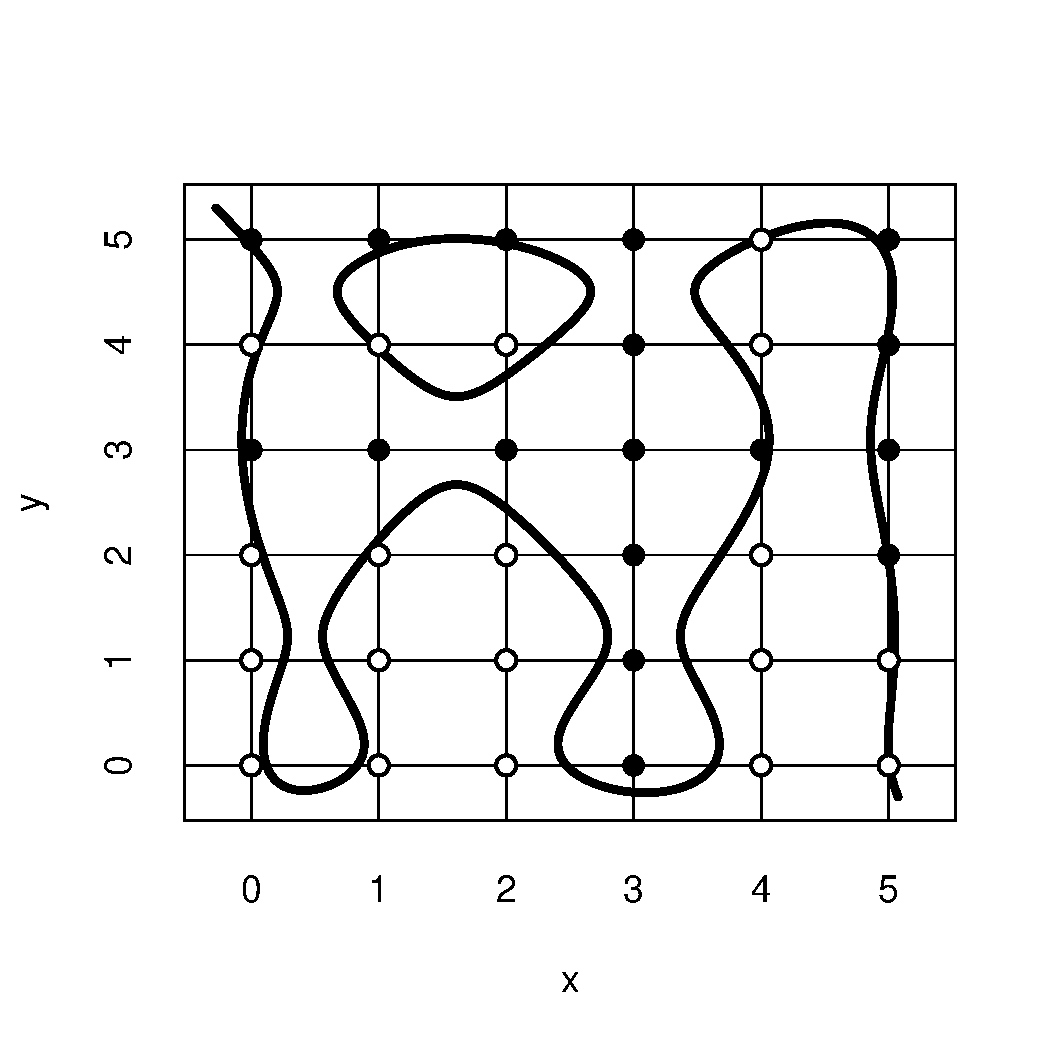
\includegraphics[scale=0.4]{nb1}
\caption{ $X,Y \in \{0,1,\ldots,5\}$} 
\end{subfigure}
\begin{subfigure}[b]{0.45\textwidth}
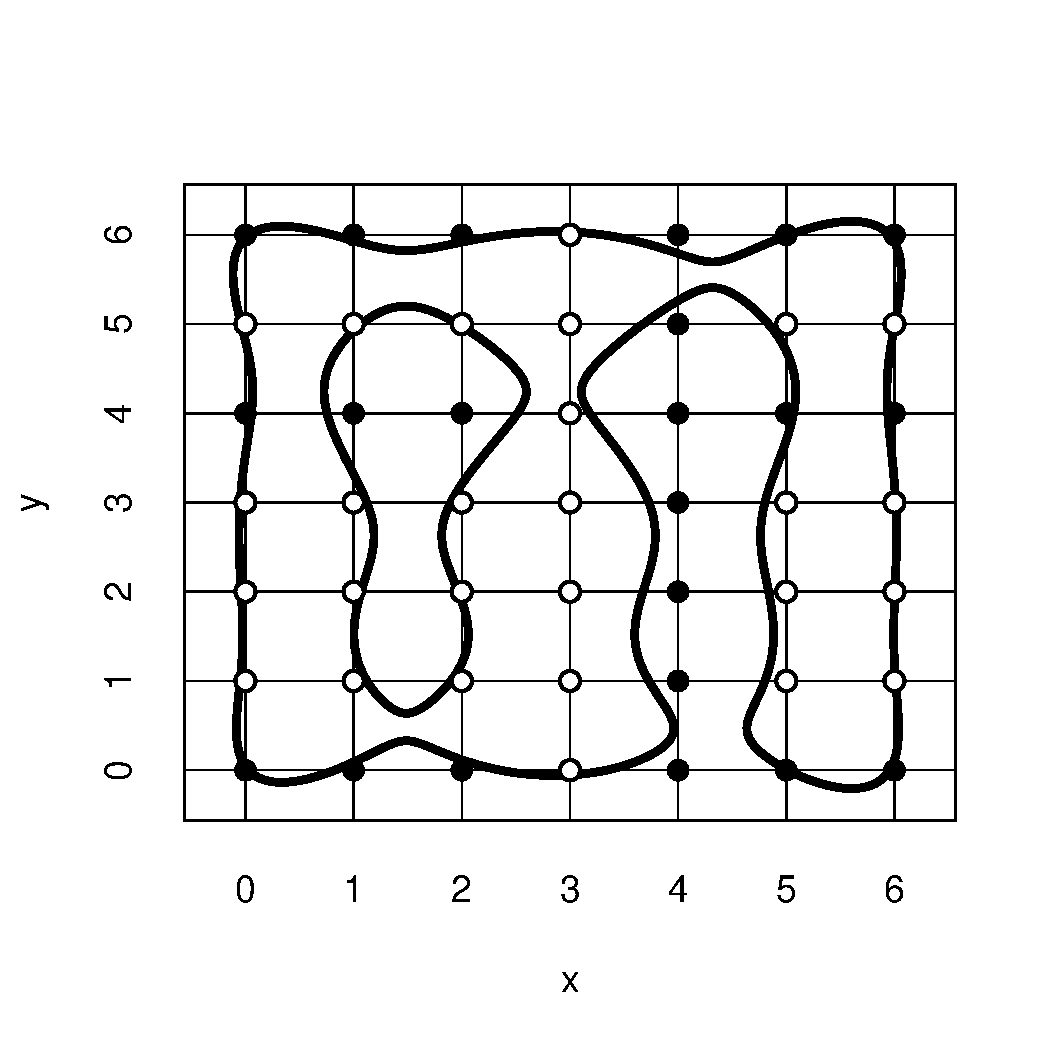
\includegraphics[scale=0.4]{nb2}
\caption{ $X,Y \in \{0,1,\ldots,6\}$}
\end{subfigure}
%\begin{subfigure}[b]{0.3\textwidth}
%\includegraphics[scale=0.24]{fig7point}
%\caption{ $X,Y \in \{0,1,\ldots,7\}$}
%\end{subfigure}
\caption{Decision boundary for {two example}, (a) and (b), of naive Bayes classifiers with two categorical variables $X$, $Y$. {Boundaries are computed as location of zeroes of polynomials built as in Theorem \ref{teo: NB categorical}}}
\label{fig:decboundfig}
\end{figure}
\begin{theorem}
{A discrimination function $f \in\mathcal{F}$ for a binary classification problem} over $n$ categorical variables $X_i \in \nchi_i=\{\xi_i^1,\ldots,\xi_i^{m_i}\}$, with $|\nchi_i|=m_i$, is equal over $\bchi$ to a polynomial of the form $\sum_{i=1}^n \left( \sum_{j=1}^{m_i}  \alpha_{i}(j)\ell ^{\nchi_i} _j(x_i) \right)$ if and only if there exists a naive Bayes classifier, {with probability tables without zeros entries}, that induces $f$, where $\ell_j^{\nchi_i}$ are the Lagrange basis over $\nchi_i$.
\label{teo: NB categorical}
\end{theorem}
\begin{proof}
We consider a naive Bayes classifier as in Figure \ref{fig:NB}. For every $i \in [n]$ the variable $X_i$ takes values over $\nchi_i=\{\xi_i^1,\ldots,\xi_i^{m_i}\}$,  a subset of $\mathbb{R}$ of cardinality $m_i$.
Thanks to Equation (\ref{eq:lagrange prob interp}), we can express, for every value $c$ of the class, the conditional probability $\Pp(X_i | C)$ as 
\[ \Pp(X_i=x_i | C=c)=\prod_{j=1}^{m_i} p_{i}(j|c)^{\ell ^{\nchi_i} _j(x_i)} , \]
where $p_{i}(j|c)=\Pp(X_i=\xi_i^j|C=c)$.
If we define $a_{i}(j|c)=\log ( p_{i}(j|c) )$, and assuming that $p_{i}(j|c)> 0$, we have that
\begin{equation}
\label{eq:prob espon}
 \Pp(X_i=x_i | C=c)=\exp \left( \sum_{j=1}^{m_i} a_{i}(j|c)\ell ^{\nchi_i} _j(x_i)\right). 
 \end{equation}
Using this representation we easily find the induced discrimination function for the NB with arbitrary discrete predictor variables.
Setting $a=\log ( \Pp(C=+1) ) $ and $b=\log ( \Pp(C=-1) ) $, we have that 
\[ f_{\Pp}(\bx)= \log\left(\Pp(X_1=x_1,\ldots,X_n=x_n,C=+1)\right)- \left(\Pp(X_1=x_1,\ldots,X_n=x_n,C=-1)\right) . \]
Using Equations (\ref{eq:fact NB}) and (\ref{eq:prob espon}) we have that 
\[  f_{\Pp}(\bx)= \left( a+ \sum_{i=1}^n \left( \sum_{j=1}^{m_i}  a_{i}(j|+1)\ell ^{\nchi_i} _j(x_i) \right) \right) -  \left( b+ \sum_{i=1}^n \left( \sum_{j=1}^{m_i}  a_{i}(j|-1)\ell ^{\nchi_i} _j(x_i) \right) \right) , 
\]
so the discrimination function for a naive Bayes classifier is  
\begin{equation}
\label{eq:DB NB general}
f^{NB}(\mathbf{x})= a-b + \sum_{i=1}^n \left( \sum_{j=1}^{m_i} \alpha'_{i}(j)\ell ^{\nchi_i} _j(x_i) \right)  ,
\end{equation}
where ${\alpha'}_{i}(j)=a_{i}(j|+1)-a_{i}(j|-1)=\log \left( \frac{\Pp(X_i=\xi_i^j|C=+1)}{\Pp(X_i=\xi_i^j|C=-1)} \right)$.
We see from Equation (\ref{eq:DB NB general}) that the decision function is sign-represented by a polynomial that admits the representation $\sum_{i=1}^n \left( \sum_{j=1}^{m_i}  \alpha_{i}(j)\ell ^{\nchi_i} _j(x_i) \right)$. {In fact we have that the $a-b=\log\left(\frac{\Pp(C=+1)}{\Pp(C=-1)}\right)$ term could be included in the summation using Lemma \ref{lem:LAG}, for example with the following choice of coefficient},
\begin{equation}
{
\alpha_{i}(j)=\log \left( \frac{\Pp(X_i=\xi_i^j|C=+1)}{\Pp(X_i=\xi_i^j|C=-1)} \right)+k_i\log \left( \frac{\Pp(C=+1)}{\Pp(C=-1)} \right),}
\label{eq:coefalpha}
\end{equation} 
{where $\sum_{i=1}^n k_i=1$.}
We have proved the \textit{if} part of the theorem.  

To prove the \textit{only if} we have just to observe that choosing the conditional probabilities for the predictor variables given the class, $\Pp(X_i=\xi_i^j|C=c)$, the probability mass for the class $\Pp(C=+1)=1-\Pp(C=-1)$, and the values of $\{k_i\}_{i=1}^n$ we are able to adjust the coefficients $\alpha_i(j)$ in (\ref{eq:coefalpha}) to any possible values in $\mathbb{R}$.
For example the following choices are sufficient
\begin{align*}
&\Pp(X_i=\xi_i^j|C=-1)=\frac{1}{m_i}\quad \forall i \in [n] \text{ and } j=1,\ldots,m_i ,\\
&\Pp(X_i=\xi_i^j|C=+1)=\frac{e^{\alpha_i(j)}}{\sum_{j=1}^{m_i}e^{\alpha_i(j)}} \quad \forall i \in [n] \text{ and } j=1,\ldots,m_i,\\
&k_i= \frac{\log\left( \frac{1}{m_i}\sum_{j=1}^{m_i}e^{\alpha_i(j)} \right)}{\sum_{i=1}^n \log\left(\frac{1}{m_i} \sum_{j=1}^{m_i}e^{\alpha_i(j)}\right)} \quad \forall i \in [n] ,\\
&\log\left( \frac{\Pp(C=+1)}{\Pp(C=-1)} \right)=\sum_{i=1}^n \log\left( \frac{1}{m_i}\sum_{j=1}^{m_i}e^{\alpha_i(j)} \right).  
\end{align*} 
\end{proof}

As a result of Theorem \ref{teo: NB categorical} we have that a naive Bayes classifier could represent every decision function which is sign-representable by a polynomial of the family 
\[ \mathcal{F}_{NB}=\left\{ r(\mathbf{x})=\sum_{i=1}^n \left( \sum_{j=1}^{m_i}  \alpha_{i}(j)\ell ^{\nchi_i} _j(x_i) \right)\text{, } \alpha_{i}(j) \in \mathbb{R}  \right\} . \]


Only if we fix the prior probability over the class $C$ there are restrictions on the coefficients $\alpha_{i}(j)$. 

\begin{corollary}
Let $f \in \mathcal{F}$ be a discrimination function for a binary classification problem with $n$ categorical predictor variables $X_i \in \nchi_i=\{\xi_i^1,\ldots,\xi_i^{m_i}\}\subset \mathbb{R}$. The following sentences are equivalent:
\begin{enumerate}
\item[i)] $f$ is equal over $\bchi$ to a polynomial of the form $\sum_{i=1}^n \left( \sum_{j=1}^{m_i}  \alpha_{i}(j)\ell ^{\nchi_i} _j(x_i) \right)$ with $\alpha_{i}(j)$ such that for every $i=1,\ldots,n$, there exists $j_{i,1}$ and $j_{i,2}$ such that ${\alpha_{i}(j_{i,1})}<0$ and ${\alpha_{i}(j_{i,2})}>0$ or alternatively $e^{\alpha_{i}(j)}=1$ for every $j=1,\ldots,m_i$.   
\item[ii)] There exists a naive Bayes classifier, {with probability tables without zeros entries} and with uniform prior probability over the class $C$, that induces $f$.
\end{enumerate}
\label{cor: NB categorical prior}
\end{corollary}
\begin{proof}
The corollary follows from (\ref{eq:coefalpha}) in proof of Theorem \ref{teo: NB categorical}, it is easy to show that the two conditions are equivalent.
\end{proof}

As we can see, the coefficients $\alpha_i(j)$ are related to the probability model underlying the problem, and are usually estimated from the training set but they do not generally assure the minimization of classification errors.
An interesting model to deal with this problem is the weighted naive Bayes classifier \citep{Webb98,Hall2007}. Weights are introduced in the probability factorization,  
\[ \Pp(C=c|\mathbf{X}=\mathbf{x}) \propto w_c\Pp(C=c)\prod_{i=1}^{n} \left[ \Pp(X_i=x_i|C=c)\right]^{w_i} ,\]
and thus the decision function has the same form as in Equation (\ref{eq:DB NB general}), but with modified coefficients
\[ \alpha_{i}(j)= w_i \log \frac{\Pp(X_i=j|C=+1)}{\Pp(X_i=j|C=-1)} .\]
Note that introducing the weights in the model does not change the form of the polynomial sign-representing the decision functions, so it does not improve the expressive power of the model. Even so, using the weighted model it is possible to search for polynomials that minimize the misclassification and improve accuracy \citep{zaidi13}. 
%As future research it may be of some interest to study how to search polynomials to directly minimize the misclassification error and how this reflects on the implicitly defined NB classifier.

\begin{example}
\label{exp:1}
We consider a naive Bayes classifier with two predictor variables $X_1 \in \nchi_{1}=\{0,1,2,3,4\}$ and $X_2 \in \nchi_{2}=\{0,1,2\}$.
We have a uniform prior probability over the class $C$, that is, $\Pp(C=-1)=\Pp(C=+1)=0.5$, and we consider the  conditional probability tables for $X_1$ and $X_2$ given in Table \ref{tab:condprob1}.
\begin{table}
\centering

  \begin{tabular}{llll}

    \begin{tabular}{|l|l|l|}
    \hline
    $X_1$ & $C=-1$ & $C=+1$ \\ \cline{1-3}
    $0$ & $0.3$    & $0.3$    \\ \cline{1-3}
    $1$ & $0.1$    & $0.2$    \\ \cline{1-3}
    $2$ & $0.4$    & $0.1$    \\ \cline{1-3}
    $3$ & $0.1$    & $0.2$    \\ \cline{1-3}
    $4$ & $0.1$    & $0.2$    \\ \cline{1-3}
    \end{tabular}
    & & &

    \begin{tabular}{|l|l|l|}
    \hline
    $X_2$ & $C=-1$ & $C=+1$ \\ \hline
    $0$ & $0.2$    & $0.4$    \\ \hline
    $1$ & $0.1$    & $0.2$    \\ \hline
    $2$ & $0.7$    & $0.4$    \\ \hline
    \end{tabular}

 \end{tabular}
 \caption{Conditional probability tables in Example \ref{exp:1}}
\label{tab:condprob1}
\end{table}
We can directly build the polynomial threshold functions $r(x_1,x_2)$ that sign-represent the decision function induced by this classifier.
The related coefficients are $\alpha_{1}(j)=\log \frac{ \Pp(X_1=j|C=+1)}{\Pp(X_1=j|C=-1)}$ and $\alpha_{2}(j)=\log \frac{ \Pp(X_2=j|C=+1)}{\Pp(X_2=j|C=-1)}$, and the polynomial $r(x_1,x_2)$ is
\begin{equation} \label{eq:pol1} r(x_1,x_2)=\sum_{j=0}^{4} \alpha_1(j)\ell_{j}^{\nchi_1}(x_1)+\sum_{j=0}^{2} \alpha_2(j)\ell_{j}^{\nchi_2}(x_2).  \end{equation}
The computations of the coefficients are shown in Table \ref{tab:coefficients}.
\begin{table}
\centering
 \begin{tabular}{|l|l|}
\hline
& \\
$\alpha_1(0)=\log \frac{0.3}{0.3}=0$  &   $\alpha_2(0)=\log \frac{0.4}{0.2}=\log2 $
\\ & \\
$\alpha_1(1)=\log \frac{0.2}{0.1}=\log2$ &  $\alpha_2(1)=\log \frac{0.2}{0.1}=\log2$ 
\\ & \\
$\alpha_1(2)=\log \frac{0.1}{0.4}=-\log4$ &  $\alpha_2(2)=\log \frac{0.4}{0.7}=-\log\frac{7}{4} $
\\ & \\
$\alpha_1(3)=\log \frac{0.2}{0.1}=\log2$ &  
\\ & \\
$\alpha_1(4)=\log \frac{0.2}{0.1}=\log2$  &  \\
& \\
\hline
\end{tabular}  
\caption{{Coefficient computations of the polynomial in Equation (\ref{eq:pol1})} }
\label{tab:coefficients}
\end{table}
We have that the polynomial threshold function in Equation (\ref{eq:pol1}), expressed with the Lagrange basis, is
\begin{align*}
r(x_1,x_2)=& \frac{x_1(x_1-2)(x_1-3)(x_1-4)}{-6}\log2- \frac{{x_1}(x_1-1)(x_1-3)(x_1-4)}{4}\log4 \\
 &{}+\frac{x_1(x_1-1)(x_1-2)(x_1-4)}{-6}\log2+\frac{x_1(x_1-1)(x_1-2)(x_1-3)}{24}\log2 \\ 
 &{}+\frac{(x_2-1)(x_2-2)}{2}\log2+ \frac{x_2(x_2-2)}{-1} \log2-\frac{x_2(x_2-1)}{2}\log\frac{7}{4}. 
\end{align*}
We observe that the above polynomial satisfies the condition of {Corollary} \ref{cor: NB categorical prior}, as it should because the prior probability over $C$ is uniform. 
Figure \ref{fig:exp1} shows the decision boundary induced by $r(x_1,x_2)$.
\begin{figure}
\centering
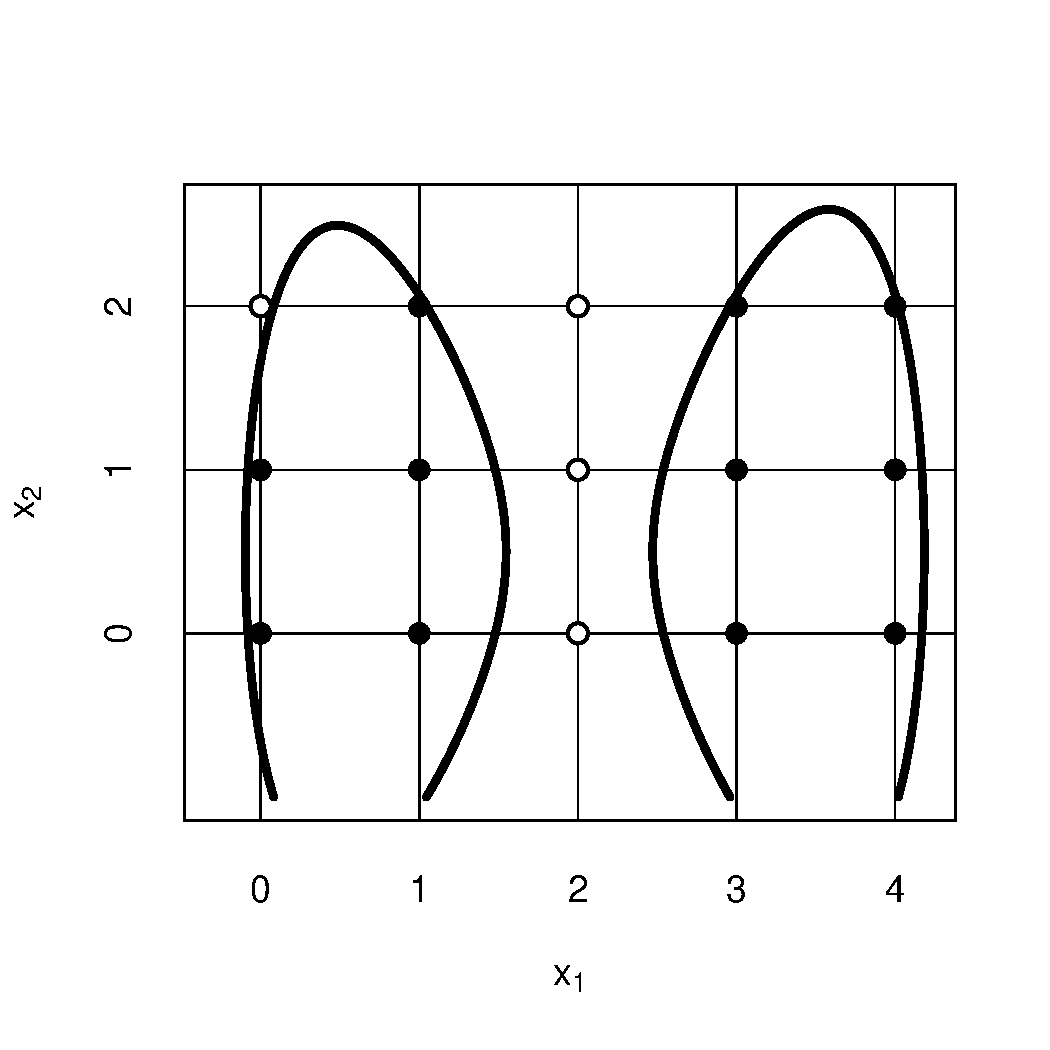
\includegraphics[scale=0.65]{nbexample}
\caption{Decision boundary for the naive Bayes structure of Example \ref{exp:1}}
\label{fig:exp1}
\end{figure}
\end{example}

\subsection{Tree Augmented Naive Bayes}
\label{subsec:TAN}
\begin{figure}
\centering
\begin{tikzpicture}[->,>=stealth',shorten >=1pt,auto,node distance=3cm,
  thick,main node/.style={circle,fill=white!20,draw,font=\sffamily\Large\bfseries},minimum width=1.5cm]
  
  \node[main node] (1) {$C$};
  \node[main node] (6) [below of=1] {$X_3$};
  \node[main node] (3) [left of=6] {$X_2$};
  \node[main node] (2) [left of=3] {$X_1$};  
  \node[main node] (4) [right of=6] {$X_{4}$};
  \node[main node] (5) [right of=4] {$X_{5}$};

  
  \path[every node/.style={font=\sffamily\small}]
    (1) edge node [left] {}  (2)
        edge node[left] {} (3)
        edge node[left] {} (4)
        edge node[left] {} (6)
        edge node[left] {} (5)
    (2) edge node [left] {} (3)
        edge [bend right] node [left] {} (6)
    (6) edge node [left] {} (4)        
    (4) edge node [left] {} (5);
  
\end{tikzpicture}  
\caption{Tree augmented naive Bayes classifier structure with five predictor variables}
\label{fig:TAN}
\end{figure}
We now consider a tree augmented naive Bayes (TAN) classifier \citep{Friedman1997} as shown in Figure \ref{fig:TAN}. In this model, a predictor variable $X_i\in \nchi_i=\{\xi_i^1,\ldots,\xi_i^{m_i}\}$ is allowed to have at most two parents, the class $C$ and an other variable, $X_{pa(i)}\in \nchi_{pa(i)}$.     
The joint probability distribution of $(C,X_1,X_2,\ldots ,X_n)$ over $\{-1,+1\}\times\nchi_1\times\cdots\times\nchi_n$ can be factorized according to the Bayesian network theory as
\begin{equation} \Pp\left(C=c\right)\prod_{i=1}^n \Pp\left(X_i=x_i|C=c, X_{pa(i)}=x_{pa(i)}\right) .\label{eq:tan fact}  \end{equation}
We can write down a similar representation to the NB case.
For each $i=1, \ldots,n$, we apply Equation (\ref{eq:lagrange prob interp cond}) and obtain 
\begin{equation}
\label{eq:conprob}
\Pp\left( X_i=x_i|C=c,X_{pa(i)}=x_{pa(i)} \right)=\prod_{j=1}^{m_i}\prod_{k=1}^{m_{pa(i)}}p_{i}(j|c,k)^{ \left( \ell_{k}^{\nchi_{pa(i)}}(x_{pa(i)})  \ell_{j}^{\nchi_i}(x_i) \right) }.
\end{equation}
We can now prove, combining Equations (\ref{eq:tan fact}) and (\ref{eq:conprob}), a result similar to the NB case.
\begin{lemma}
\label{lem:TANteo}
If $f^{TAN}$ is the discrimination function induced by a TAN for a binary classification problem with $n$ categorical predictor variables $\{X_i \in \nchi_i \}_{i=1}^n${ and  with probability tables without zeros entries}, then there exists a polynomial, of the form 
\[ \sum_{i=1}^{n}  \sum_{j=1}^{m_i} \ell_{j}^{\nchi_i}(x_i) \sum_{k=1}^{m_{pa(i)}} \beta_{i}(j|k)\ell_{k}^{\nchi_{pa(i)}}(x_{pa(i)}) ,  \]
that interpolates $f^{TAN}$ over $\bchi$, where we consider $\sum_{k=1}^{m_{pa(i)}} \beta_{i}(j|k)\ell_{k}^{\nchi_{pa(i)}}(x_{pa(i)})=\beta_{i}(j)$  when $\nchi_{pa(i)}=\emptyset$, that is, when class $C$ is the only parent of a node (the root node of the tree).
\end{lemma} 
\begin{proof}
The proof is a straightforward computation of the logarithm of Equation (\ref{eq:tan fact}) using Equation (\ref{eq:conprob}) and the definition  $\beta_{i}(j|k)=\log\left(\frac{p_{i}(j|+1,k)}{p_{i}(j|-1,k)}\right)$. The term corresponding to the probability over the class $\log \left( \frac{\Pp(C=+1)}{\Pp(C=-1)}\right)$ could be made vanishing into the coefficients of the root node $X_t$ of the tree, using point 2 of Lemma \ref{lem:LAG} with $I=\{t\}$, with the following choice of coefficients
$$ \beta_t(j)=\log\left(\frac{p_{i}(j|+1)}{p_{i}(j|-1)}\right)+\log \left( \frac{\Pp(C=+1)}{\Pp(C=-1)}\right).$$
\end{proof}
\begin{figure}
\centering
\begin{tikzpicture}[->,>=stealth',shorten >=1pt,auto,node distance=3cm,
  thick,main node/.style={circle,fill=white!20,draw,font=\sffamily\Large\bfseries},minimum width=1.5cm]
  
  \node[main node] (1) {$C$};
  \node[main node] (8) [below  of=1] {$X_{sp}$};
  \node[main node] (3) [below left of=1] {$X_2$};
  \node[main node] (2) [left of=3] {$X_1$};  
  \node[main node] (4) [below right of=1] {$X_{3}$};
  \node[main node] (5) [right of=4] {$X_{4}$};
  
  \path[every node/.style={font=\sffamily\small}]
    (1) edge node [left] {}  (2)
        edge node[left] {} (3)
        edge node[left] {} (4)
        edge node[left] {} (5)
        edge node[left] {} (8)
    (8) edge node [left] {} (3)
    (8) edge node [left] {} (4)
    (8) edge [bend left] node [left] {} (2)
    (8) edge [bend right] node [left] {} (5);    
  
  
\end{tikzpicture}  
\caption{SPODE Bayes classifier structure with five predictor variables}
\label{fig:SPODE}
\end{figure}

A particular case of TAN is the \textit{SuperParent-One-Dependence Estimator} (SPODE) \citep{keogh2002}, where all the predictors depend on the same predictor (superparent) (Figure \ref{fig:SPODE}). The joint distribution factorizes as follows:
\[ \Pp\left(C=c\right)\Pp\left(X_{sp}=x_{sp}|C=c\right)\prod_{i\neq sp} \Pp\left(X_i=x_i|C=c, X_{sp}=x_{sp}\right), \]
where $X_{sp}$ stands for the superparent node.
In this case, the representation of Lemma \ref{lem:TANteo} reduces to
\begin{equation}
\label{eq:superparent}
f^{SPODE}(\mathbf{x})= sign\left(  \sum_{i\neq sp} \sum_{j=1}^{m_i}\ell_j^{\nchi_i}(x_i) \sum_{k=1}^{m_{sp}} \beta_{i}(j|k) \ell_k^{\nchi_{sp}}(x_{sp})\right)   ,
\end{equation} 
where $f^{SPODE}$ is the induced discrimination function.
If we fix the superparent node, we have a stronger characterization of the induced discrimination functions, the analogue of Theorem \ref{teo: NB categorical}.
\begin{theorem}
\label{teo:SPODE}
A discrimination function for a binary classification problem over categorical predictor variables is interpolated by a polynomial of the form   \[\sum_{i\neq sp} \sum_{j=1}^{m_i}\ell_j^{\nchi_i}(x_i)\sum_{k=1}^{m_{sp}} \beta_{i}(j|k) \ell_k^{\nchi_{sp}}(x_{sp}),\] if and only if it is induced by a SPODE classifier with $X_{sp}$ as the superparent node { and  with probability tables without zeros entries}.
\end{theorem}
\begin{proof}
The \textit{if} part of the theorem is precisely Equation (\ref{eq:superparent}). To prove the \textit{only if} part we repeat a similar argument as in Theorem \ref{teo: NB categorical}.
We observe (Lemma \ref{lem:LAG}, point 4, with $J=\{i\}$ and $I=\{i,sp\}$) that for every $i\neq sp$,
\[ \ell_k^{\nchi_{sp}}(x_{sp})=\sum_{j=1}^{m_i} \ell_j^{\nchi_i}(x_i) \ell_k^{\nchi_{sp}}(x_{sp}), \] 
and so the coefficient $\beta_i(j|k)$ could be seen as 
\[ \beta_i(j|k)=\log\left( \frac{ \Pp( X_i=j|X_{sp}=k, C=+1)}{\Pp( X_i=j|X_{sp}=k, C=-1)} \right) + \alpha_i(k),  \]
where $ \sum_{i\neq sp} \alpha_{i}(k) = \log\left( \frac{\Pp(X_{sp}=\xi_{sp}^k|C=+1}{\Pp(X_{sp}=\xi_{sp}^k|C=-1} \right) + \alpha $ and $\alpha=\log\left( \frac{\Pp(C=+1)}{\Pp(C=-1)} \right)$.
Then adjusting $\alpha_i(k)$ and $\alpha$ properly we can find a SPODE model, that is, probability distributions over the predictors and the class that induces 
\[f=   \sum_{i\neq sp} \sum_{j=1}^{m_i}\ell_j^{\nchi_i}(x_i)\sum_{k=1}^{m_{sp}} \beta_{i}(j|k) \ell_k^{\nchi_{sp}}(x_{sp}) , \]
for every $\beta_i(j|k) \in \mathbb{R}$.
\end{proof}
\begin{remark}  \label{rmrk:1}
We observe that, as for Theorem \ref{teo: NB categorical}, the proof of Theorem \ref{teo:SPODE} adds \textit{free} parameters to the model. For every variable we modify the related coefficients and then we adjust the modifications with the parent coefficients. As in the proof of Theorem \ref{teo: NB categorical} we are able to use the added parameters to define proper probability distributions, that is to make the defined probability add up to one.   \end{remark}
\begin{remark}  \label{rmrk:2}
Results similar to Theorem \ref{teo:SPODE} could be proved whenever the structure of the predictor subgraph of a TAN classifier is fixed. We expound no further theorems about TAN classifiers, as, in the next section, we will prove a more general result, of which NB and TAN are special cases.    \end{remark}
\begin{example}
\label{exp:2}
We look at the SPODE model (see Figure \ref{fig:exmpl SPODE} for structure) with the superparent node $X_{sp}$.
\begin{figure}[p]
\centering
\begin{tikzpicture}[->,>=stealth',shorten >=1pt,auto,node distance=3cm,
  thick,main node/.style={circle,fill=white!20,draw,font=\sffamily\Large\bfseries},minimum width=1.5cm]
  
  \node[main node] (1) {$C$};
  \node[main node] (2) [below  of=1] {$X_{sp}$};
  \node[main node] (3) [below left of=1] {$X_1$}; 
  \node[main node] (4) [below right of=1] {$X_{2}$};

  
  \path[every node/.style={font=\sffamily\small}]
    (1) edge node [left] {}  (2)
        edge node[left] {} (3)
        edge node[left] {} (4)
    (2) edge node [left] {} (3)
    (2) edge node [left] {} (4);
   
  
  
\end{tikzpicture}  
\caption{SPODE classifier structure, Example \ref{exp:2}}
\label{fig:exmpl SPODE}
\end{figure}
We consider $X_1 \in \{0,1,2\}$, $X_2 \in \{0,1,2,3\}$ and $X_{sp}\in \{0,1\}$ with  conditional probability tables as shown in Table \ref{tab:cond tab 2}.
\begin{table}[p]
\centering
  \begin{tabular}{c}
  
    \begin{tabular}{|l|l|l|}
    \hline
    $X_{sp}$ & $C=-1$ & $C=+1$ \\ \cline{1-3}
    $0$ & $0.8$    & $0.4$    \\ \cline{1-3}
    $1$ & $0.2$    & $0.6$    \\ \cline{1-3}
    \end{tabular}
  
    
    \begin{tabular}{|l|l|l|l|l|}
    \hline
    $X_1$ & \multicolumn{2}{c|}{$C=-1$}  & \multicolumn{2}{c|}{$C=+1$ }   \\ \cline{1-5}
        &  $X_{sp}=0$  &  $X_{sp}=1$ &  $X_{sp}=0$  &  $X_{sp}=1$  \\ \hline    
    $0$ & $0.1$  & $0.3$ & $0.2$ & $0.7$    \\ \hline
    $1$ & $0.1$  & $0.2$ & $0.7$ & $0.1$    \\ \hline
    $2$ & $0.8$  & $0.5$ & $0.1$ & $0.2$    \\ \hline
    \end{tabular}
    
 \\   \\
     \begin{tabular}{|l|l|l|l|l|}
    \hline
    $X_2$ & \multicolumn{2}{c|}{$C=-1$}  & \multicolumn{2}{c|}{$C=+1$ }   \\ \cline{1-5}
        &  $X_{sp}=0$  &  $X_{sp}=1$ &  $X_{sp}=0$  &  $X_{sp}=1$  \\ \hline    
    $0$ & $0.5$  & $0.5$ & $0.5$ & $0.2$    \\ \hline
    $1$ & $0.2$  & $0.2$ & $0.3$ & $0.2$    \\ \hline
    $2$ & $0.1$  & $0.2$ & $0.1$ & $0.5$    \\ \hline
    $3$ & $0.2$  & $0.1$ & $0.1$ & $0.1$    \\ \hline
    \end{tabular}
 \end{tabular}
 \caption{Conditional probability tables in Example \ref{exp:2} }
 \label{tab:cond tab 2}
\end{table}
The polynomial threshold function $r(x_{sp},x_1,x_2)$ can be computed directly as specified in Lemma \ref{lem:TANteo}:
\begin{align*}
r&(x_sp,x_1,x_2)= (1-x_{sp})\log\left(\frac{0.4}{0.8}\right)+x_{sp}\log\left(\frac{0.6}{0.2}\right) \\
&+(1-x_{sp})\left( \frac{(1-x_1)(2-x_1)}{2}\log\left(\frac{0.2}{0.1}\right) + x_1(2-x_1)\log\left(\frac{0.7}{0.1}\right)+\frac{x_1(x_1-1)}{2}\log\left(\frac{0.1}{0.8}\right) \right) \\
&+x_{sp}\left( \frac{(1-x_1)(2-x_1)}{2}\log\left(\frac{0.7}{0.3}\right) + x_1(2-x_1)\log\left(\frac{0.1}{0.2}\right)+\frac{x_1(x_1-1)}{2}\log\left(\frac{0.2}{0.5}\right) \right) \\
&+(1-x_{sp})\left(  \frac{x_2(2-x_2)(3-x_2)}{2}\log\left(\frac{0.3}{0.2}\right) + \frac{x_2(x_2-1)(x_2-2)}{6}\log\left(\frac{0.1}{0.2}\right)  \right)\\
&+x_{sp}\left(  \frac{(1-x_2)(2-x_2)(3-x_2)}{6}\log \left(\frac{0.2}{0.5}\right) + \frac{x_2(x_2-1)(3-x_2)}{2}\log\left(\frac{0.5}{0.2} \right) \right) .
\end{align*}
We observe that some elements of the Lagrange bases do not appear in $r(x_{sp},x_1,x_2)$ because the corresponding coefficients are zero, since the conditional probabilities given $C$ are equal.
\end{example}

\subsection{Bayesian Network-Augmented Naive Bayes}
\label{subsec:BAN}
If the predictor subgraph can be a generic Bayesian network, we have a Bayesian network-augmented naive Bayes (BAN) classifier. In this case the joint probability distribution is factorized as follows:
\begin{equation}
\label{eq:BAN fact}
\Pp\left(C=c\right)\prod_{i=1}^n \Pp\left(X_i=x_i|C=c, \mathbf{X}_{{pa}(i)}=\mathbf{x}_{{pa}(i)}\right) ,
\end{equation}
where $\mathbf{X}_{{pa}(i)}$ denotes the vector of the parent variables of $X_i$ that are not $C$. 
From now on for BAN classifiers we will write ${pa}(i)$ for the set of indexes defining $X_i$'s parents that are not $C$ and $\mathbb{M}_i=\times_{s\in {pa}(i)} \{1,\ldots,m_s\} $ for the set of possible configurations of the parents of $X_i$.
Applying the same arguments as in previous sections  we can prove the lemma below.
\begin{lemma}
\label{lem:BAN}
If $f^{BAN}$ is the discrimination function induced by a BAN classifier for a {binary} classification problem with $n$ categorical predictors variables $\{X_i \in \nchi_i\subset\mathbb{R} \text{, } |\nchi_i|=m_i\}_{i=1}^n$ { and  with probability tables without zeros entries}, then there exists a polynomial of the form 
\[ \sum_{i=1}^{n}  \sum_{j=1}^{m_i}\ell_{j}^{\nchi_i}(x_i) \sum_{\mathbf{k}\in \mathbb{M}_i} \beta_{i}(j|\mathbf{k})\prod_{s\in {pa}(i)} \ell_{k_s}^{\nchi_{s}}(x_{s}) ,  \]
which interpolates $f^{BAN}$, where we write $\sum_{\mathbf{k}\in \mathbb{M}_i} \beta_{i}(j|\mathbf{k})\prod_{s\in {pa}(i)} \ell_{k_s}^{\nchi_{s}}(x_{s})=\beta_{i}(j)$ when a variable does not have parents that are not $C$, that is, ${pa}(i)=\emptyset$.
\end{lemma}
\begin{proof}
Given a BAN model over predictors $X_i \in \nchi_i=\{\xi_i^1,\ldots,\xi_i^{m_i}\}$, we define 
\[ \beta_{i}(j|\mathbf{k})=\log \left( \frac{P\left(X_i=\xi_i^j|C=+1, X_s=\xi_s^{k_s} \text{, } \forall s\in {pa}(i)  \right) }{P\left(X_i=\xi_i^j|C=-1, X_s=\xi_s^{k_s} \text{, }\forall s\in {pa}(i)  \right)} \right) .\]
Using Equation (\ref{eq:lagrange prob interp cond}) and taking the logarithm of Equation (\ref{eq:BAN fact}) we obtain the polynomial representation. The additional constant term due to the prior probability over the class, $\log \left( \frac{\Pp(C=+1)}{\Pp(C=-1)}\right)$, could be embedded into the $\beta_i(j|\mathbf{k})$ coefficients using point 2 of Lemma \ref{lem:LAG} as in the proofs of Theorem \ref{teo: NB categorical} and Lemma \ref{lem:TANteo}.
\end{proof}



Generally speaking, it is not always possible to prove results similar to Theorem \ref{teo: NB categorical} or Theorem \ref{teo:SPODE} for BAN classifiers, when discrimination functions are completely characterized by sets of polynomials. Like \citet{Yang2012}, we find that problems arise in the presence of $V$-structures (Figure \ref{fig:Vstr}) in the predictor subgraph. 

In absence of $V$-structures we can prove the following result, which extends the previous ones.
\begin{theorem}
\label{teo:BAN}
Let $\mathcal{G}$ be a directed acyclic graph with node $X_i$ for $i=1,\ldots,n$, and let $f \in\mathcal{F}$ be a discrimination function {for a binary classification problem} over predictor variables $X_i \in \nchi_i=\{\xi_i^1,\ldots,\xi_i^{m_i}\}$. Suppose that $\mathcal{G}$ does not contain $V$-structures, then we have that $f$ is interpolated by the following polynomial 
\[ r(\mathbf{x})=\sum_{i=1}^{n} \sum_{j=1}^{m_i}\ell_{j}^{\nchi_i}(x_i) \sum_{\mathbf{k}\in \mathbb{M}_i} \beta_{i}(j|\mathbf{k})\prod_{s\in {pa}(i)} \ell_{k_s}^{\nchi_{s}}(x_{s}) ,\] 
if and only if $f$ is induced by a BAN classifier whose predictor subgraph is $\mathcal{G}$ { and  with probability tables without zeros entries}.
\end{theorem}
\begin{proof}
We merely have to prove the \textit{only if} because the \textit{if} implication is precisely Lemma \ref{lem:BAN}.
Given a polynomial of the form
\[ r(\mathbf{x})=\sum_{i=1}^{n} \sum_{j\in\nchi_i}\ell_{j}^{\nchi_i}(x_i) \sum_{\mathbf{k}\in \mathbb{M}_i} \beta_{i}(j|\mathbf{k})\prod_{s\in {pa}(i)} \ell_{k_s}^{\nchi_{s}}(x_{s}) ,\] 
we have to find a BAN classifier inducing $r(\mathbf{x})$, whose predictor subgraph is $\mathcal{G}$. We just have to define the conditional probability distribution of every variable given its parents, since the structure of the BAN is already fixed by $\mathcal{G}$.
For every $i=1,\ldots,n$, we observe that the subgraph of the parents of $X_i$ is a fully connected Bayesian network, otherwise we will have a $V$-structure on $\mathcal{G}$.
For every $i$, we can rewrite using point 4 of Lemma \ref{lem:LAG} the $i$-th addend on the summation,
\begin{align*}
 &\sum_{j\in\nchi_i}\ell_{j}^{\nchi_i}(x_i) \sum_{\mathbf{k}\in \mathbb{M}_i} \beta_{i}(j|\mathbf{k})\prod_{s\in {pa(i)}} \ell_{k_s}^{\nchi_{s}}(x_{s}) + \sum_{\mathbf{k}\in \mathbb{M}_i} \alpha_i(\mathbf{k})\prod_{s\in {pa}(i)} \ell_{k_s}^{\nchi_{s}}(x_{s}) - \sum_{\mathbf{k}\in \mathbb{M}_i} \alpha_i(\mathbf{k})\prod_{s\in {pa}(i)} \ell_{k_s}^{\nchi_{s}}(x_{s}) \\
 =&\sum_{j \in \nchi_i}\ell_{j}^{\nchi_i}(x_i) \sum_{\mathbf{k}\in \mathbb{M}_i} \left( \beta_{i}(j|\mathbf{k})+\alpha_i(\mathbf{k}) \right)\prod_{s\in  {pa}(i)} \ell_{k_s}^{\nchi_{s}}(x_{s}) -\sum_{\mathbf{k}\in \mathbb{M}_i} \alpha_i(\mathbf{k})\prod_{s\in {pa}(i)} \ell_{k_s}^{\nchi_{s}}(x_{s}).\end{align*}
Using the \textit{free parameters} $\alpha_i(\mathbf{k})$, it is possible to find for every $\mathbf{k}$, $p_i(j|\mathbf{k},+1)$ and $p_i(j|\mathbf{k},-1) \in (0,1)$ such that
\begin{align*}
 \sum_{j=1}^{m_i} p_i(j|\mathbf{k},+1) &= \sum_{j=1}^{m_i} p_i(j|\mathbf{k},-1)=1 \\ 
 \beta_{i}(j|\mathbf{k})+\alpha_i(\mathbf{k})&=\log \frac{p_i(j|\mathbf{k},+1)}{p_i(j|\mathbf{k},-1)}. \end{align*}
To avoid changing the polynomial $r(\mathbf{x})$, we have to subtract
\[\sum_{\mathbf{k}\in \mathbb{M}_i} \alpha_i(\mathbf{k})\prod_{s\in {pa}(i)} \ell_{k_s}^{\nchi_{s}}(x_{s})\]
from another addend on the summation.
Because the parents of $X_i$ are fully connected, we have that among the other addends of $r(\mathbf{x})$, apart from the $i$-th, there is one product that contains $\prod_{s\in {pa}(i)} \ell_{k_s}^{\nchi_{s}}(x_{s})$ and so we just subtract $\alpha_i(\mathbf{k})$ from the related coefficient.
Iterating the above procedure for all the nodes of the graph $\mathcal{G}$, we are able to build a probability distribution over $X_1,X_2,\ldots,X_n,C$ that satisfies the Bayesian network structure given by $\mathcal{G}$. More precisely, setting 
\[ \Pp\left(X_i=\xi_i^j|C=c, X_s=\xi_s^{k_s} \text{, }\forall s\in {pa}(i)  \right)=p_i(j|\mathbf{k},c),\]
we obtain the target BAN model.
\end{proof}

We observe that the meaning of the representation in Theorem \ref{teo:BAN} is intuitive.
If, as usual, we denote by ${pa}(i)$ the function, dependent on $\mathcal{G}$, that maps each variable $X_i$ to the set of its parents, we have that a new instance $\mathbf{x}=(\xi_1^{j_1},\ldots,\xi_1^{j_n})$ of the predictors will be classified as $C=+1$ if and only if
\begin{align*}
 r(\mathbf{x})&=\sum_{i=1}^{n} \sum_{j=1}^{m_i}\ell_{j}^{\nchi_i}(\xi_i^{j_i}) \sum_{\mathbf{k}\in \mathbb{M}_i } \beta_{i}(j|\mathbf{k})\prod_{s\in {pa}(i)} \ell_{k_s}^{\nchi_{s}}(\xi_s^{j_s}) \\ 
 &= \sum_{i=1}^{n} \ell_{j_i}^{\nchi_i}(\xi_i^{j_i})  \beta_{i}(j_i|\{ j_s \}_{s\in {pa}(i)})\prod_{s\in {pa}(i)} \ell_{j_s}^{\nchi_{s}}(\xi_s^{j_s}){=\sum_{i=1}^{n}\beta_{i}(j_i|\{ j_s \}_{s\in {pa}(i)})}\geq 0  . \end{align*}
In other words, every variable $X_i$, together with its parents ${pa}(i)$, expresses a degree (positive or negative) $\beta_{i}(j_i|\{ j_s \}_{s\in {pa}(i)})$ on $\mathbf{x}$, based only on the values of the $i$-th variable, $\xi_i^{k_i}$ and its parent values, $\{ \xi_s^{k_s} \text{ }\forall s\in {pa}(i)\}$. The degrees are summed, and a decision is taken based on the result.
The degree expressed by each \textit{coalition} child-parents in the Bayesian network classifier is the logarithm of the ratio between the two probabilities obtained conditioned on the values of the class $C$,
\[ \beta_{i}(j_i|\{ j_s \}_{s\in {pa}(i)})=\log \frac{\Pp(X_i=\xi_i^{j_i}|{X}_{s}(i)=\xi_s^{j_s}\text{, } \forall s\in {pa}(i), C=+1)}{\Pp(X_i=\xi_i^{j_i}|{X}_{s}(i)=\xi_s^{j_s}\text{, } \forall s\in {pa}(i), C=-1)} .\]

\subsection{Full Bayesian Networks}
\label{subsec:FBN}
When the predictor subgraph is a fully connected Bayesian network (Figure \ref{fig:FBN}), that is, a directed acyclic graph with the maximum number of arcs, we have a fully connected Bayesian network classifier (FBN). A FBN can represent any joint probability distribution over $(C,X_1,\ldots,X_n)$ and so it is a classifier able to induce any discrimination function over $\bchi=\times_{i=1}^n\nchi_i$ whatsoever. We have that the product of the Lagrange bases, $\prod_{i=1}^n \ell^{\nchi_i}_{k_i}(x_i)$, interpolates the Iverson bracket over all the predictors, that is,
\[ \prod_{i=1}^n \ell^{\nchi_i}_{k_i}(x_i)=[ x_i=\xi_i^{k_i} \text{, } \forall i=1,\ldots,n]. \] 
And so the following lemma holds.
\begin{figure}
\centering
\begin{tikzpicture}[->,>=stealth',shorten >=1pt,auto,node distance=3cm,
  thick,main node/.style={circle,fill=white!20,draw,font=\sffamily\Large\bfseries},minimum width=1.5cm]
  
  \node[main node] (1) {$C$};
  \node[main node] (2) [below  of=1] {$X_{1}$};
  \node[main node] (3) [below left of=2] {$X_2$};
  \node[main node] (4) [below right of=2] {$X_3$};  
  \node[main node] (5) [below of=3] {$X_{4}$};
  \node[main node] (6) [below of=4] {$X_{5}$};
  
  \path[every node/.style={font=\sffamily\small}]
    (1) edge node [left] {}  (2)
        edge node[left] {} (3)
        edge node[left] {} (4)
        edge [bend right=45] node[left] {} (5)
        edge [bend left=45] node[left] {} (6)
    (2) edge node [left] {} (3)
        edge node [left] {} (4)
        edge node [left] {} (5)
        edge node [left] {} (6)
    (3) edge node [left] {} (4)
        edge node [left] {} (5)
        edge node [left] {} (6)
    (4) edge node [left] {} (5)
        edge node [left] {} (6)
    (5) edge node [left] {} (6);      
  
  
\end{tikzpicture}  
\caption{FBN classifier structure with five predictor variables}
\label{fig:FBN}
\end{figure}
\begin{lemma}
\label{lem:gen class}
If $\mu$ is a probabilistic classifier for a binary class problem with $n$ categorical predictor variables $X_1,\ldots,X_n$ such that $X_i \in \nchi_i=\{\xi_i^1,\ldots,\xi_i^{m_i}\}\subset \mathbb{R}$, $|\nchi_i|=m_i$, then the associated discrimination function, $f_{\mu}$, is interpolated by a polynomial of the form  $$\sum_{\mathbf{k}\in\mathbb{M}} \gamma_{\mathbf{k}} \prod_{i=1}^n \ell^{\nchi_i}_{k_i}(x_i), $$
where $\mathbb{M}=\times_{i=1}^n \{1,\ldots,m_i\}$. 
  \end{lemma} 

We observe that the coefficients $\gamma_{\mathbf{k}}$ in {Lemma \ref{lem:gen class}} are the values of the polynomial at  point $(\xi_1^{k_1},\xi_2^{k_2},\ldots,\xi_n^{k_n})$, and so $f_{\mu}(\xi_1^{k_1},\xi_2^{k_2},\ldots,\xi_n^{k_n})=sign(\gamma_{\mathbf{k}})$. 
Roughly speaking, a new instance $(\xi_1^{k_1},\xi_2^{k_2},\ldots,\xi_n^{k_n})$ will be classified as $C=+1$ if and only if $\gamma_{\mathbf{k}}>0$.
Moreover we have that the following set
\[ \left\{ \sum_{\mathbf{k}\in\mathbb{M}} \gamma_{\mathbf{k}} \prod_{i=1}^n \ell^{\nchi_i}_{k_i}(x_i) \text{ s.t. } \gamma_{\mathbf{k}}\in\mathbb{R} \right\} \] 
is a the smallest class of polynomials, which could interpolate every discrimination function (thus it represents every probabilistic classifier), and it is a space of dimension $M=|\mathbb{M}|=\prod_{i=1}^n m_i$. From now on we will write
\begin{equation}
\label{eq:canbase}
\delta_{\mathbf{k}}(\mathbf{x})=\prod_{i=1}^n \ell_{k_i}^{\nchi_i}(x_i),
\end{equation} 
for the $\mathbf{k}$-th element of the canonical basis of $\mathcal{F}$. We call  $\{ \delta_{\mathbf{k}} \}_{\mathbf{k} \in \bchi}$ the canonical basis because the sign of the coefficients with respect to this basis is the value of the sign-represented decision function. 
Lemma \ref{lem:gen class} states that $sign(\mathcal{F})=\{-1,1\}^{\bchi}$.

\section{Expressive Power of Bayesian Network Classifiers}
\label{sec:expressive}
So far, we have seen how to build polynomial that interpolate discrimination functions induced by Bayesian network classifiers.
We use now the resulting representation to bound the number of decision functions representable by Bayesian network classifiers.
As observed, {Lemma \ref{lem:gen class}} states that $sign(\mathcal{F})=\{-1,1\}^{\bchi}$.
We now study NB, SPODE and BAN through the families of discrimination functions representable with the associated polynomials. Moreover, we embed those families in $\mathcal{F}$ with the canonical bases.
For predictor variables $X_i	\in \nchi_i=\{\xi_i^1,\ldots,\xi_i^{m_i}\}$, $i=1,\ldots,n$, for every $sp\in\{1,\ldots,n\}$ and a directed acyclic graph $\mathcal{G}$ without $V$-structures we define
\begin{align}
\label{eq:defspace1} 
\mathcal{F}_{NB}&=\left\{ r(\mathbf{x})=\sum_{i=1}^n \left( \sum_{j=1}^{m_i}  \alpha_{i}(j)\ell ^{\nchi_i} _j(x_i) \right)\text{ s.t. } \alpha_{i}(j) \in \mathbb{R}  \right\} , \\
\label{eq:defspace2} 
\mathcal{F}_{sp}&=\left\{ r(\mathbf{x})= \sum_{i\neq sp} \sum_{j=1}^{m_i}\sum_{k=1}^{m_{sp}} \beta_{i}(j|k) \ell_k^{\nchi_{sp}}(x_{sp})\ell_j^{\nchi_i}(x_i) \text{ s.t. } \beta_{i}(j|k) \in \mathbb{R} \right\} ,\\
\label{eq:defspace3} 
 \mathcal{F}_{\mathcal{G}}&=\left\{ r(\mathbf{x})=\sum_{i=1}^{n} \sum_{j=1}^{m_i}\ell_{j}^{\nchi_i}(x_i) \sum_{\mathbf{k}\in \mathbb{M}_i } \beta_{i}(j|\mathbf{k})\prod_{s\in  {pa}(i)} \ell_{k_s}^{\nchi_{s}}(x_{s}) \text{ s.t. } \beta_{i}(j|\mathbf{k})\in\mathbb{R} \right\} ,\end{align}
where $ {pa}(i)$ is a function that maps every $i$ into the set of parents of $X_i$ in the directed acyclic graph $\mathcal{G}$, and $\mathbb{M}_i=\times_{s\in {pa}(i)}\{1,\ldots,m_s\}$.
The families $ \mathcal{F}_{NB}$, $\mathcal{F}_{sp}$ and $\mathcal{F}_{\mathcal{G}}$ are the sets of polynomials sign-representing the decision functions induced by naive Bayes classifier, SPODE classifier and BAN classifier, respectively. Hence $sign(\mathcal{F}_{NB})$, $sign(\mathcal{F}_{sp})$ and $sign(\mathcal{F}_{\mathcal{G}})$ are the sets of decision functions induced by naive Bayes, SPODE and BAN classifiers, respectively.
Obviously, we have that $$\mathcal{F}_{NB}\subset\mathcal{F}_{\mathcal{G}}\subset\mathcal{F},$$
and
\[sign(\mathcal{F}_{NB})\subset sign(\mathcal{F}_{\mathcal{G}})\subset  sign(\mathcal{F})=\{-1,+1\}^{\bchi}.\] 
We can prove that the above sets are indeed subspaces of $\mathcal{F}$ and we can compute  their dimensions.

\begin{lemma}
\label{lem:nbsubspace}
$ \mathcal{F}_{NB}$ is a subspace of $\mathcal{F}_{FBN}$ of dimension $\sum_{i=1}^n m_i -n +1$.
\end{lemma}
\begin{proof}
Obviously $ \mathcal{F}_{NB} = \left\{ p(\mathbf{x})=\sum_{i=1}^n \left( \sum_{j=1}^{m_i}  \alpha_{i}(j)\ell ^{\nchi_i} _j(x_i) \right)\text{, } \alpha_{i}(j) \in \mathbb{R}  \right\}$ is a subspace of $\mathcal{F}$. The union of the Lagrange bases over different variables is not a basis, because for each $i=1,\ldots,n$ we have that
\[ 1=\sum_{j=1}^{m_i} \ell_j^{\nchi_i}(x_i) \text{ for every } x_i \in \mathbb{R} . \]
So for every $i$, we can define
\[ \mathcal{B}_i=\left\{ \bigcup_{j=2}^{m_i}\{l_j^{\nchi_i}(x_i)\} \right\} \cup \{ e_0 \} ,\]
where $e_0$ is the polynomial constant $1$, and we find that $\mathcal{B}_i$ is a basis of polynomials in $x_i$ of degree $|\nchi_i|-1=m_i-1$, equivalent to the Lagrange basis over $\nchi_i$.
Then, we have that
\[ \mathcal{B}=\bigcup_{i=1}^n \mathcal{B}_i = \bigcup_{i=1}^n \bigcup_{j=2}^{m_i}\left\{l_j^{\nchi_i}(x_i)\right\}\cup \{ e_0 \} \]
generates the subspace $\mathcal{F}_{NB}$. We prove that $\mathcal{B}$ is in fact a basis of $ \mathcal{F}_{NB}$. We have to prove that the elements of $\mathcal{B}$ are linearly independent.
We consider
\[p(x_1,x_2,\ldots,x_n)= \sum_{i=1}^{n} \sum_{j=2}^{m_i} \alpha_i(j) \ell^{\nchi_i}_j(x_i)  + \alpha_0 e_0 =0 \text{, } \forall (x_1,x_2,\ldots,x_n) \in \mathbb{R}^n.\]
If, as usual, $\nchi_i=\{\xi_i^1,\ldots,\xi_i^{m_i}\}$, let us consider $p(x_1,\ldots,x_n)$ evaluated in $(\xi_1^1,\xi_2^1,\ldots,\xi_n^1)$,
\[ 0=p(\xi_1^1,\xi_2^1,\ldots,\xi_n^1)=\sum_{i=1}^{n} \sum_{j=2}^{m_i} \alpha_i(j) \ell^{\nchi_i}_j(\xi_i^1)+\alpha_0e_0=\alpha_0,\]
since $\ell^{\nchi_i}_j(\xi_i^1)=0$ for every $j\neq1$. And so $\alpha_0=0$. We now evaluate $p(\cdot)$ over $(\xi_1^j,\xi_2^1,\ldots,\xi_n^1)$ and we have that, for every $j=2,\ldots,m_i$,
\[0=p(\xi_1^j,\xi_2^1,\ldots,\xi_n^1)=\alpha_1(j),\]
since $\ell_j^{\nchi_1}(\xi_1^j)=1$ for every $j=2,\ldots,m_1$. We repeat the above argument for every variable $x_i$, $i=1,\ldots,n$ and we obtain $\alpha_i(j)=0$ for every $i=1,\ldots,n$ and every $j=2,\ldots,m_i$.
We have proved that the elements of $\mathcal{B}$ generate $\mathcal{F}_{NB}$ and are linearly independent, so they form a basis of $\mathcal{F}_{NB}$.
Consequently we obtain  
\[\dim( \mathcal{F}_{NB})=|\mathcal{B}|=\sum_{i=1}^n m_i -n +1 . \]
\end{proof}
Analogously we can prove, in the general case, the following lemma,
\begin{lemma}
For every Bayesian network classifier without $V$-structures in the predictor subgraph $\mathcal{G}$, the set $\mathcal{F}_{\mathcal{G}}$ is a subspace of $\mathcal{F}$ of dimension 
\[ \sum_{i=1}^n \left( (m_i-1)\prod_{s \in  {pa}(i)} m_s \right)+1. \]
\label{lem:subspace}
\end{lemma}
And, in the particular case of $SPODE$, we have,
\begin{lemma}
\label{lem:spodesubspace}
For every $sp=1,\ldots,n$, the set $ \mathcal{F}_{sp}$ is a subspace of $\mathcal{F}$ of dimension $$m_{sp}\left(1-n+\sum_{i\neq sp}m_i\right).$$
\end{lemma}

We now consider the space $\mathcal{F}$ with respect to the canonical basis given by Equation (\ref{eq:canbase}). With respect to this coordinate system we have that each orthant represents a decision function. We know that the number of orthants of {an $M$-dimensional} space is $2^M$, the number of decision  functions over a set of cardinality $M$.
Since we now have a bijection between orthants in $\mathcal{F}$ and decision functions over $\bchi$, in order to compute how many decision functions are representable by a class of Bayesian network classifier (NB, SPODE or BAN) we merely have to count the number of orthants in $\mathcal{F}$ intersected by the corresponding subspaces ($ \mathcal{F}_{NB}$, $ \mathcal{F}_{sp}$, $ \mathcal{F}_{\mathcal{G}}$). 
\begin{theorem}[\citealp{Flatto1970}]A $d$-dimensional subspace in {an $M$-dimensional} space intersects at most $C(M,d)=2\sum_{k=0}^{d-1}{M-1 \choose k }$ orthants with equality if and only if it is in general position.
\label{teo:subspace}
\end{theorem}
\begin{definition}
A $d$-dimensional subspace $V$ of $\mathbb{R}^M$ is in general position if the $M$ subspaces $V \cap H_{i}$, where \mbox{$H_i=\{ \mathbf{x}\in \mathbb{R}^n\text{ s.t. } x_i=0\}$} are hyperplanes of $V$ in general position, that is, all the intersections of $d$ of such hyperplanes are the zero vector. Precisely, for all $J \subset \{ 1,\ldots,M \}$ such that $|J|=d$ we have that $\bigcap_{j \in J} \left( V \cap H_{j} \right) ={\bf 0}$.
\end{definition}
Applying Theorem \ref{teo:subspace} to our case, we find that the space $\mathcal{P}^{FBN}$ is minimal in the following sense.
\begin{corollary}
If $V$ is a $d$-dimensional subspace of $\mathcal{F}$, then $|sign(V)|\leq C(M,d)$, where $M=dim(\mathcal{F})$ and equality holds if and only if $V$ is in general position with respect to the canonical basis of $\mathcal{F}$.
\label{cor:upperbound}
\end{corollary}
As a first result of Corollary \ref{cor:upperbound} we have that the space $\mathcal{F}$ is the \textit{smallest} vectorial space of polynomials in $x_1,\ldots,x_n$ that sign-represents every decision function over $\bchi$, that is, there is not a space $V$ of polynomials in $x_1,\ldots,x_n$ with degrees in each variable $x_i$ that are less or equal than $m_i-1$ such that $sign(V)=\{-1,+1\}^{\bchi}$ and $dim(V)<dim(  \mathcal{F})$. This justifies the choice of $\mathcal{F}$ as the space to study the polynomial families defined in Equations (\ref{eq:defspace1}), (\ref{eq:defspace2}) and (\ref{eq:defspace3}).
Next, we can use Corollary \ref{cor:upperbound} combined with Lemma \ref{lem:subspace} to upper bound the number of decision functions that are sign-representable by BAN classifiers with a fixed predictor subgraph $\mathcal{G}$ not containing $V$-structures.
\begin{corollary}
\label{cor:bounding}
Consider a BAN classifier over predictor variables $X_i\in\nchi_i$, $|\nchi_i|=m_i$ for every $i=1,\ldots,n$. Moreover suppose that the predictor subgraph $\mathcal{G}$ does not contain $V$-structures. Then we have
\[ 2^d \leq |sign(\mathcal{F}_{\mathcal{G}})|\leq C(M,d)=2\sum_{k=0}^{d-1}{M-1 \choose k }, \]
where $d=\sum_{i=1}^n \left( (m_i-1)\prod_{s \in  {pa}(i)} m_s \right)+1$ and $M=\prod_{i=1}^n m_i$.
\end{corollary}

\citet{peot} observed that naive Bayes could only represent a fraction of dichotomies (binary decision) on binary predictors, and that this fraction goes to zero as the number of predictors increase, we extend this observation to BAN classifier without $V$-structures as follows.
%{Corollary \ref{cor:bounding} extends an observation of \citet{peot} about the fraction of decision functions representable by Bayesian network classifiers as follows.
\begin{corollary}
We consider, for every $n\in \mathbb{N}$, classification problems with predictors $X_i\in \nchi_i\subset \mathbb{R}$, $|\nchi_i|=m_i$ for $i=1,\ldots,n$. For every $n$, let $\mathcal{G}_n$ be a directed acyclic graph over the predictor variables, not containing $V$-structures. Suppose moreover that if $ {pa}_n(i)$ are the functions that map every $X_i$ into the set of parents in the graph $\mathcal{G}_n$,
\[ \left| {pa}_n(i)\right|\leq K  \quad \forall n\in\mathbb{N} \text{ and } i \in \{1,\ldots,n \},  \]
then we have that
\[ \lim_{n \to \infty} \frac{\left|sign\left(P^{BAN}_{\mathcal{G}_n}\right)\right|}{\left|\{-1,+1\}^{\bchi(n)}\right|}=\lim_{n \to \infty} \frac{\left|sign\left(P^{BAN}_{\mathcal{G}_n}\right)\right|}{2^{|\bchi(n)|}}=0,\] 
where $\bchi(n)=\times_{i=1}^{n} \nchi_i$.
In other words, the fraction of decision functions representable by BAN classifiers, with a fixed maximum number of parents for each variable, becomes vanishingly small by increasing the number of predictors.     
\end{corollary}
\begin{proof}
For every $n\in\mathbb{N}$, we apply Corollary \ref{cor:bounding} and we obtain
\[ \left|sign\left(\mathcal{F}_{\mathcal{G}_n}\right)\right|\leq C\left(M(n),d(n)\right)=2\sum_{k=0}^{d(n)-1}{M(n)-1 \choose k }, \]
where $d(n)=\sum_{i=1}^n \left( (m_i-1)\prod_{s \in  {pa}(i)} m_s \right)+1$ and $M(n)=|\bchi(n)|=\prod_{i=1}^n m_i$.
We observe now that, as $n \to \infty$, 
\[ \frac{d(n)}{M(n)} \to 0 \]
and thus,
\[ \frac{C(M(n),d(n))}{2^{M(n)}} \to 0, \]
which proves the statement.
\end{proof}

\begin{figure}
\centering
\begin{subfigure}{0.45\textwidth}
\centering
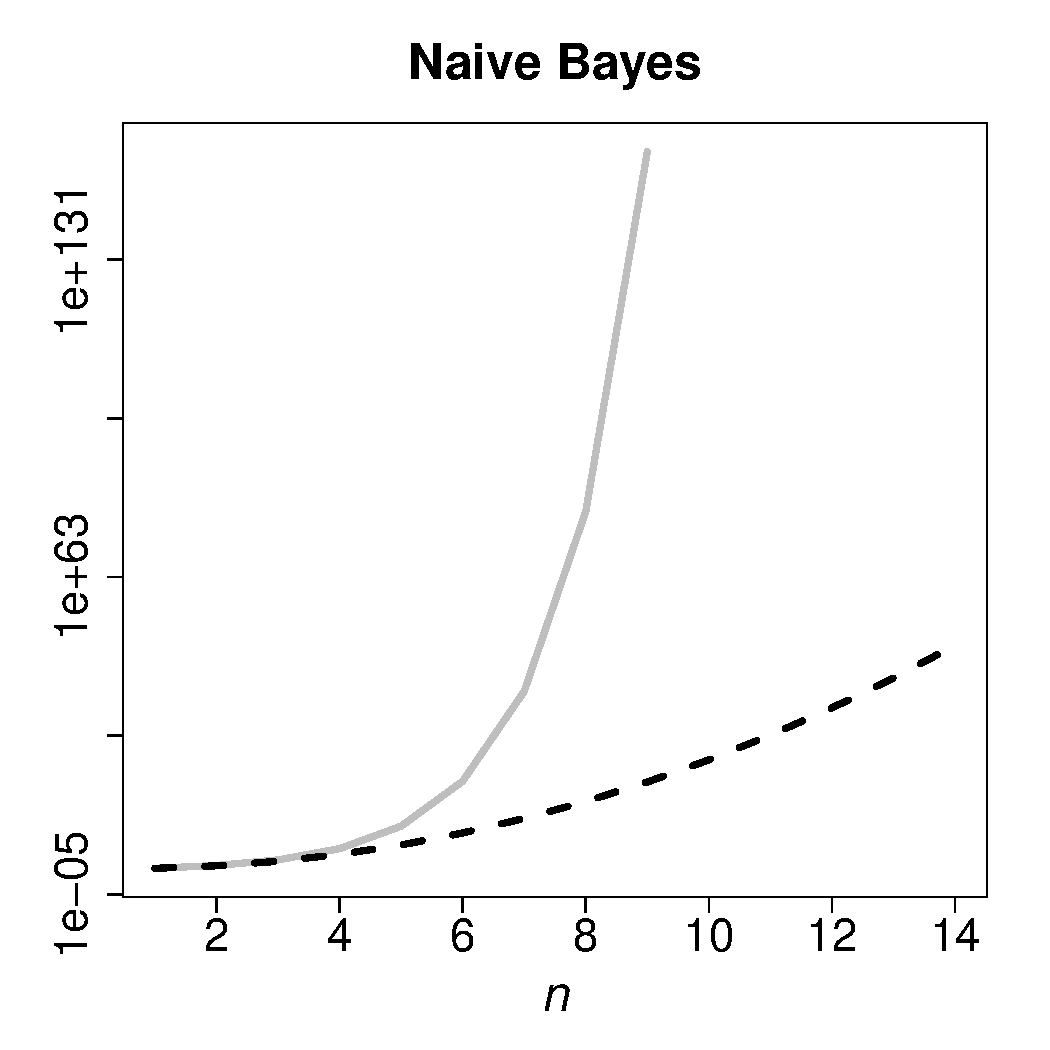
\includegraphics[scale=0.35]{NBvsTOTAL}
\caption{}
\label{fig:graph1}
\end{subfigure}
\centering
\begin{subfigure}{0.45\textwidth}
\centering
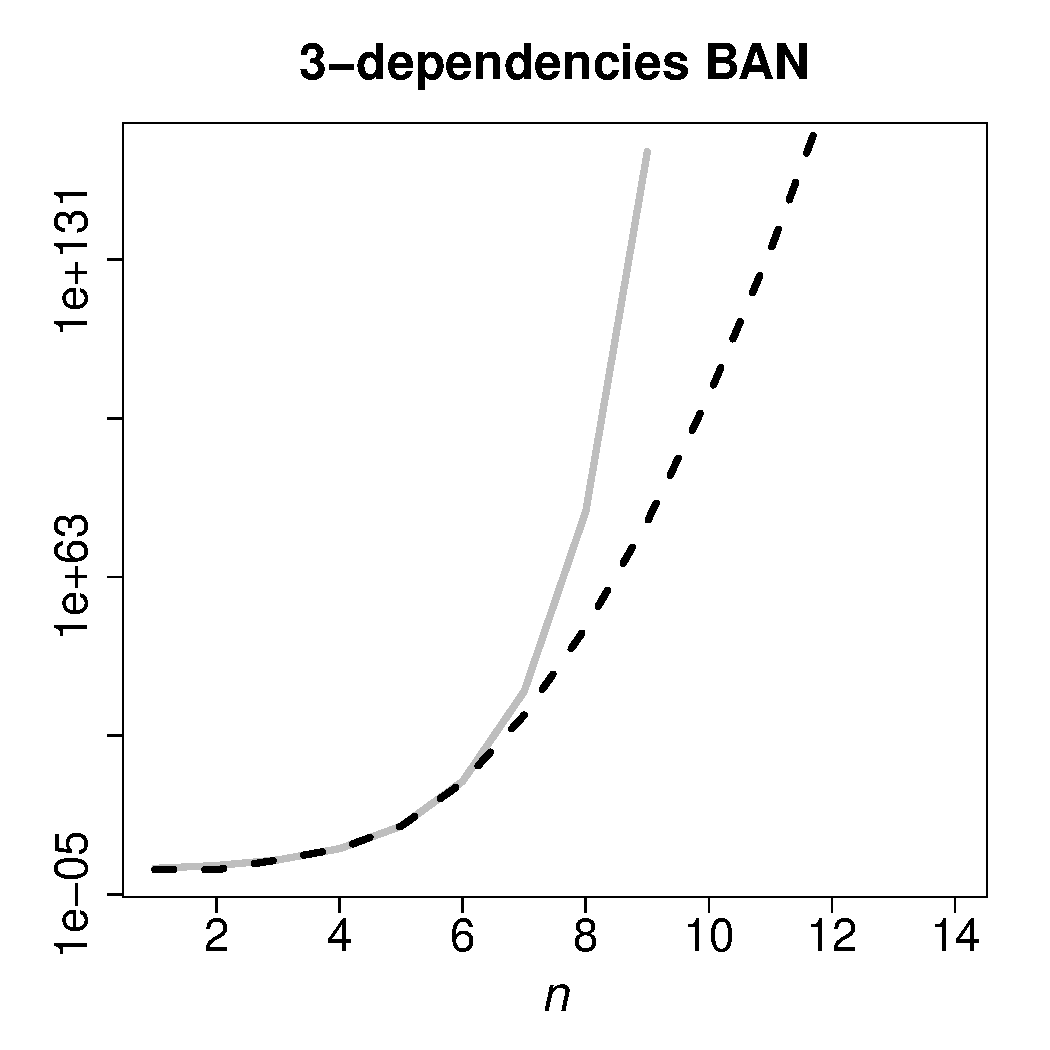
\includegraphics[scale=0.35]{BAN3vsTOTAL}
\caption{}
\label{fig:graph2}
\end{subfigure}
\caption{Total number of decision functions over $n$ binary predictors (solid gray) and the bounding $C(M,d)$ of Corollary \ref{cor:bounding} (dashed black) for NB classifiers (a) and for 3-dependence BAN classifiers (b)}
\label{fig:graph}
\end{figure}

\section{Conclusions}
\label{sec:conclusion}
In this chapter we have shown how to build polynomial threshold functions related to Bayesian network classifiers.
Our results reveal connections between the algebraic structure of the decision functions induced by BN classifiers and the topology of the structure of the predictor subgraph. 
In absence of $V$-structures in the predictor subgraph we have also proved that the specific polynomial representation fully characterized the type of Bayesian network classifier.
By representing classifiers by polynomial threshold functions, we can obtain bounds on the number of decision functions which can be induced by Bayesian network classifiers with a given structure.
The bounding does not hold in presence of $V$-structures in the predictor subgraph. Strong characterizations of induced decision functions cannot be proven due to the conditional independence of $V$-structure.
The polynomial representation of the discrimination functions of BAN classifiers implies the results of \cite{Roos2005} that connect Bayesian network classifiers and generalized logistic regression models.
%We observe that the $V$-structure independences are not reflected in the polynomial representation with linear relations among the coefficients. 
Moreover we observe that the obtained polynomial representation permits to easily prove the results of \citet{Ling03} for BAN classifiers without $V$-structures.

The bounds points to the fact, already conjectured by \citet{peot} for naive Bayes, that if we fix the maximum number of parents in a Bayesian network classifier, the type of classifier considered is not \textit{scalable}, in other words, more complex classifiers are expected to perform better when dealing with a large number of predictor variables. 

Moreover, the resulting bounds for the number of decision functions representable are strictly upper bounds since the subspaces generated by the different Bayesian networks considered are not in general position. What happens in the case of subspaces not in general position? Clearly we have to define some other property to characterize the \textit{position} of a subspace with respect to orthants in some given basis and try to count the number of such intersected orthants. With similar geometric results we will be able to precisely count the number of decision functions representable  by a given Bayesian network classifier, and we will be able to compute the gain in expressibility from simple to more complicated Bayesian network classifiers. 


\chapter{Decision Functions for Chain Classifiers Based on Bayesian Networks for Multi-Label Classification}

\label{chp:multilabel}

\section{Introduction}
We consider a multi-label classification problem \citep{zhang2013review,Tsoumakas07} over categorical predictors, that is, mapping every instance $\mathbf{x}=(x_1,\ldots,x_n)$ to a subset of $h$ labels:
\[ \bchi= {\nchi}_1\times\cdots\times{ \bchi}_n  \to  Y \textcolor{black}{\subseteq} \mathcal{Y}=\{ y_1,\ldots,y_{h}\}, \]
where ${\nchi}_{i} \subset \mathbb{R}$, $|{ \nchi}_i|=m_i<\infty$.
As usually the problem could be transformed into a multi-dimensional binary classification problem, that is, finding an $h$-valued decision function $\bm{\phi}$ that maps every instance of $n$ predictor variables $\mathbf{x}$ to a vector of $h$ binary values $\mathbf{c}=(c_1,\ldots,c_{h})\in \{-1,+1\}^{h}$:
$$
\begin{array}{ccccc}
\bm{\phi}:\quad &  \bchi={ \nchi}_{1}\times\cdots\times{ \nchi}_{n}  &\to&  \{-1,+1\}^{h} &\\ \\
  &\text{ } (x_1,\ldots,x_n) &\mapsto&  (c_1,\ldots,c_{h}),& 
 \end{array}
$$
where $c_i=+1$ ($-1$) means that the $i$-th label is present (absent) in the predicted label subset $Y$.
We consider the predictor variables $X_1,\ldots,X_n$ and the binary classes $C_i\in \{-1,+1\}$ as categorical random variables.
Real examples include classification of texts into different categories \citep{goncalves}, diagnosis of multiple diseases from common symptoms and identification of multiple biological gene functions \citep{Blockeel,Zhang2007}.

The easiest way to approach a multi-label classification problem is to divide it into a set of single-label classification problems (equivalent to binary classification problems).
Each binary problem is then solved independently and thus $h$ binary classifiers, one for each class variable $C_i$, are built. Each binary classifier is learned from predictor variables and $C_i$ data only. At the end the results are combined to form multi-label prediction. Known as \textit{binary relevance}, this method is easily implementable, has low computational complexity and is fully parallelizable. Therefore it is scalable to a large number of classes. However, it completely ignores dependencies among labels and generally does not represent the most likely set of labels. 

Chain classifiers \citep{reed2009,icml2010_037} relax the independence assumption by iteratively adding class dependencies in the binary relevance scheme. The $k$-th classifier in the chain predicts class $C_k$ from $X_1,\ldots,X_n,C_1,\ldots,C_{k-1}$. \cite{sucar2014} employed naive Bayes within chain classifiers. 

In this chapter, we study differences in the \textit{expressive power} of these two methods when Bayesian network (BN) classifiers \citep{bielza2014} are used. 
In particular, we extend the results of Chapter \ref{chp:decbound} to multi-label classifiers. Moreover, we suggest some theoretical reasons why the simple binary relevance method can perform poorly when relationships among labels exist, and we prove that chain classifiers provide more expressive models. 

%A broader chain classifiers class than in \cite{varandopgm} is considered and studied extensively and a bounding on the expressive power of those models is proved. Moreover we present novel illustrative examples both about the one-dimensional results and about multi-label ones.}

\subsection{Chapter Outline}
We describe the binary relevance method and compute its expressive power in Section \ref{sec:binary-relevance}. We analyze chain classifiers in Section \ref{sec:chain}. In Section \ref{sec:comparis} we compare the two methods, proving that actually chain classifiers are more expressive than binary relevance and  in Section \ref{sec:conclusions} we present our conclusions and some ideas for future research. 

\section{BAN Binary Relevance Classifiers}
\label{sec:binary-relevance}
We consider the binary relevance method built upon BAN classifiers as base models, that is, 
for every class variable $C_i$ we learn a BAN classifier with predictor subgraph $\mathcal{G}_i$. 
Thus we actually transform our multi-label problem into a number of single binary-class problems. The results of last chapter are then straightforwardly applied. 

From Lemma \ref{lem:BAN} it follows that if $\bm{\phi}=(\phi_1(\mathbf{x}),\phi_2(\mathbf{x}),\ldots,\phi_{h}(\mathbf{x}))$ is the $h$-valued decision function induced by the $h$ BAN classifiers, then there exist $$p_1(\mathbf{x})\in \mathcal{P}_{\mathcal{G}_1} ,\ldots,p_{h}(\mathbf{x}) \in \mathcal{P}_{\mathcal{G}_h},$$
such that $\phi_k(\mathbf{x})=sign(p_k(\mathbf{x}))$ for every $k \in \{1,\ldots,h\}$. We have then that the multi-valued decision function has a polynomial representation as,
$$ {\bm{\phi} }(\mathbf{x})=\big( sign(p_1(\mathbf{x})),\ldots,sign(p_h(\mathbf{x})) \big). $$

When we also assume that the predictor subgraphs $\mathcal{G}_1,\ldots,\mathcal{G}_h$ contain no $V$-structures, we have that, for every single binary-class problem, Theorem \ref{teo:BAN} applies.
Thus, in Lemma \ref{lem:brbound}, we bound the number of multi-valued decision functions representable by the BAN binary relevance method, when the predictor subgraphs $\{\mathcal{G}_k\}_{k=1}^h$ do not contain V-structures.

\begin{lemma}
\label{lem:brbound}
Consider $h$ BAN classifiers to predict $h$ binary classes. Suppose that the predictor subgraphs are  $\mathcal{G}_1,\ldots,\mathcal{G}_h$ respectively and they contain no V-structures. We have that $N\left(\mathcal{G}_1,\ldots,\mathcal{G}_h\right)$, the number of $h$-valued decision functions representable by the BAN binary relevance method, satisfies
\[ N\left(\mathcal{G}_1,\ldots,\mathcal{G}_h\right) \leq \prod_{k=1}^{h} C(M,d_k), \]
where $C(M,d)=2\sum_{k=0}^{d-1}{M-1 \choose k }$, $d_k=\sum_{i=1}^n \left( (m_i-1)\prod_{s \in {pa}_k(i)} m_s \right)+1$, ${pa}_k(i)$ is the set of $X_i$ parents in $\mathcal{G}_k$ and $M=\prod_{i=1}^n m_i$.
\end{lemma}
\begin{proof}
The proof  is a straightforward application of Corollary \ref{cor:bounding}. 
\end{proof}

\begin{remark}
We consider now, for visualization purposes, a simpler version of the above models. In particular when the predictors subgraphs are all the same, that is, $\mathcal{G}_j=\mathcal{G}$.  
The total number of $h$-valued decision functions over $n$ categorical predictors is $2^{h \prod m_i}=2^{h M}$. Then the fraction of $h$-valued decision functions representable by the BAN binary relevance method is bounded by
\[ \frac{N\left(\mathcal{G}_1,\ldots,\mathcal{G}_h\right)}{2^{h M}}\leq \left( \frac{C(M,d)}{2^M} \right)^{h} .\]
Thus, we have that if we fix the structure of the predictor subgraph, and it does not contain V-structures, the number of representable multi-valued decision functions becomes vanishingly small as the number of predictors increase. Moreover, using the binary relevance method, the \textit{speed} at which the ratio between representable multi-valued decision functions and the total number of multi-valued decision functions drops to zero, is exponential in $h$, the number of classes.
\end{remark}

\begin{example}
\label{exp:ml1}
\begin{figure}
\centering
\begin{tikzpicture}[->,>=stealth',shorten >=1pt,auto,node distance=3cm,
  thick,main node/.style={circle,fill=white!20,draw,font=\sffamily\Large\bfseries},minimum width=1.5cm]
  
  \node[main node] (1) {$C_1$};
  \node[main node] (3) [below left of=1] {$X_1$};
  \node[main node] (2) [below right of=1] {$X_2$};
  \node (7) [right of=1] {};
  \node[main node] (6) [right of=7] {$C_2$};
  \node[main node] (4) [below left of=6] {$X_1$};
  \node[main node] (5) [below right of=6] {$X_2$}; 
  
  \path[every node/.style={font=\sffamily\small}]
    (1) edge node [left] {}  (2)
        edge node[left] {} (3);
        
  \path[every node/.style={font=\sffamily\small}]
    (6) edge node [left] {}  (4)
        edge node[left] {} (5);      

\end{tikzpicture}  
\caption{Two NB classifiers in Example \ref{exp:ml1}}
\label{fig:NBbrm}
\end{figure}
We consider two binary classes $C_1,C_2$ and two predictor variables $X_1 \in \{0,1\}$ and $X_2 \in \{2,3,4\}$.
Using the binary relevance method we build two independent NB classifiers, see Figure \ref{fig:NBbrm}.
Next, we list the conditional probability tables for both classifiers (Tables \ref{tab:condprob1ml} and \ref{tab:condprob2}). \textcolor{black}{Moreover, we consider uniform prior probabilities for both classes $C_1$ and $C_2$.}


\begin{table}
\caption{Conditional probability tables in Example \ref{exp:ml1} for the NB of $C_1$}
\centering
\label{tab:condprob1ml}
\begin{subtable}{0.4\textwidth}
\textcolor{black}{
\begin{tabular}{cccc}
\toprule
\multicolumn{2}{c}{$\Pp(X_1|C_1)$}  &  \multicolumn{2}{c}{$X_1$}\\
&  &  0    &   1 \\
\cmidrule{3-4}
\multirow{2}{0.5cm}{$C_1$} 
 & $-1$ & 0.25 & 0.75 \\
 & $+1$ & 0.5 & 0.5 \\
 \bottomrule
\end{tabular}}
\end{subtable}
\begin{subtable}{0.4\textwidth}
\textcolor{black}{\begin{tabular}{ccccc}
\toprule
\multicolumn{2}{c}{$\Pp(X_2|C_1)$}  &  \multicolumn{3}{c}{$X_2$}\\
&  &  2    &   3  & 4 \\
\cmidrule{3-5}
\multirow{2}{0.5cm}{$C_1$} 
 & $-1$ & 0.1 & 0.7 & 0.2 \\
 & $+1$ & 0.3 & 0.5 & 0.2 \\
 \bottomrule
\end{tabular}}
\end{subtable}
\end{table}


\begin{table}
 \caption{Conditional probability tables in Example \ref{exp:ml1} for the NB of $C_2$}
\label{tab:condprob2}
\centering
\begin{subtable}{0.4\textwidth}
\textcolor{black}{
\begin{tabular}{cccc}
\toprule
\multicolumn{2}{c}{$\Pp(X_1|C_2)$}  &  \multicolumn{2}{c}{$X_1$}\\
&  &  0    &   1 \\
\cmidrule{3-4}
\multirow{2}{0.5cm}{$C_2$} 
 & $-1$ & 0.4 & 0.6 \\
 & $+1$ & 0.7 & 0.3 \\
 \bottomrule
\end{tabular}}
\end{subtable}
\begin{subtable}{0.4\textwidth}
\textcolor{black}{\begin{tabular}{ccccc}
\toprule
\multicolumn{2}{c}{$\Pp(X_2|C_2)$}  &  \multicolumn{3}{c}{$X_2$}\\
&  &  2    &   3  & 4 \\
\cmidrule{3-5}
\multirow{2}{0.5cm}{$C_2$} 
 & $-1$ & 0.6 & 0.2 & 0.2 \\
 & $+1$ & 0.1 & 0.1 & 0.8 \\
 \bottomrule
\end{tabular}}
\end{subtable}


\end{table}
From the representation of Theorem \ref{teo:BAN} we have that there exist two polynomials $p_1,p_2$ that sign-represent the decision functions induced by the two NB classifiers
\begin{align*}
p_1(x_1,x_2) =&\log\left(\frac{0.5}{0.25}\right) \frac{x_1-1}{-1} + \log\left( \frac{0.5}{0.75} \right) \frac{x_1}{1}  \\ 
          +& \log\left(\frac{0.3}{0.1}\right) \frac{(x_2-3)(x_2-4)}{2} + \log\left(\frac{0.5}{0.7}\right) \frac{(x_2-2)(x_2-4)}{-1} \\
   +& \log\left(\frac{0.2}{0.2}\right) \frac{(x_2-2)(x_2-3)}{2}
\end{align*} 
and
\begin{align*}
p_2(x_1,x_2)=&\log\left(\frac{0.7}{0.4}\right) \frac{x_1-1}{-1} + \log\left( \frac{0.3}{0.6} \right) \frac{x_1}{1}  \\ 
           +& \log\left(\frac{0.1}{0.6}\right) \frac{(x_2-3)(x_2-4)}{2} + \log\left(\frac{0.1}{0.2}\right) \frac{(x_2-2)(x_2-4)}{-1} \\ 
           + &\log\left(\frac{0.8}{0.2}\right) \frac{(x_2-2)(x_2-3)}{2}.
\end{align*} 
We have that
\[ \bm{\phi}(\mathbf{x})=\bigg( sign\big(p_1(\mathbf{x}) \big), sign\big( p_2(\mathbf{x}) \big) \bigg) \]
is the bi-valued decision function that predicts $C_1,C_2$ from $X_1,X_2$.
Figure \ref{fig:decbound} shows the decision boundaries of the two classifiers (black for $C_1$ and gray for $C_2$). We observe that the predictor space ${\bchi}=\{0,1\}\times\{2,3,4\}$ is partitioned into four subsets corresponding to the four different predictions of the two binary classes. The value of the respective predicted class changes when one of the decision boundaries is crossed. 
\begin{figure}[h!]
\centering
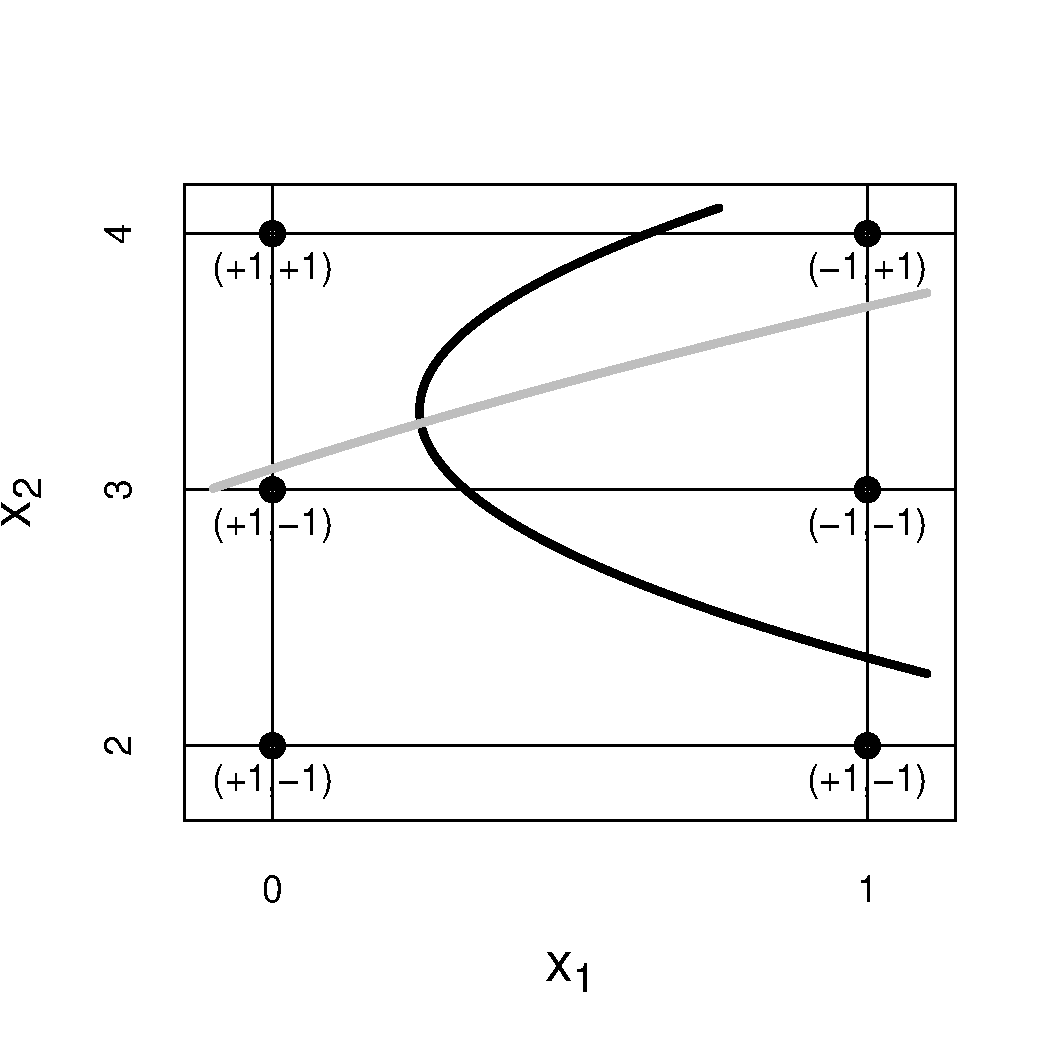
\includegraphics[scale=0.5]{ExampleBR}
\caption{Decision boundaries for the two NB classifiers in Example \ref{exp:ml1}, black for $C_1$ and gray for $C_2$. The value of the predicted classes is reported}
\label{fig:decbound}
\end{figure}
\end{example}
\section{BAN Chain Classifiers}
\label{sec:chain}
The easiest way to relax the strong independence assumption of the binary relevance method is to gradually add the predicted classes to the predictors. Specifically, suppose that we have to predict $h$ binary classes $C_1,\ldots,C_{h}$ from $n$ predictor variables $X_1,\ldots,X_n$.
We consider $h$ BAN classifiers such that the $k$-th BAN classifier predicts $C_k$ from the variables $$X_1,\ldots,X_n,C_1,\ldots,C_{k-1}.$$
{In the predicting phase we will then use the predictor values and the previous predicted classes values $\hat{c}_1,\ldots,\hat{c}_{k-1}$ to predict class $C_k$.}
From Lemma \ref{lem:BAN} we have that there exist $h$ polynomials $p_1,\ldots,p_{h}$ 
\[ p_k(\mathbf{x},\hat{c}_1,\ldots,\hat{c}_{k-1}): \mathbb{R}^{n+k-1} \to \mathbb{R} \]
\[ p_k \in \mathcal{F}_{\mathcal{G}_k}, \]
such that, if ${\bm{\phi}}=(\phi_1,\ldots,\phi_h)$ is the multi-valued decision function associated with a chain classifier we have that, 
\begin{equation}
\label{eq:chainpolynomial} \phi_k(\mathbf{x})=sign(p_k(\mathbf{x},\phi_1(\mathbf{x}),\ldots,\phi_{k-1}(\mathbf{x})))\end{equation}
where $\mathcal{G}_k$ is the predictor subgraph related to the $k$-th BAN classifier over  $X_1,\ldots,X_n$ and $C_1,\ldots,C_{k-1}$.

From now on we will focus on a particular and simpler form of BAN chain classifier, where the previous predicted classes are present in a naive way in the predictor subgraph. That is, $C_1,\ldots,C_{k-1}$ are not connected among them neither with other predictors in the subgraph $\mathcal{G}_k$.
We refer to this kind of chain classifier as \textit{naive BAN chain classifier}, see an example in Figure \ref{fig:chainnaive}.
As we will see those naive models have a more simpler representation of multi-valued decision functions and permit a deeper analysis. \textcolor{black}{We observe that more complex chain models could be addressed in a similar way, using the interpolating polynomials to represent the decision functions of the already predicted classes. In more complex models, however, the analysis of the decision function is more difficult and not all the following results can be extended directly. }
 
\begin{figure}[h!]
\centering
\begin{tikzpicture}[->,>=stealth',shorten >=1pt,auto,node distance=2cm,
  thick,main node/.style={circle,fill=white!20,draw},minimum width=0.1cm]
  
  \node[main node] (1) {$C_1$};
  \node[main node] (2) [below left of=1] {$X_1$};
  \node[main node] (3) [below right of=1] {$X_2$};
  \node[main node] (4) [below of=1] {$X_3$};

  \node (5) [right of=1] {};

  \node[main node] (6) [right of=5] {$C_2$};
  \node[main node] (7) [below of=6] {$X_1$};
  \node[main node] (8) [below right of=6] {$X_2$}; 
  \node[main node] (9) [below of=8] {$X_3$};
  \node[main node] (10) [below left of=6] {$C_1$};
  
  \node[main node] (11) [right of=6] {$C_2$};

  \node[main node] (12) [right of=11] {$C_3$};
  \node[main node] (13) [below of=12] {$X_1$};
  \node[main node] (14) [below right of=12] {$X_2$}; 
  \node[main node] (15) [below of=14] {$X_3$};
  \node[main node] (16) [below left of=12] {$C_1$};
  %\node[main node] (17) [right of=6] {$C_2$};
    
  \path[every node/.style={font=\sffamily\small}]
    (1) edge node [left] {}  (2)
    edge node [left] {}  (4)
        edge node[left] {} (3);
        
  \path[every node/.style={font=\sffamily\small}]
    (6) edge node [left] {}  (7)
        edge node [left] {}  (8)
        edge node [left] {}  (9)
        edge node[left] {} (10)
    (7) edge node [left] {} (8)
    (9) edge node [left] {} (8);    
              
        
  \path[every node/.style={font=\sffamily\small}]
    (12) edge node [left] {}  (13)
        edge node [left] {}  (14)
        %edge node [left] {}  (15)
        edge node [left] {}  (16)
        edge node[left] {} (11)
        edge node [left] {} (15)
     (14) edge node [left] {} (13)
          edge node [left] {} (15);

\end{tikzpicture}  
\caption{Example of naive BAN chain classifier with three classes and three predictor variables }
\label{fig:chainnaive}
\end{figure}
For a naive BAN chain classifier for $C_1,\ldots,C_h$, over $X_1,\ldots,X_n$ we denote by $\mathcal{H}_k$ the subgraph of the $k$-th BAN restricted to the original predictors $X_1,\ldots,X_n$. 

\textcolor{black}{Since classes $C_j$ are binary, expanding Equation (\ref{eq:chainpolynomial}) we obtain the following sign-representation of the $k$-th decision function in a naive BAN chain classifier:
\begin{align*}
\phi_k(\mathbf{x})=sign&( p_k(\mathbf{x},\phi_{1}(\mathbf{x}),\ldots,\phi_{{k-1}}(\mathbf{x}))\\
=sign & \left(\sum_{i=1}^{n}  \sum_{j=1}^{m_i}\ell_{j}^{{ \nchi}_i}(x_i) \sum_{\mathbf{k}\in \mathbb{M}_i} \beta_{i}(j|\mathbf{k})\prod_{s\in  {pa}(i)} \ell_{k_s}^{{ \nchi}_{s}}(x_{s})\right.  \\
 &+  \left. \sum_{j=1}^{k-1}\left[ \beta_j(-1)\ell_{-1}^{\{-1,+1\}}(\hat{c}_j)+\beta_j(+1)\ell_{+1}^{\{-1,+1\}}(\hat{c}_j)\right]\right)\\
=sign&\left(\hat{q}_k(\mathbf{x})+\sum_{j=1}^{k-1} \left[ \beta_j(-1)\ell_{-1}^{\{-1,+1\}}(\hat{c}_j)+\beta_j(+1)\ell_{+1}^{\{-1,+1\}}(\hat{c}_j)\right] \right),
\end{align*}
where $\hat{q}_k\in \mathcal{P}_{\mathcal{H}_k}$, $\hat{c}_j=\phi_{j}(\mathbf{x})$ is the predicted value of the previous classifier expressed by the interpolating polynomial as a function of $\mathbf{x}$, $\ell_{-1}^{\{-1,+1\}}(c)=\frac{c-1}{-2}$ and $\ell_{+1}^{\{-1,+1\}}(c)=\frac{c+1}{2}$ are the Lagrange basis polynomials over $\{-1,+1\}$ and $\beta_j(c)=\log\left(\frac{\Pp(C_j=c|C_k=+1)}{\Pp(C_j=c|C_k=-1)}\right)$.
Rearranging the terms in the sum we obtain that the following function sign-represents $\phi_k$,}
\begin{equation}
q_k(\mathbf{x})=\hat{q}_k(\mathbf{x})+\sum_{j=1}^{k-1}\left( a_j \phi_{j}(\mathbf{x})+b_j\right),
 \label{eq:chainpoly} 
\end{equation}
where $\phi_j$ are the decision functions of the previous predicted class in the chain, $\hat{q}_k$ is the polynomial related to the subgraph $\mathcal{H}_k$ as in Theorem \ref{teo:BAN} and
\begin{align} a_j=& \frac{1}{2}\log\left( \frac{ \Pp(C_j=+1|C_k=+1)\Pp(C_j=-1|C_k=-1)}{\Pp(C_j=+1|C_k=-1)\Pp(C_j=-1|C_k=+1)}\right)\label{eq:coeff1} \\
 b_j=& \frac{1}{2}\log\left( \frac{ \Pp(C_j=+1|C_k=+1)\Pp(C_j=-1|C_k=+1)}{\Pp(C_j=+1|C_k=-1)\Pp(C_j=-1|C_k=-1)}\right)\label{eq:coeff2}  
 \end{align}


Observe that we can omit constants $b_j$ in Equation (\ref{eq:chainpoly}) if analysing the expressive power. In fact constants could be included in the polynomial $\hat{q}_k$ using elementary properties of Lagrange basis polynomials, see Chapter \ref{chp:decbound}. 
The following lemma describes the set of decision functions induced by the $k$-th step of the naive BAN chain classifier.

\begin{lemma}
Consider a multi-label classification problem over predictors $X_1,$ $\ldots,X_n$ and a naive BAN chain classifier with predictor subgraphs $\mathcal{H}_1,\ldots,\mathcal{H}_h$ for classes ordered as $C_1,$ $\ldots$, $C_h$. Assume that the predictor subgraphs do not contain $V$-structures.
For every $k\in \{2,\ldots,h\}$ we have that, if $\phi_1,\ldots,\phi_{k-1}$ are the decision functions for $C_1,\ldots,C_{k-1}$ respectively, then the following set of polynomials sign-represent every decision function for class $C_k$,
$$ \mathcal{F}_{\mathcal{H}_k} + <\phi_{1},\ldots,\phi_{{k-1}}> ,$$
where $<\ldots >$ denotes the span of the included vectors and the sum is intended as the sum of two vectorial spaces, that is, the vectorial space which includes all the possible sum of elements of the two  spaces, $\mathcal{F}_{\mathcal{H}_k}$ and  $<\phi_{1},\dots,\phi_{{k-1}}>$.
\end{lemma}
\begin{proof}
The proof of the result is just an application of Theorem \ref{teo:BAN} and Equation (\ref{eq:chainpoly}).
\end{proof}

We have furthermore, that the set $sign\left(\mathcal{F}_{\mathcal{H}_k}+<\phi_{1},\ldots,\phi_{{k-1}}>\right)$ is equal to the set of decision functions representable by the $k$-th BAN classifier of the naive BAN chain classifier if the graphs $\mathcal{H}_k$ do not contain $V$-structures.
\textcolor{black}{Intuitively, from an expressive-power point of view, we have the addition of the previous predicted classes in the $k$-th step of a naive BAN chain classifier being the equivalent to the \textit{enrichment} of the space of functions $\mathcal{F}_{\mathcal{H}_k}$, related to the original predictors, by a subspace generated by the previously induced decision functions.
To analyze if and how the enlarged space is indeed a bigger space, in other words, that it has a higher dimension, we have to understand when a decision function $\phi \in \mathcal{C}$ does not belong to a space of the type $\mathcal{F}_{\mathcal{G}}$ for some graph $\mathcal{G}$. Thus, in this case, adding $<\phi>$ to $\mathcal{F}_{\mathcal{G}}$ will actually increase the dimension.}

First of all we define the set of relevant variables for a given decision function.
\begin{definition}
Given a decision function $$\phi(x_1,\ldots,x_n): {\bchi}=\nchi_1\times\cdots\times\nchi_n \to \mathbb{R}$$ we say that a variable $X_i$ is irrelevant for $\phi$ if 
$$ \phi(x_1,\ldots,x_n)=g(\mathbf{x}_{-i})=\psi(x_1,\ldots,x_{i-1},x_{i+1},\ldots,x_n), \quad \forall (x_1,\ldots,x_n) \in {\bchi}.$$
A variable is said to be relevant for $\phi$ if it is not irrelevant, and we indicate with $\mathcal{V}(\phi)$ the set of relevant variables for $\phi$.
\end{definition}
\textcolor{black}{As we will see relevant variables are important in order to determine if a given decision function belongs or not to some space $\mathcal{F}_{\mathcal{G}}$. In real applications the task of finding relevant variables of a decision function is computationally expensive and moreover in reality we usually know just an estimation of a decision function or its value on a set of random points. The presented analysis is thus intended as a theoretical analysis.}
\textcolor{black}{\begin{example}
We show some examples of decision functions and their respective set of relevant variables.
\begin{enumerate}
\item If $\phi_1$ is a decision function over $\{0,1,2\}\times \{-3,-2\}$, such that
$$ \phi_1(x_1,x_2)=\begin{cases}
    -1 & \text{if } (x_1,x_2)=(0,-3) \text{ or } (0,-2) \\
    +1 & \text{otherwise}.
\end{cases}$$
Then obviously $\phi_1(x_1,x_2)=g(x_1)$, where $g(x_1)=-1$ if $x_1=0$ and $+1$ otherwise. Thus $X_2$ is irrelevant for $\phi_1$ and $\mathcal{V}(\phi_1)=\{X_1\}$.
\item If $\phi_2$ is the xor-function over $\{0,1\}\times\{0,1\}$, defined as follows
$$ \phi_2(x_1,x_2)=\begin{cases}
    -1 & \text{if } (x_1,x_2)=(0,0) \text{ or } (1,1) \\
    +1 & \text{if } (x_1,x_2)=(0,1) \text{ or } (1,0).
\end{cases}$$
Then $\mathcal{V}(\phi_2)=\{X_1,X_2\}$ and $\phi_2$ does not have irrelevant variables.
\item If $\phi_3$ is the function over $\{0,1\}\times\{0,1\}$ such that,
$$ f_3(x_1,x_2)=\begin{cases}
    -1 & \text{if } (x_1,x_2)=(0,0)  \\
    +1 & \text{otherwise} .
\end{cases}$$
Then also in this case $\mathcal{V}(\phi_3)=\{X_1,X_2\}$.
\end{enumerate}
\label{exp:relevant}
\end{example}}
\textcolor{black}{We can now state the following result about the set of relevant variables of  decision functions.}
\begin{lemma}
\label{lem:relevant}
Consider a graph $\mathcal{G}$ without $V$-structures and the space of functions $\mathcal{F}_{\mathcal{G}}$ defined in Equation (\ref{eq:defspace3}). For every decision function $\phi$ we have that,
$$ \phi \in \mathcal{F}_{\mathcal{G}} \Leftrightarrow \mathcal{V}(\phi) \text{ are completely connected in } \mathcal{G}.$$
\end{lemma}
\begin{proof}
If the relevant variables for $\phi$ are completely connected in the graph $\mathcal{G}$, then we have that the polynomials in $\mathcal{F}_{\mathcal{G}}$ could interpolate over $\bchi$ any function of variables in $\mathcal{V}(\phi)$ only. In particular, there exists a polynomial $p(\mathbf{x})\in\mathcal{\phi}_{\mathcal{G}}$ such that $\phi(\mathbf{x})=p(\mathbf{x})$, $\forall \mathbf{x}\in{\bchi}$ and thus $\phi \in \mathcal{F}_{\mathcal{G}}$.

To prove the other implication we observe that if two variables $X_i$ and $X_j$ are not directly connected in the graph $\mathcal{G}$, each polynomial $p(\mathbf{x})\in \mathcal{F}_{\mathcal{G}}$ could be split into the sum of two polynomials,
\begin{equation} p(\mathbf{x})=p_1(\mathbf{x}_{-\{i,j\}},x_i)+p_2(\mathbf{x}_{-\{i,j\}},x_j).
\label{eq:polsplit}
 \end{equation} 
\textcolor{black}{To prove the above equality we just observe that each polynomial $p$ in $\mathcal{F}_{\mathcal{G}}$ has the following expression
$$ p(\mathbf{x})=\sum_{i=1}^{n}\sum_{j=1}^{m_i} \ell_{j}^{\nchi_i}(x_i)\sum_{\mathbf{k} \in \mathbb{M}_i}\beta_i(j|\mathbf{k})\prod_{s\in{\bf pa}(i)}\ell_{k_s}^{\nchi_s}(x_s).$$
Thus two variables appear in the same product of different Lagrange polynomial bases if and only if they are directly connected, that is, if and only if one variable belongs to the parents of the other.
It is clear now that the sum in Equation (\ref{eq:polsplit}) is therefore valid.  
 }
So we have only to prove that a decision function $\phi \in \mathcal{C}$ with two relevant variables $X_1\in\nchi_1,X_2\in\nchi_2$ could not be equal, over $\nchi_1\times\nchi_2$, to the sum of two functions $p_1(x_1)$ and $p_2(x_2)$.
Since $X_1$ and $X_2$ are relevant variables, there exist $s,s'\in\nchi_1$ and $t,t'\in\nchi_2$ such that,
$$ \phi(s,t)=- \phi(s,t') \quad \text{and} \quad \phi(s,t)=-\phi(s',t) $$
Suppose $\phi(x_1,x_2)=p_1(x_1)+p_2(x_2)$, then we have,
\begin{align*} \phi(s',t')=& p_1(s')+p_2(t') \\
=&p_1(s')+p_2(t)+p_1(s)+p_2(t')-p_1(s)-p_2(t) \\
=&\phi(s',t)+\phi(s,t')-\phi(s,t)=-3\phi(s,t).  
\end{align*}
And we get $|\phi(s',t')|\neq 1$ which is absurd given that $\phi$ is a decision function ($|\phi(\bx)| = 1$).
\end{proof}

\textcolor{black}{
We return to points 2 and 3 of Example \ref{exp:relevant}. In both cases functions $\phi_2$ and $\phi_3$ do not have irrelevant variables. Thus from Lemma \ref{lem:relevant} we have that $\phi_{2},\phi_{3} \notin \mathcal{F}_{NB}$. But $\phi_2 \notin sign(\mathcal{F}_{NB})$ (see the results of \cite{Ling03}) while $\phi_3 \in sign(\mathcal{F}_{NB})$ (see proof of Theorem \ref{teo:BRvsCH}).
}

\textcolor{black}{Thanks to Lemma \ref{lem:relevant}, we have the following result.}
\begin{lemma}
Consider a multi-label classification problem over \textcolor{black}{categorical} predictors $X_1,\ldots,X_n$, for \textcolor{black}{binary} classes ordered as $C_1,\ldots,C_h$. Given a sequence of predictor subgraphs $\mathcal{H}_1,\ldots,\mathcal{H}_h$ without $V$-structures, \textcolor{black}{let us} consider ${\phi}=(\phi_1,\ldots,\phi_h)$ the  $h$-valued decision functions of the corresponding naive BAN chain classifier.
\textcolor{black}{Then,} for every $1\leq k\leq h$, we have that
$$ \left| sign\left( \mathcal{P}_{\mathcal{H}_k} + <\phi_{1},\ldots,\phi_{{k-1}}>\right)\right|\leq C(M,d_k+s)\leq C(M,d_k+k-1) , $$
where $M=|{\bf \nchi}|=\prod_{i=1}^n m_i$, $d_k=\dim(\mathcal{P}_{\mathcal{H}_k})$, and $s$ is equal to the number of functions among $\phi_1,\ldots,\phi_{k-1}$ such that their relevant variables are not completely connected in $\mathcal{H}_k$.
\label{lem:boundingchain}
\end{lemma}
\begin{proof}
Suppose, $\phi_{i_1},\ldots,\phi_{i_s}$ are the decision functions among $\phi_1,\ldots,\phi_{k-1}$ such that their relevant variables are not completely connected in $\mathcal{H}_k$. From Lemma \ref{lem:relevant} we have that,
$$ \phi_{{i_1}},\ldots,\phi_{{i_s}} \notin \mathcal{P}_{\mathcal{H}_k},$$
\textcolor{black}{and that 
$$\phi_{{i}} \in \mathcal{P}_{\mathcal{H}_k} \text{ for every } i \in \{1,\ldots,k-1\}\setminus\{i_1,\ldots,i_s\},  $$
Thus we have 
$$\mathcal{P}_{\mathcal{H}_k}+<\phi_{1},\ldots,\phi_{{k-1}}>=\mathcal{P}_{\mathcal{H}_k}+<\phi_{{i_1}},\ldots,\phi_{{i_s}}>,$$
and so 
$$ \dim\left(\mathcal{P}_{\mathcal{H}_k}+<\phi_{1},\ldots,\phi_{{k-1}}>\right)\leq d_k+s \leq d_k+k-1.$$}
Analogously to Corollary \ref{cor:bounding} we have the corresponding bounding.
\end{proof} 

\begin{remark}
We observe that changing the order of classes in which the chain classifier is built implies a change in the expressive power of the resulting multi-label classifier. If the chain classifier is built with the class ordering $C_1,\ldots,C_{h}$,  we have that the $k$-th classifier for $C_{k}$ is \textit{more expressive} than all the previous classifiers in the chain.
In fact, from Equation (\ref{eq:chainpoly}), we have that if $\phi$  is a decision function representable by the $j$-th  step of the chain classifier, then $\phi$ is representable by every successive steps of the chain classifier.
\end{remark}

\begin{example}
\label{exp:ml2}
We use a NB chain classifier over the prediction problems of Example \ref{exp:ml1}. The NB classifier for predicting class $C_1$ is the same as in Example \ref{exp:ml1} (see Figure \ref{fig:NBbrm} left and Table \ref{tab:condprob1ml}). The predictors of the NB classifier for predicting $C_2$ now include $C_1$. We consider the same conditional probability tables as in Example \ref{exp:ml1} (Tables \ref{tab:condprob1ml} and \ref{tab:condprob2}). Moreover we have to specify the conditional probabilities of $C_1$ given $C_2$ in the NB that predicts $C_2$. We set
\[ \Pp(C_1=+1|C_2=+1)=0.3 \text{ and } \Pp(C_1=-1|C_2=+1)=0.7,  \]
\[ \Pp(C_1=+1|C_2=-1)=0.9 \text{ and } \Pp(C_1=-1|C_2=-1)=0.1.  \]
And, thus, coefficients $a_1$ and $b_1$ as defined in Equations (\ref{eq:coeff1}) and (\ref{eq:coeff2}) are given by
\[ a_1=\frac{1}{2}\log \left( \frac{0.3 \times 0.1}{0.9\times0.7} \right) \text{ and} \quad
 b_1=\frac{1}{2}\log \left( \frac{0.3\times0.7}{0.9\times0.1} \right).\]
We have that the decision function to predict $C_2$ is sign-represented by
\[ {q_2(x_1,x_2)=p_2(x_1,x_2) + a_1 \phi_{1}(x_1,x_2)+b_1 }\]
{where $\phi_1(x_1,x_2)=sign(p_1(x_1,x_2))$ and $p_2$ are defined in Example \ref{exp:ml1}.
The decision boundaries of the two classes are shown in Figure \ref{fig:NBchain1}.} We observe that the two boundaries are no longer independent; the decision boundary for the second class $C_2$ (dashed gray line) depends on the decision boundary of the first class $C_1$.
\begin{figure}[h!]
\centering
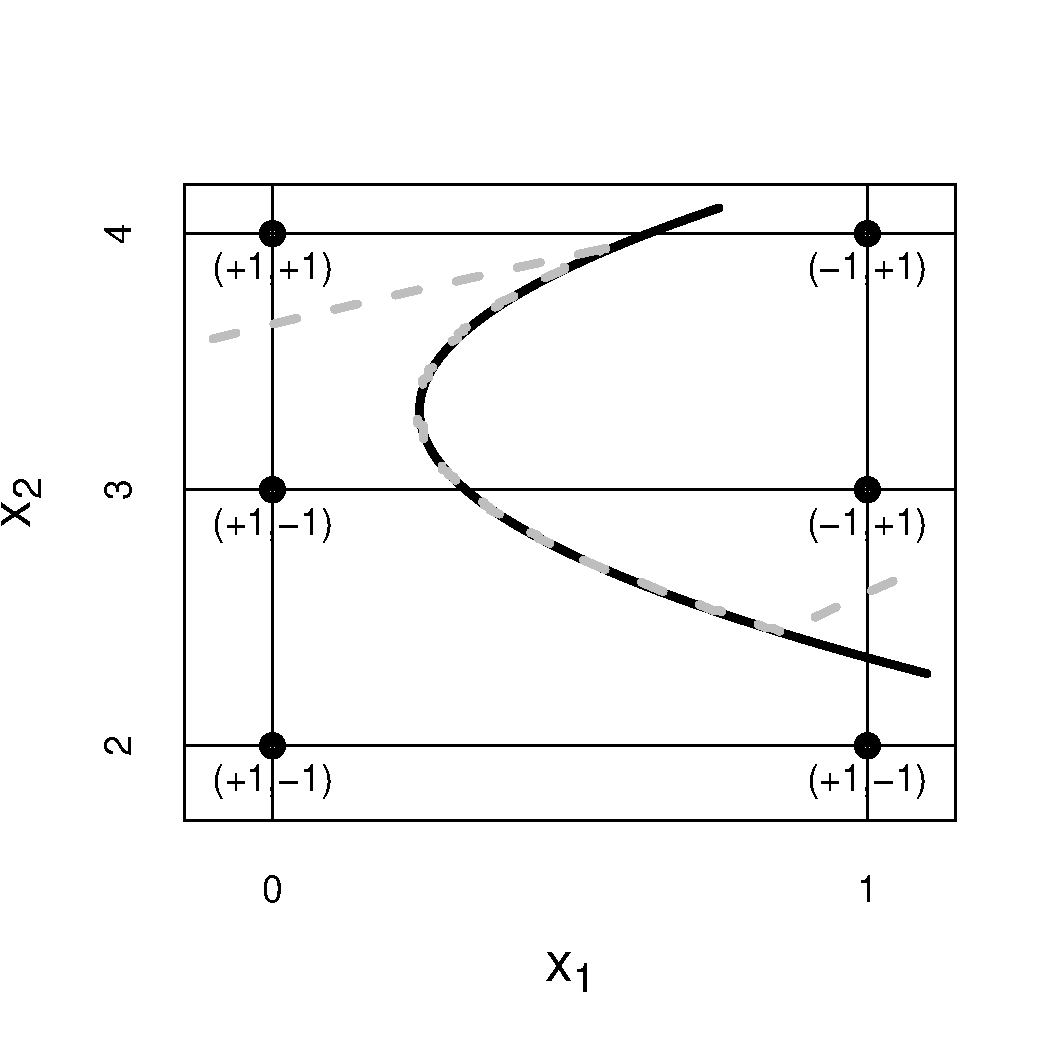
\includegraphics[scale=0.5]{ExampleChain}
\caption{Decision boundaries for the chain NB classifier in Example \ref{exp:ml2}. The value of the predicted classes is reported}
\label{fig:NBchain1}
\end{figure}
\end{example}


\textcolor{black}{
\subsection{Extensions to Classifier Trellises}
Classifier trellises (CT) are a novel paradigm to multi-label classification problems, recently introduced by \cite{Read2015}. Basically CT works as chain classifiers, but instead of adding as predictors all the previous predicted classes, just some of them are considered in the new step of the classifier, thus reducing the complexity of the algorithm.
We just observe here that our results about naive BAN chain classifiers could easily be extended to CT (when BAN classifiers are used as base models), especially when, as in naive BAN chain classifiers, the classes already predicted are added in a naive way.
}

\section{Binary Relevance vs. Chain Classifiers}
\label{sec:comparis}

In this section, we compare the expressive power of binary relevance and chain classifiers when BAN classifiers are used as based models. 
\textcolor{black}{We recall that a full Bayesian network is a Bayesian network where all pairs of nodes are linked.}

Thanks to Lemma \ref{lem:relevant}, we can prove the following result.
\begin{theorem}
\label{teo:BRvsCH}
Consider a multi-label classification problem over categorical predictors $X_1 \in \nchi_1,\ldots,X_n \in \nchi_n $, for binary classes ordered as $C_1,\ldots,C_h$. Given a sequence of predictor subgraphs $\mathcal{H}_1,\ldots,\mathcal{H}_h$ without $V$-structures and such that they are not full Bayesian networks, consider $\mathcal{C}^{h}_{chain}$ to be the set of h-valued decision functions induced by the naive BAN chain classifier and $\mathcal{C}^{h}_{br}$ the set of $h$-valued decision functions induced by the corresponding binary relevance method. We have that,
$$ |\mathcal{C}^{h}_{chain}| > |\mathcal{C}^{h}_{br}|. $$
In other words, naive BAN chain classifiers are more expressive than the corresponding BAN binary
relevance method.
\end{theorem}
\begin{proof}
From the results of the previous sections we have that,
$$ \mathcal{C}^{h}_{br}=\left\{ (\phi_1,\ldots,\phi_h) \text{ s.t. } \phi_k=sign(p_k) \text{, } p_k\in \mathcal{F}_{\mathcal{H}_k} \right\}$$
{\small
$$ \mathcal{C}^{h}_{chain}=\left\{ (\phi_1,\ldots,\phi_h) \text{ s.t. } \phi_k=sign\left(p_k+\sum_{j=1}^{k-1}a_j \phi_{j}\right) \text{, } p_k\in \mathcal{P}_{\mathcal{H}_k}\text{, } a_1,\ldots,a_{k-1}\in\mathbb{R} \right\} $$}
\textcolor{black}{Among the decision functions for the first class $C_1$ we can always choose for every $\mathbf{k}=(k_1,\ldots,k_n) \in \mathbb{M}=\{1,\ldots,m_1\}\times\cdots\times\{1,\ldots,m_n\}$, $\phi_{\mathbf{k}}(\mathbf{x})$ such that 
$$ \phi_{\mathbf{k}}(\mathbf{x})=\begin{cases} +1 & \text{if } \mathbf{x}=(\xi_1^{k_1},\ldots,\xi_n^{k_n}) \\
                                            -1 & \text{if } \mathbf{x} \in {\bchi}\setminus \{(\xi_1^{k_1},\ldots,\xi_n^{k_n}) \}
\end{cases}$$}
\textcolor{black}{To prove the above fact is sufficient to observe that for every $\mathbf{k} \in \mathbb{M}$, $\phi_{\mathbf{k}}$ belongs to $sign(\mathcal{F}_{NB})\subseteq sign(\mathcal{F}_{\mathcal{H}_1})$.
In fact we have that $\phi_{\mathbf{k}}=sign(p(\mathbf{x}))$ where
$$ \mathcal{F}_{NB} \ni p(\mathbf{x})=\sum_{i=1}^n\ell_{k_i}^{\nchi_i}(x_i)-\sum_{i=1}^{n}\sum_{j\neq k_i} n\ell_{j}^{\nchi_i}(x_i), $$ 
as it is possible to check it by substitution.
}

Since $\mathcal{X}(\phi_{\mathbf{k}})=\{X_1,\ldots,X_n\}$ and $\mathcal{H}_k$ is not complete, we have, from Lemma \ref{lem:relevant}, that $\phi_{{\mathbf{k}}} \notin \mathcal{F}_{\mathcal{H}_k}$. Thus the space $\mathcal{F}_{\mathcal{H}_k}+<\phi_{{\mathbf{k}}}>$ has one dimension more than $\mathcal{F}_{\mathcal{H}_k}$, and so $sign(\mathcal{F}_{\mathcal{H}_k}+<\phi_{{\mathbf{k}}}>)$ contains at least two more decision functions than $sign(\mathcal{F}_{\mathcal{H}_k})$.
So we have that there exist some $h$-valued decision functions that belong to $\mathcal{C}^{h}_{chain}$ but not to $\mathcal{C}^{h}_{br}$. 
\end{proof}

We can also have a roughly estimation of the gain in expressibility from BAN binary relevance to naive BAN chain classifier.
\begin{lemma}
If $\mathcal{C}^{h}_{chain}$ and $\mathcal{C}^{h}_{br}$ are defined as in Theorem \ref{teo:BRvsCH} we have that

$$ |\mathcal{C}^{h}_{chain}\setminus\mathcal{C}^{h}_{br}|> |\nchi|\left(3^{h-1 }\textcolor{black}{-1}\right) .$$
\label{lem:bound2}
\end{lemma}
\begin{proof}
As in the proof of Theorem \ref{teo:BRvsCH} we can choose, among the decision functions for the first class $C_1$,
$$ \phi_{\mathbf{k}}(\mathbf{x})=\begin{cases} +1 & \text{if } \mathbf{x}=(\xi_1^{k_1},\ldots,\xi_n^{k_n}) \\
                                            -1 & \text{if } \mathbf{x} \in {\bchi}\setminus \{(\xi_1^{k_1},\ldots,\xi_n^{k_n}) \}
\end{cases}$$
Thus we have \textcolor{black}{$|{\bchi}|$} possibilities to choose the decision function for $C_1$. For every $\phi_{\mathbf{k}}$ we have two more decision functions representable for every other classes $C_2,\ldots,C_k$, thus counting all the combinations we get
$$ |\mathcal{C}^{h}_{chain}\setminus\mathcal{C}^{h}_{br}|> |{\bchi}| \sum_{k=1}^{h-1} {(h-1) \choose k} 2^k=|{\bchi}|\left(3^{h-1} \textcolor{black}{-1}\right) $$   
\end{proof}

As we see from the proof, the estimation given by Lemma \ref{lem:bound2} is \textcolor{black}{far from being sharp}. However, it helps us to understand that chain classifiers are not just\textit{ more expressive} than binary relevance; the difference goes to $+\infty$ as the number of labels $h$ grows.



%
%This last observation led us to formulate an easy expressiveness-based heuristic to select an ordering for the chain classifier. We built $h$ classifiers, one for each class as in the binary relevance method. We sorted the classifiers according to some evaluation metric and we used the resulting order to build a chain classifier. Precisely we started with the classifier with the best prediction performance and we ended with the worst predicted classes. In other words, we tried to employ the more expressive classifiers in the chain for the classes that were predicted worst by the binary relevance model.
%Moreover, if the BAN chain classifier is built as suggested in Remark \ref{remark:chainremark}, that is, by adding the previously predicted classes in a naive way, we find that the above heuristic introduces a low computational complexity: once the binary relevance model is built we have only to compute the additive coefficient, corresponding to the previously predicted classes to build the chain classifier.   
%In real problems, where the coefficient of the models have to be estimated, overfitting could be an issue, specially with a limited number of observations available. In those cases we have to check that the increased expressive power of the chain model does not increase the classification errors. This could be achieved estimating the errors with cross-validation techniques \cite{Kelner} or using structural risk minimization \cite{Vapnikbook}.
 
\section{Chain Regressors}

Multi-output regression can be seen as the continuous alternative case to multi-label classification.
The task is to predict the value of multiple continuous variables $Y_1,\ldots,Y_h$ from a set of continuous predictors $X_1,\ldots,X_n$. 
A review of methods can be found in \cite{WIDM:WIDM1157}.

Similarly to multi-label problems, two of the simplest algorithm are binary relevance (usually called \textit{single target}, ST, in the multi-output regression context) and \textit{chain regression} (CR).
In particular chain regression, a problem transformation method, is directly inspired by the multi-label chain classifiers. Once an ordering of the output variables is chosen, they are predicted with single regression methods as in the ST method but in every step the $k$-th variable is estimated using the original predictors plus the previously predicted $k-1$ output variables.
Obviously CR and ST methods can be used with whatever regression method as a base model.

Intuitively CR methods should exploit the possible relationship among output variables to deliver a better estimation, but actually in some cases building a chain regression  is completely equivalent to the corresponding single target method.

This can be seen easily if linear regression is used as base model.
The chain linear regression model consist in estimating ${Y}_k$ with a linear regression over $X_1,\ldots,X_n$ and $Y_1,\ldots,Y_{k-1}$. Thus the estimator $\hat{Y}_k$ can be written iteratively as
\begin{equation}
\label{eq:regchain}
 \hat{Y}_k = \sum_{i=1}^{n} \beta_{k,i} X_i + \sum_{j=1}^{k-1} \beta_{k,n+j} \hat{Y}_j  + \gamma_{k}  \quad \forall k \in [h]
\end{equation}
Obviously, since the system described by Equation (\ref{eq:regchain}) is triangular it is possible to express $\hat{Y}^{rc}_{k}$ with respect to the $X_i$ only:
$$
\hat{Y}_k = \sum_{i=1}^{n} \beta'_{k,i} X_i + \gamma_{k}',
$$
which is obviously a  linear regression. Thus the use of a chain linear regression does not expand the expressive power of the model as in the multi-label case. In the multi-label setting a non-linear function ($sign$) is applied to the discrimination function. 

Moreover we have that if ordinary least squares (OLS) or ridge regression \citep{hoerl1970} is used to estimate the coefficients of the linear regressions, CR and ST methods yield exactly the same estimations of the coefficients as proved in the next lemma.


\begin{lemma}
\label{lem:CRvsST}
Chain linear regression is equivalent to single target linear regression if ordinary least squares or ridge estimators are used.
\end{lemma}
\begin{proof}
{Let $\mathbf{A}$ be the $N\times n$ matrix of input observation and $\mathbf{B}$ the $N\times h$ matrix of output observations, and assume $\mathbf{A}^{t}\mathbf{A}$ is invertible, otherwise OLS estimation cannot apply. Moreover we will denote with $\bm{\beta}_{k} \in \mathbb{R}^{n+k-1}$ the vectors of coefficients in the chain linear regression in Equation \ref{eq:regchain}. 
Suppose the ordering of the chain is exactly $Y_1,\ldots,Y_h$. Then the coefficients of the first target are estimated as the OLS ones,
$$  \mathbb{R}^{m} \ni \bm{\beta}_1=\left( \mathbf{A}^{t}\mathbf{A} \right)^{-1}\mathbf{A}^{t}\mathbf{B}_{1},$$
where $\mathbf{B}_{1}$ is the first column of $\mathbf{B}$, corresponding to the observations of $Y_1$.
In the second training step of the chain, we compute the OLS estimation of the coefficients ${\bm \beta}_2$ of the regression of $Y_2$ over $X_1,\ldots,X_n,Y_1$. Thus:
$$    
\mathbb{R}^{n+1} \ni \bm{\beta}_2= \left( \begin{array}{c|c}
\bm{A}^{t}\bm{A} &  \bm{A}^{t}\bm{B}_{1} \\ \hline
\bm{B}_{1}^{t}\bm{A} & \bm{B}_{1}^{t}\bm{B}_{1}   
\end{array}  \right)^{-1} \left( 
\begin{array}{c}
\bm{A}^{t} \\ \hline
\bm{B}^t_1
\end{array}
\right)\bm{B}_2.
$$ 
Using the formula for computing the inverse of a block-defined matrix we obtain that
$$
\left( \begin{array}{c|c}
\bm{A}^{t}\bm{A} &  \bm{A}^{t}\bm{B}_{1} \\ \hline
\bm{B}_{1}^{t}\bm{A} & \bm{B}_{1}^{t}\bm{B}_{1}   
\end{array}  \right)^{-1}=
\left( 
\begin{array}{c|c}
(\bm{A}^{t}\bm{A})^{-1} + \bm{\beta}_1\bm{C}\bm{D} &  -\bm{\beta}_1\bm{C} \\ \hline
-\bm{C}\bm{D} & \bm{C}    
\end{array}  \right),
$$
where  \begin{align*}
\bm{\beta}_1 = &(\bm{A}^{t}\bm{A})^{-1}\bm{A}^{t}\bm{B}_1 \in \mathbb{R}^{n\times1},  \\  \bm{C} = &\left(\bm{B}_1^{t}\bm{B}_1-\bm{B}_1^{t}\bm{A}(\bm{A}^t\bm{A})^{-1}\bm{A}^t\bm{B}_1 \right)^{-1} \in \mathbb{R}^{1\times1}, \\ 
 \bm{D}=&\bm{\beta}_{1}^{t} = \bm{B}_1^{t}\bm{A}(\bm{A}^{t}\bm{A})^{-1} \in \mathbb{R}^{1 \times n}. 
 \end{align*}
And we assume that $\left(\bm{B}_1^{t}\bm{B}_1-\bm{B}_1^{t}\bm{A}(\bm{A}^t\bm{A})^{-1}\bm{A}^t\bm{B}_1 \right)$ is invertible, that is, different from $0$.} 

{So we have that, splitting the vector of coefficients between the original predictors and the coefficient for $Y_1$, we obtain,
$$ \bm{\beta}_{2}=\left( 
\begin{array}{c}
{\bm{\beta}}_{2,1,\ldots,n} \\ \hline 
\beta_{2,n+1}
\end{array}
\right)
=\left(  
\begin{array}{c}
(\bm{A}^{t}\bm{A})^{-1}\bm{A}^t\bm{B}_2 +\bm{\beta}_{1}\bm{CD}\bm{A}^t\bm{B}_2 - \bm{\beta}_1 \bm{C}\bm{B}_1^{t}\bm{B}_2 \\ \hline
-\bm{CD}\bm{A}^t\bm{B}_2 + \bm{C} \bm{B}_1^t\bm{B}_2
\end{array}
\right).$$
And thus, the model of the first two step of the chain is,
$$
\hat{y}_1= \bm{\beta}_1^{t}\left(\begin{array}{c}
x_1 \\
\vdots \\
x_n
\end{array}\right) \quad \text{and} \quad
\hat{y}_2= \bm{\beta}_2^{t}\left(\begin{array}{c}
x_1 \\
\vdots \\
x_n \\
\hat{y_1} 
\end{array}\right). 
$$
Substituting now $\hat{y}_1$ into the equation for $\hat{y}_2$ we obtain that
$$\hat{y}_2={\bm{\beta}}_{2,1,\ldots,n}^{t}\left(\begin{array}{c}
x_1 \\
\vdots \\
x_m
\end{array}\right) + \beta_{2,n+1}\bm{\beta}_1^{t}\left(\begin{array}{c}
x_1 \\
\vdots \\
x_n
\end{array}\right)=\left( 
{\bm{\beta}}_{2,1,\ldots,n}^{t}+\beta_{2,n+1}\bm{\beta}_1^t
\right)\left(\begin{array}{c}
x_1 \\
\vdots \\
x_n
\end{array}\right) . 
$$
It is easy to see now by substitution that 
\begin{equation}
\label{eq:final}
\left( 
{\bm{\beta}}_{2,1,\ldots,n}^{t}+\beta_{2,n+1}\bm{\beta}_1^t
\right)=(\bm{A}^{t}\bm{A})^{-1}\bm{A}^{t}\bm{B}_2.
\end{equation}
The right-hand side of Equation (\ref{eq:final}) are the OLS estimations of the regression coefficients of $Y_2$ over $X_1,\ldots,X_n$. Hence the second step of the chain is equivalent to the OLS estimation of a ST model. Iterating the argument we obtain that every step of the chain is equivalent to the ST model.
To prove the same statement for ridge regression estimation is sufficient to repeat the same argument used in the present proof using the ridge estimations of the parameters $(\bm{A}\bm{A}^{t} + \lambda\bm{I})^{-1}\bm{A}^{t}\bm{B}_1$ \citep{hoerl1970}. 
}
\end{proof}

\section{Conclusions}
\label{sec:conclusions}

In this chapter we have extended the results of Chapter \ref{chp:decbound} on the decision boundaries and expressive power of one-label BN classifiers to two types of BN multi-label classifiers: BAN classifiers built with binary relevance method and BAN chain classifiers.
We have given theoretical grounds for why the binary relevance method provides models with poor expressive power and why this gets worst for larger number of classes.
In both models, we have expressed the multi-label decision boundaries in polynomial forms and we have also proved that chain classifiers provide more expressive models than the binary relevance method when the same type of BAN classifier is used as base classifier. 

Extending our results to general multi-dimensional BN classifiers \citep{gaag2006,waal2007,bielza11d,read2013}, that permit BN structures within classes and predictors, is however, a much more complicated task. In multi-dimensional BN classifiers, the multi-valued decision functions have to be found by a global maximum search over the possible classes values. This fact does not permit the employment of the same arguments used in this work. 
It would be interesting to extend the \textit{geometric}  study of BAN classifiers, such as the study of the space of polynomials associated with every particular BAN. A deeper comprehension of the structure of $\mathcal{F}_{\mathcal{G}}$ could help to precisely compute or estimate the effective gain in expressive power of chain classifiers with respect to binary relevance when the same BAN classifiers are used as base model.


\chapter{Markov Property in Generative Classifiers}
\label{chp:genclas}
\section{Introduction}


\textit{Generative classifiers} (see Section \ref{sec:generativeclassifier}) are a wide class of machine learning models that consist of estimating the joint probability distributions over the predictor and class variables.  
From the estimated distribution a decision can be made over the class variable given the values of the predictors. 
It is well known that algebraic and geometric methods can be  valuable tools in dealing with discrete probabilities as graphical models \citep{GARCIA2005, Settimi1998},  contingency tables and exponential models \citep{Diaconis95, fienberg70}. 
In this chapter we try to develop an algebraic and geometric point of view on generative binary classifiers over categorical predictors. 

\subsection{Chapter Outline}

In Section \ref{sec:diffoper} we introduce a discrete difference operator and we show its connection to conditional independence statement in generative classifiers.
In Section \ref{sec:markov} we study generative classifiers with undirected Markov property.
We connect our findings with equalities of odds-ratios for multi-dimensional contingency tables in Section \ref{sec:constantinteraction}.
In Section \ref{sec:learning} we study maximum-likelihood estimation for parameters of generative classifiers, its limitations and an idea for combining the generative and discriminative approaches.  
Finally in Section \ref{sec:conclusion3} we resume the conclusion of the chapter.
 

\section{Difference Operator and Conditional Independence}
\label{sec:diffoper}

In this section we show that every conditional independence statement over the variables $(X_1,\ldots,X_n,C)$ is equivalent to a set of linear equations for the induced discrimination function, we then generalize the statement to undirected Markov networks.
The result can be synthetically expressed using the difference operator centered in $\bx^0 \in \bchi$ and acting on any function $f : \bchi \longrightarrow \mathbb{R}$. 

\begin{definition}
\label{def:difference}
Let $f \in \mathcal{F}$ and $A\subseteq[n]$, the $A$-difference of first order (centered in $\bx^0 \in \bchi$) is defined as,
$$ \Delta^{\bx^0}_{A}f(\bx) = f(\bx) - f(\bx_{-A},\bx^0_A) .$$ 
\end{definition}

Difference operators of order greater than one can be defined iteratively.
In particular, for $A,B\subset [n]$ we are interested in the second order difference
\begin{align*}
\Delta^{\bx^0}_{A}\Delta^{\bx^0}_{B} f = & \Delta^{\bx^0}_A(f(\bx)-f(\bx_{-B},\bx_{B}^{0})) \\ 
                                       = & f(\bx) + f(\bx_{-(A\cup B)},\bx_{A\cup B}^{0}) - f(\bx_{-A},\bx_{A}^{0})- f(\bx_{-B},\bx_{B}^{0})  .
\end{align*} 

Lemma~\ref{lem:x0x1} connects the difference operators centered in different $\bx^0, \bx^1 \in \bchi$.
\begin{lemma}
\label{lem:x0x1}
For every $f \in \mathcal{F}$, $A,B \subseteq [n]$ and $\bx^{0}, \bx^{1} \in \bchi$.
\begin{itemize}
\item[(i)] $\Delta^{\bx^1}_{A}f(\bx)-  \Delta^{\bx^0}_{A}f(\bx) = \Delta^{\bx^1}_{A}f(\bx_{-A}, \bx^0_{A})$
\item[(ii)]  $\Delta^{\bx^0}_{A}f(\bx) = 0 $ for all $\bx \in \bchi $ if and only if $ \Delta^{\bx^1}_{A}f(\bx) = 0 $ for all $\bx \in \bchi $
\item[(iii)] $ \Delta^{\bx^0}_{A}\Delta^{\bx^0}_{B}f(\bx) = 0 $ for all $\bx \in \bchi $ if and only if $ \Delta^{\bx^1}_{A}\Delta^{\bx^1}_{B}f(\bx) = 0 $ for all $\bx \in \bchi $.
\end{itemize} 
\end{lemma}

\begin{proof} For proving \textit{(i)} we use Definition~\ref{def:difference}
\begin{align*}
\Delta^{\bx^1}_{A}f(\bx)-\Delta^{\bx^0}_{A}f(\bx) = &f(\bx) - f(\bx_{-A},\bx_{A}^{1}) - f(\bx) + f(\bx_{-A},\bx_{A}^{0})  \\
 =&f(\bx_{-A},\bx_{A}^{0})- f(\bx_{-A},\bx_{A}^{1})    
 =\Delta_{A}^{\bx^1}f(\bx_{-A},\bx_A^{0}).
\end{align*}
Points \textit{(ii)} and \textit{(iii)} follow now directly from \textit{(i)}, we show this fact for point \textit{(ii)}.
Assume that $\Delta^{\bx^1}_Af(\bx) = 0$ for all $\bx \in \bchi$. From (i) we have that,

$$ \Delta_A^{\bx^0}f(\bx) =  \Delta_A^{\bx^1}f(\bx) - \Delta_A^{\bx^1}f(\bx_{-A},\bx^{0}_A).$$
Thus obviously $\Delta_A^{\bx^0}f(\bx) = 0$ for all $\bx \in \bchi$. Inverting now the roles of $\bx^{0}$ and $\bx^{1}$ in \textit{(i)} we obtain the desired equivalence.
\end{proof}

Because of Lemma \ref{lem:x0x1} we can assume $\bx^0$ fixed and write $\Delta_{A}$ for $\Delta^{\bx^0}_{A}$.
Furthermore, if $f(\bx)=0$ for all $\bx \in \bchi$, we write $f\equiv 0$.
The following lemma, whose proof follows directly from Definition~\ref{def:difference}, collects the basic properties of $\Delta_{A}$.
\begin{lemma}
\label{lem:first}
Let $f,g \in \mathcal{F}$  and $A,B \subseteq[n]$.

\begin{itemize}
\item[(i)] $\Delta_{A}f \equiv 0$ if and only if there exist a function $h$ of the $\bx_{-A}$ variables such that $f = h(\bx_{-A})$,
\item[(ii)]  $f(\bx)=h(\bx_{-A}) + \Delta_Af(\bx)$,
\item[(iii)] $\Delta_{A}(\alpha f+\beta g) = \alpha \Delta_{A}f + \beta\Delta_{A}g$ for all $\alpha,\beta \in \mathbb{R}$. 
\end{itemize} 
\end{lemma}

And for the second order differences we can prove the following properties.

\begin{lemma} 
\label{lem:second}
Let $f \in \mathcal{F}$  and $A,B \subseteq [n]$.
\begin{itemize}
\item[(i)] $ \Delta_{A}\Delta_{B} f = \Delta_{A}f  + \Delta_{B}f -\Delta_{A \cup B}f  $.
\item[(ii)] $\Delta_{A}\Delta_{A}f =  \Delta_{A}f$.
\item[(iii)] $\Delta_{A} \Delta_{B}f \equiv 0$ if and only if there exist a function $h$ of the $\bx_{-A}$ variables and a
function $g$ of the $\bx_{-B}$ variables such that $f(\bx) = h(\bx_{-A}) + g(\bx_{-B})$.
\end{itemize}
\end{lemma}

\begin{proof}

Points \textit{(i)} and \textit{(ii)} follow directly by Definition \ref{def:difference}. To prove point \textit{(iii)} we just observe that from point \textit{(i)} of Lemma \ref{lem:first}  we have that
$$ \Delta_{A} \Delta_{B}f \equiv 0 \text{ if and only if } \Delta_{B}f = h(\bx_{-A}),$$
and thus by point \textit{(ii)} of Lemma \ref{lem:first}, $f(\bx) = g(\bx_{-B}) + h(\bx_{-A})$.
\end{proof}

The following observation gives an insight on why second order difference operators are meaningful to analyze conditional independence models.
\begin{observation}
Consider $\Pp \in \mathcal{P}$ such that $\bX_A \indep \bX_B | (\bX_{-A \cup B}, C)$ then
we observe that the toric equation of the independence model (Proposition 3.1.4. in \citet{drton2009lectures}):
$$ \Pp(\bx_A,\bx_B,\bx_D,c)\Pp(\bx'_A,\bx'_B,\bx_D,c) =  \Pp(\bx_A,\bx'_B,\bx_D,c)\operatorname{P}(\bx'_A,\bx_B,\bx_D,c),$$ 
for all $c\in \{-1,+1\}$, $\bx_D \in \bchi_D$, $\bx_B,\bx'_B \in \bchi_B$, $\bx_A,\bx'_A \in \bchi_A$, is equivalently written using the difference operator as
$$ \Delta_A \Delta_B \left( \log (\Pp(\bX = \bx , C = c)) \right) = 0, \quad \forall c \in \{-1,+1\}\text{ and  }\bx \in \bchi.$$
\label{obs:toric}
\end{observation}
We can now prove that a conditional independence statement among the predictor variables is equivalent to the related second order difference of the discrimination function being equal to zero.
\begin{lemma}
Let $\mathbf{X}=(X_1,\ldots,X_n)$ be a predictor vector of discrete random variables and $C$ a binary class variable.  Let $A,B,D$ a partition of $[n]$ and $f \in \mathcal{F}$.
The following statements are equivalent:
\begin{itemize}
\item[(i)] There exists a generative classifier $\Pp \in \Psi^{-1}(f)$ such that $\bX_A \indep \bX_B | (\bX_{D}, C)$ holds.
\item[(ii)] $\Delta_{A}\Delta_{B}f\equiv 0$.
\end{itemize}
\label{lem:cisdisc}
\end{lemma}
\begin{proof}
\textit{(i)} $\Rightarrow$ \textit{(ii)}:
Let $\Pp \in \Psi^{-1}(f)$ be a probability distribution such that $\bX_A \indep \bX_B | (\bX_D, C)$. Thus $f(\bx)=f_{\Pp}(\bx)$ and by Observation \ref{obs:toric},
$$ \Delta_A \Delta_B \left( \log(\Pp(\bX=\bx,C=c)) \right)= 0, \quad \forall \bx \in \bX\text{ and } c\in \{-1,+1\}.$$ 
From the linearity of $\Delta_A$ (Lemma \ref{lem:first}, \textit{(iii)}) we have that 
$f_P =\log(\Pp(\bx,+1))-\log(\Pp(\bx,-1))$

 \textit{(ii)} $\Rightarrow$ \textit{(i)}:
 
We need to define $\Pp$ such that $\Delta_A \Delta_B \log(\Pp(\bX,C)) \equiv 0$ and that $f=f_{\Pp}$.
Given $\psi(\bx): \bchi \mapsto \mathbb{R}$ such that $\Delta_A\Delta_B \psi \equiv 0$ (e.g., $\psi \equiv 0$), define
$$ \log(\Pp(\bX = \bx, C=-1)) =  \psi(\bx) + k ,$$
$$ \log(\Pp(\bX = \bx, C=+1)) = \psi(\bx) + k + f(\bx), $$
where $k$ is an appropriate normalization constant, that is,
$$ \sum_{\bx \in \bchi}  \exp(\psi(\bx)) \left( 1+ e^{f(\bx)} \right) = \exp(-k).$$
$\Pp$ defined above obviously satisfies $\Delta_A\Delta_B\log(\Pp(\bX,C)) \equiv 0$, moreover 
$$f_{\Pp}(\bx)= \psi(\bx) + k + f(\bx) - \psi(\bx) - k = f(\bx), \quad \forall \bx \in \bchi.$$

 
\end{proof}

\section{Markov network Classifiers}
\label{sec:markov}

We consider now generative classifiers such that the underlying probability satisfies undirected Markov properties with respect to a given graph.
In particular consider an undirected graph $\mathcal{G}$ over nodes indexed as variables $X_1,\ldots,X_n$, a $\mathcal{G}$-Markov classifier is defined as a generative classifier $\operatorname{P} \in \mathcal{P}$ such that both $\Pp(\bX|C=+1)$ and $\Pp(\bX|C=-1)$  satisfy the pairwise Markov property with respect to $\mathcal{G}$.
Note that since generative classifiers are strictly positive probabilities, pairwise, local and global Markov properties are equivalent and Theorem \ref{theo:H-C} holds.
Alternatively, we can define a $\mathcal{G}$-Markov classifier as a generative classifier $\Pp$ that satisfies pairwise (or equivalently global or local) Markov property with respect to an extended undirected graph; the extended graph is defined adding the node $C$ to the graph $\mathcal{G}$ and connecting $C$ to all predictor variables (See example in Figure \ref{fig:markovclass}).

\begin{figure}
\centering
\begin{tikzpicture}
[-,>=stealth',shorten >=1pt,auto,node distance=2cm,
  thick,main node/.style={circle,fill=white!10,draw,font=\sffamily\Large\bfseries},minimum width=1cm]  
  \node[main node] (0) at (0,0) {$C$};
  \node[main node] (1) at (0,-3) {$X_1$};
  \node[main node] (3) at (0,3) {$X_3$};
  \node[main node] (2) at (3,0) {$X_2$};  
  \node[main node] (4) at (-3,0) {$X_4$};  
  \path[every node/.style={font=\sffamily\small}]
    (0) edge node [left] {}  (2)
        edge node [left] {}  (1)
         edge node [left] {}  (4)
        edge node[left] {} (3)
     (1) edge (2)
     (2) edge (3)
     (3) edge (4)  
     (4) edge (1);
\end{tikzpicture}
\caption{Markov classifier that is not equivalent to a BAN classifier}
\label{fig:markovclass}
\end{figure}

For $\mathcal{G}$-Markov classifiers we can prove the following result.

\begin{theorem}
\label{theo:discrete}
The following statements are equivalent for every function $f: \bchi \to \mathbb{R}$ and every undirect graph $\mathcal{G}$ over $X_1,\ldots,X_n$.
\begin{itemize}
\item[(i)] There exist a $\mathcal{G}$-Markov classifier $\Pp \in \Psi^{-1}(f)$.
\item[(ii)] $\Delta_A\Delta_Bf\equiv0$ for every $A,B$ such that $\bX_A$ and $\bX_B$ are separated by the rest of variables in $\mathcal{G}$.
\item[(iii)] $f(\bx) = \sum_{A\subseteq\{1,\ldots,n\}} \psi_A(\mathbf{x}_A)$, such that $\psi_A \equiv 0$ if $\bX_A$ are not fully connected in $\mathcal{G}$.
\end{itemize}
\end{theorem}

\begin{proof}
(i) $\Rightarrow$ (ii): It is straightforward from Lemma \ref{lem:cisdisc}.

(ii) $\Rightarrow$ (iii): 
As in the proof of Theorem \ref{theo:H-C} \citep{lauritzen1996}, we consider
$$V_A(\mathbf{x}_A)= f (\bx)- \Delta_A f(\bx)=f(\bx_{-A},\bx^{0}_A), $$
and
$$ \psi_A(\mathbf{x}_A) = \sum_{B\subseteq A} (-1)^{|A\setminus B|}V_{B}(\mathbf{x}_B). $$
Thus from M\"{o}ebius inversion lemma (Lemma \ref{lem:mobius}) we have that
$$f(\mathbf{x})=V_{[n]}(\bx)=\sum_{A\subseteq [n]} \psi_A(\mathbf{x}_A).$$
We just have to show that $\psi_A \equiv 0$ if $\mathbf{X}_A$ are not completely connected in $\mathcal{G}$.
Let $A \subset [n]$ such that $\mathbf{X}_A$ are not completely connected, then there exist $a,b \in A$ such that $X_a$ and $X_b$ are not adjacent, thus we can write, for $D=A\setminus\{a,b\}$,
{\small
\begin{align*}
\psi_A(\mathbf{x}) = & \sum_{B\subseteq D} (-1)^{|D\setminus B|}\left(V_{B}(\mathbf{x}_B)-V_{B\cup a}(\mathbf{x}_B,x_a) - V_{B\cup b}(\mathbf{x}_B,x_b) + V_{B\cup \{a,b\}}(\mathbf{x}_B,x_a,x_b) \right)  \\ = & \sum_{B\subseteq D} (-1)^{|D\setminus B|} \Delta_{a} \Delta_{b} (f - \Delta_Bf)=0. 
\end{align*}
}
Where the last equality is due to the linearity of the difference operator and the fact that $\Delta_a\Delta_b f = 0$ by point (ii) since $a$ and $b$ are not adjacent.

(iii) $\Rightarrow$ (i): 
We define a probability distribution $\operatorname{P}$ of the following form:
\begin{equation}
\label{eq:modeldiscrete1}
\log \left(\operatorname{P}(\bX=\bx, C=c) \right) =  K + \sum_{A\subseteq [n]} \phi_{A}(\mathbf{x}_A,c),
\end{equation}
where $\phi_A \equiv 0$ when $\mathbf{X}_A$ are not completely connected in $\mathcal{G}$.
Using Theorem \ref{theo:H-C} we have that the conditional probabilities $\operatorname{P}(\bX|C=\pm 1)$ are pairwise Markov with respect to $\mathcal{G}$.
 We choose now $\{ \phi_A\}_{A\subseteq [n]}$ as
\begin{equation}
\label{eq:modeldiscrete}
\phi_A(\mathbf{x}_A,c) =\left\{ \begin{array}{cc}
g_A(\mathbf{x}_A) \quad \text{if } c=-1 \\
\psi_A(\mathbf{x}_A) + g_A(\mathbf{x}_A) \quad \text{if } c=+1 
\end{array} \right.
\end{equation}
where the $g_A(\mathbf{x}_A)$'s are arbitrary functions such that $g_A(\mathbf{x}_A) \equiv 0$ when $\mathbf{X}_A$ are not completely connected and $K$ is the appropriate normalization factor.
We obtain that the induced discrimination function $f_{\operatorname{P}} \equiv f$. Indeed
$$ f_{\operatorname{P}} = \sum_{A\subseteq [n]} \left(\phi_{A}(\mathbf{x}_A,+1) - \phi_{A}(\mathbf{x}_A,-1) \right) =  \sum_{A\subseteq [n]} \psi_A(\mathbf{x}_A).$$

\end{proof}

When a function $f \in \mathcal{F}$ satisfies point $(ii)$ for a given graph $\mathcal{G}$ we will concisely write $\Delta^{2}_{\mathcal{G}}f\equiv 0$. 
Moreover we can observe that the factorization in point \textit{(iii)} can be concisely written using the set of cliques $\mathcal{K}(\mathcal{G})$ of the graph $\mathcal{G}$,
$$ f(\bx)= \sum_{A \in \mathcal{K}(\mathcal{G})} \psi_A(\bx_A) .$$


We show now that we can easily prove the following results equivalent to the result of \cite{Ling03}.

\begin{corollary}

If $f \in \mathcal{F}$ is such that $\Delta^{2}_{\mathcal{G}}f\equiv 0$ and $sign(f)$ contains a xor among variables $\bX_A$, then $\bX_A$ induce a complete subgraph in $\mathcal{G}$.

Or equivalently if $\bX_A$ is not completely connected in $\mathcal{G}$, it does not exist a $\mathcal{G}$-Markov classifier that can represent a xor among $\bX_A$. 
\end{corollary}
\begin{proof}
Let $X_i$ and $X_j$ non adjacent in $\mathcal{G}$ thus we have that $\Delta_i \Delta_j f \equiv 0$, and thus
$$ f(\bx) + f(\bx_{-\{i,j\}}, x_i^0, x_j^0) = f(\bx_{-i}, x_i^0) + f(\bx_{-j}, x_j^0).$$ 
From the previous equation we see that it is impossible that 
$$sign(f(\bx))=sign(f(\bx_{-\{i,j\}},x^0_i,x^0_j))=-sign(f(\bx_{-i},x^0_i))=-sign(f(\bx_{-j},x^0_j)),$$
Since it is valid for every $\bx, \bx^0 \in \bchi$ we have that no xor among $X_i, X_j$  can be induced by $f$.

\end{proof}

%As we see thanks to the descriptions of $f_{\Pp}$ given in Theorem \ref{theo:discrete} it is possible to prove the result of \cite{Ling03} very easily.

We can also prove a ``relaxed'' versions of the results in Theorem \ref{theo:discrete}. 

\begin{corollary}
\label{prop:epsilon}
Given an undirected graph $\mathcal{G}$ we have that if $|\Delta^{2}_{\mathcal{G}} f| \leq \epsilon$  
$$ f(\mathbf{x}) = \overline{f}(\mathbf{x}) + r(\mathbf{x}),$$
where $\Delta^2_{\mathcal{G}}\overline{f}\equiv 0$  and $|r(\mathbf{x})| \leq K\epsilon $, with $K$ a constant that depends only on the graph $\mathcal{G}$.
 Vice versa if $f = \overline{f} + r$ with $|r| \leq \epsilon$ and $\Delta^{2}_{\mathcal{G}}\equiv 0$ then $|\Delta^2_{\mathcal{G}}f| \leq 4\epsilon$.
\end{corollary}

\begin{proof}
The proposition follows from the triangle inequality, the M\"oebius inversion formula as in the proof of Theorem \ref{theo:discrete} and from the linearity of $\Delta_A$. 
\end{proof}

\subsection{Extended Markov Classifiers}
\label{sec:extend}

In the same way extended Markov distributions are defined as limits of Markov distributions it is possible to define extended Markov classifiers.

\begin{definition}
$\Pp$ is an extended $\mathcal{G}$-Markov classifier if there exist a sequence, $\Pp^{n}$ of $\mathcal{G}$-Markov classifiers that converges to $\Pp$. That is,
$$  \Pp(\bX=\bx, C = c) = \lim _{n \to \infty} \Pp^{n}(\bX=\bx, C = c) \quad \forall \bx \in \bchi, c \in \{-1,+1\}.$$ 
\end{definition}

We denote with $\overline{\mathcal{P}}(\mathcal{G})$ the set of extended $\mathcal{G}$-Markov classifiers.
Observe that, in general, for an extended Markov classifier the induced discrimination function is not defined, simply because $\Pp$ does not have to be strictly positive. Nonetheless, the most-probable class and thus the induced decision function can be defined as 
$$ \phi_{\Pp}(\bx)= \arg \max_{c\in\{-1,+1\}} \Pp(\bX=\bx, C = c). $$


If the graph $\mathcal{G}$ is the complete graph then we write simply $\overline{\mathcal{P}}$ for the set of extended generative classifiers. 

In the next example we show how extended generative classifiers are connected with noise-free (or deterministic) classification problems.
  
\begin{example}
\label{exp:deterministic}
Consider $f \in \mathcal{F}$ such that $\Delta_{\mathcal{G}}^{2}f\equiv 0$ for a given graph $\mathcal{G}$. And $\Pp$ a joint probability over $\bX$ and $C$ such that 
$$ \Pp(C = c , \bX = \bx) = \left\{ \begin{matrix}
1 &\quad \text{if }c f(\bx)>0 \\ 
0 &\quad  \text{if } cf(\bx) < 0 
\end{matrix} \right.
$$

$\Pp$ represents a deterministic classification problem where $\bX$ has a distribution given by $\Pp(\bX)$ and $C$ is deterministically expressed by $sign(f)$.

$\Pp$ is obviously an extended generative classifier. In fact we have that
$$ \Pp^{n}(\bX=\bx, C=c) = \Pp(\bX=\bx)\frac{\exp(ncf(\bx)/2) }{\exp(-nf(\bx)/2) + \exp(nf(\bx)/2)} $$
Converges to $\Pp$ as $n \to \infty$.

\end{example}

For a subset of $\overline{\mathcal{P}}({\mathcal{G}})$ we can also extend the definition of induced discrimination function. 


\begin{definition}
We say that $\Pp$ is a marginally extended $\mathcal{G}$-Markov classifier if there exists $\Pp^{n} \in \mathcal{P}_{\mathcal{G}} \cap \Psi^{-1}(f)$ such that
 $$  \Pp(\bX=\bx, C = c) = \lim _{n \to \infty} \Pp^{n}(\bX=\bx, C = c) \quad \forall \bx \in \bchi, c \in \{-1,+1\}.$$ 
We then denote with $f_{\Pp} = f$ the induced discrimination function as for generative classifiers.
\end{definition} 

With $\overline{\mathcal{P}}_{\mathcal{G}}(f)$ we denote the marginally extended Markov classifier with discrimination function $f$.

Observe that the induced discrimination function $f_{\Pp}$ for marginally extended Markov models is well-defined over the $\bx \in \bchi$ such that $\Pp(\bx)>0$.

\subsection{Gaussian Predictors}

In this section we show it is possible to prove a similar result to Theorem  \ref{theo:discrete} for Gaussian predictor variables, namely that every discrimination functions in a given class can be induced by Markov classifiers with a given graph.
We consider now the binary classification problem over continuous predictors, we assume moreover that the random vector of predictors $\mathbf{X}$ follows a normal distribution conditioned to the value of the class variable $C$. Namely we have that
$$ \mathbf{X} | (C=c) \sim \mathcal{N}(\boldsymbol{\mu}_c , \Sigma_c). $$
Define $\Pp$ to be the probability distribution over $\mathbf{X}$ and $C$ obtained by the previous equation and by the class prior $\Pp(C=+1)= 1-(C=-1)=p_+$.
We call the probabilistic classifier obtained in this way a Gaussian classifier.

Given an undirected graph $\mathcal{G}$ with nodes indexed as the predictor variables $X_1,\ldots,X_n$ we say that a Gaussian classifier is Markov with respect to $\mathcal{G}$ if both the distributions $\Pp(\mathbf{X}|C=\pm 1)$ are Markov with respect to $\mathcal{G}$, that is both the concentration matrix $(\Sigma_{+1})^{-1}$ and  $(\Sigma_{-1})^{-1}$ are Markov with respect to $\mathcal{G}$.
\begin{definition}
A simmetric matrix $A \in \mathbb{R}^{n\times n}$ is said to be Markov with respect to an undirect graph $\mathcal{G}$ if and only if $A_{i,j}=A_{j,i}=0$ for every $(i,j)$ such that the $i$-th node is not adjacent to the $j$-th node.
\end{definition}
The Gaussian classifier is well studied\citep{Duda2000} and the corresponding discrimination function is
\begin{equation}
\label{eq:gauss-dicr}
 f_{\Pp}(\mathbf{x}) = -\frac{1}{2} \mathbf{x}^t A \mathbf{x} + \alpha^t \mathbf{x} + \gamma ,
 \end{equation}
where $ A = \left( \Sigma_{+1}^{-1} - \Sigma_{-1}^{-1} \right)$, $\boldsymbol{\alpha}^t = \boldsymbol{\mu}_{+1}^t\Sigma_{+1}^{-1}- \boldsymbol{\mu}_{-1}^t\Sigma_{-1}^{-1}$ and $\gamma = \log\left( \frac{p_+}{1-p+}\right) - \frac{1}{2}\log\left( \frac{|\Sigma_{+1}|}{|\Sigma_{-1}|}\right) - \frac{1}{2}\left( \boldsymbol{\mu}_{+1}^t\Sigma_{+1}^{-1}\boldsymbol{\mu}_{+1} - \boldsymbol{\mu}_{-1}^t\Sigma_{-1}^{-1}\boldsymbol{\mu}_{-1}\right)$.
The discriminant function is linear if the covariance matrices are equal give the values of the class variable, otherwise the discriminant function is quadratic in the predictor variables.
In the case of markov Gaussian model Lemma \ref{lem:gaussian} holds, similarly to the discrete case.


\begin{lemma}
\label{lem:gaussian}
The following are equivalent for every undirect graph $\mathcal{G}$ and every function $f$

\begin{itemize}
\item[(i)] $f(\mathbf{x})= -\frac{1}{2}\mathbf{x}^t A \mathbf{x} + \alpha^t \mathbf{x} + \gamma$ with $A$ simmetric and Markov with respect to $\mathcal{G}$,
\item[(ii)] $f$ is induced by a Gaussian classifier Markov with respect to $\mathcal{G}$.
\end{itemize}
\end{lemma}

\begin{proof}
(i) $\Rightarrow$ (ii):
To prove the implication lets define a Gaussian classifier which is Markov with respect to $\mathcal{G}$ and that induces $f$. 
A Gaussian classifier is defined by the following parameters 
\begin{itemize}
\item $p_{+} = \Pp(C=+1)$,
\item $\Sigma_{+1}$ and $\Sigma_{-1}$, the covariance matrices,
\item $\mu_{+1}$ and $\mu_{-1}$ the mean vectors.
\end{itemize}
We start by defining the covariance matrices as follow
\begin{align*}
\Sigma_{+1} &= (A+\lambda S)^{-1} ,\\
\Sigma_{-1} &= (\lambda S)^{-1}.
\end{align*}
where $S \in \mathbb{R}^{n\times n}$ is any positive definite symmetric matrix Markov with respect to $\mathcal{G}$ and $\lambda$ is an appropriate positive number.
With this choice we have that:
$$\left(\Sigma_{+1}\right)^{-1} - \left(\Sigma_{-1}\right)^{-1} = A.$$
We just have to show that we can choose $\lambda$ such that $(A+\lambda S)$ is positive definite (it is obviously symmetric and Markov with respect to $\mathcal{G}$).
We have that:
$$ \det\left(S + \frac{1}{\lambda}A \right) =  \det(S) + \frac{1}{\lambda}\det(S) \operatorname{tr}(S^{-1}A) + \mathcal{O}\left( \frac{1}{\lambda^2}\right)$$
Thus there exist $\lambda^0$ such that $\det\left(S + \frac{1}{\lambda}A \right) > 0$ if $\lambda>\lambda^0$.
If $s_{*}$ is the smallest eigenvalue of $S$ we have that $ \mathbf{x}^tS\mathbf{x} \geq s_{*} \mathbf{x}^t\mathbf{x}$ for every $\mathbf{x}$.
Choose now $\lambda > \frac{||A||_{2}}{s_{*}}$ we have that for every non-zero vector $\mathbf{x}$,
$$ \mathbf{x}^t(\lambda S + A) x =  \lambda \mathbf{x}^t S \mathbf{x} + \mathbf{x}^tA\mathbf{x} >  \mathbf{x}^t\mathbf{x} \left( ||A||_{2} - ||A||_2 \right) = 0 . $$ 
Finally we have that $\lambda S + A$ is positive definite if we choose $\lambda > \max\left\{ \lambda^0, \frac{||A||_{2}}{s_{*}} \right\}$.

We can now easily pick $p_+$ and the mean vectors to adjust the remaining two terms of $f$ ($\boldsymbol{\alpha}$ and $\gamma$).
In particular for $\boldsymbol{\alpha}$, it is sufficient to choose $\boldsymbol{\mu}_{-}$ equal to the zero vector and $\boldsymbol{\mu}_{+}= (\Sigma_{+1} )\boldsymbol{\alpha}$.

(ii) $\Rightarrow$ (i) is obvious from Equation \ref{eq:gauss-dicr}.
\end{proof}

\section{Constant Interactions Models}
\label{sec:constantinteraction}
In this section we study the set of generative classifiers such that their discrimination function factorizes as in Theorem \ref{theo:discrete} for a given undirected graph. 
In particular if $\mathcal{G}$ is an undirected graph we are here interested in the following set,
$$ \Psi^{-1}(\{ f \text{ s.t } \Delta^{2}_{\mathcal{G}}f\equiv 0 \})= \{ \Pp \in \mathcal{P} \text{ s.t. } \Delta^{2}_{\mathcal{G}}f_{\Pp} \equiv 0 \}=\{ \Pp \in \mathcal{P} \text{ s.t. } f_{\Pp}(\bx) = \sum_{A \in \mathcal{K}(\mathcal{G})} f_{A}(\bx_A)  \}.$$ 
We prove that $\Delta_A\Delta_Bf_{\Pp} \equiv 0 $ can be stated as an equivalence among odds ratios of the contingency tables for the conditional probabilities given the class values.
We will first show it in the simplest model with two binary predictors as it is linked with the well studied geometry of $2\times 2$ contingency tables \citep{fienberg70}. Then we will extend it to the general case.

\subsubsection{$2 \times 2$ Predictors}

Consider the space of generative classifiers over two binary predictor variables with $X_1,X_2 \in \{0,1\}$.
The only not naive factorization of the discrimination function, is in this case, the one induced by the graph with no arcs among predictors.
We are thus interested in
$$\left\{\Pp(X_1,X_2,C) \in \mathcal{P} \text{ s.t. } \Delta_1\Delta_2f_{\Pp} \equiv 0 \right\}.$$ 

Since the predictor variables are binary, $\Delta_1\Delta_2f_{\Pp}\equiv 0 $ reduces to only one equation, 
$$
f_{\Pp}(0,0) + f_{\Pp}(1,1) = f_{\Pp}(0,1) + f_{\Pp}(1,0).
$$
By the definition of discrimination function (Definition \ref{def:discrimination}) and the strict positivity of generative classifier probabilities, the above identity is equivalent to,
\begin{equation}
\frac{\Pp(0,0|C=+1)\Pp(1,1|C=+1)}{\Pp(0,1|C=+1)\Pp(1,0|C=+1)}=\frac{\Pp(0,0|C=-1)\Pp(1,1|C=-1)}{\Pp(0,1|C=-1)\Pp(1,0|C=-1)}.
\label{eq:nb2vpC}
\end{equation}
The left and right hand side of Equation (\ref{eq:nb2vpC}) are the odds ratios \citep{fienberg1968, carlini2005} of respectively $\Pp(X_1,X_2|C=+1)$ and $\Pp(X_1,X_2|C=-1)$.
We have thus that $\Pp \in \Psi^{-1}\left( \{ f \text{ s.t. } \Delta_1 \Delta_2 f \equiv 0   \} \right)$ if and only if $\Pp(X_1,X_2|C=+1)$ and $\Pp(X_1,X_2|C=-1)$ have the same odds ratio.

Let us fix a positive real number $\alpha>0$ and define the space of probability distributions over $X_1,X_2$ with fixed odds ratios equals to $\alpha$ as,
$$ \mathcal{M}(\alpha)= \left\{Q(X_1,X_2) \text{ s.t. } \frac{Q(0,0)Q(1,1)}{Q(0,1)Q(1,0)}= \alpha \right\}.$$

%The set $\mathcal{M}(\alpha)$ is not empty for every $\alpha \in \mathbb{R}$; if $\alpha=1$ it is the space of probability distributions such that $X_1 \indep X_2$ and we have that $P(X_1,X_2,C)=P(C)P(X_1,X_2|C) \in \Psi^{-1}\left(\Psi(NB)\right)$ if and only if $P(X_1,X_2|C=c) \in \mathcal{M}(\alpha)$ for an arbitrary fixed $\alpha$ for every $c = \pm 1$.
Obviously the set $\mathcal{M}(\alpha)$ is not empty for every $\alpha \in \mathbb{R}$. Moreover the set $\mathcal{M}(1)$ is the manifold of independent probabilities. 

\subsubsection{General Predictors}

To extend the previous observation to general Markov classifiers, we need to define odds ratios for general models of more than two and not only binary, random variables.
The following definition is a simple extension to multivariate tables of the odds ratios for $r \times c$ contingency tables in \cite{fienberg1968}.

\begin{definition}
Let $A,B$ be two disjoint subsets of $[n]$, we define the $(A,B)$ odds ratios of a probability $\Pq$ over $\bchi$ as
$$ \alpha_{A,B}[\Pq](\mathbf{x}_A,\mathbf{x}'_A;\mathbf{x}_B,\mathbf{x}'_B;\mathbf{x}_D)= \frac{\Pq(\mathbf{x}_A,\mathbf{x}_B,\mathbf{x}_D)\Pq(\mathbf{x}'_A,\mathbf{x}'_B,\mathbf{x}_D)}{\Pq(\mathbf{x}_A,\mathbf{x}'_B,\mathbf{x}_D)\Pq(\mathbf{x}'_A,\mathbf{x}_B,\mathbf{x}_D)}$$
where $D=[n]\setminus (A \cup B)$.
\label{def:or}
\end{definition}

The set of all the, $|\bchi||\bchi_A||\bchi_B|$, odds ratios in Definition \ref{def:or} forms the \textit{complete set} of $(A,B)$ odds ratios.

The $(A.B)$ odds ratios satisfy the following properties for every probability $\Pq$, every disjoint sets $A,B$ and every $\bx_A, \bx'_A, \bx''_A \in \bchi_A$, $\bx_B, \bx'_B, \bx''_B \in \bchi_B$, $\bx_D \in \bchi_D$.

 \begin{align*} 
\alpha_{A,B}[\Pq](\mathbf{x}_A,\mathbf{x}_A;\mathbf{x}_B,\mathbf{x}'_B;\mathbf{x}_D)&=\alpha_{A,B}[\Pq](\mathbf{x}_A,\mathbf{x}'_A;\mathbf{x}_B,\mathbf{x}_B;\mathbf{x}_D)=1
 \\  \alpha_{A,B}[\Pq](\mathbf{x}_A,\mathbf{x}'_A;\mathbf{x}_B,\mathbf{x}'_B;\mathbf{x}_D)&=\left( \alpha_{A,B}[\Pq](\mathbf{x}'_A,\mathbf{x}_A;\mathbf{x}_B,\mathbf{x}'_B;\mathbf{x}_D) \right)^{-1} \\
  \alpha_{A,B}[\Pq](\mathbf{x}_A,\mathbf{x}'_A;\mathbf{x}_B,\mathbf{x}'_B;\mathbf{x}_D)&= \left( \alpha_{A,B}[\Pq](\mathbf{x}_A,\mathbf{x}'_A;\mathbf{x}'_B,\mathbf{x}_B;\mathbf{x}_D) \right)^{-1}
  \\
  \alpha_{A,B}[\Pq](\mathbf{x}_A,\mathbf{x}'_A;\mathbf{x}_B,\mathbf{x}'_B;\mathbf{x}_D)& \alpha_{A,B}[\Pq](\mathbf{x}''_A,\mathbf{x}_A;\mathbf{x}_B,\mathbf{x}'_B;\mathbf{x}_D)=\alpha_{A,B}[Q](\mathbf{x}''_A,\mathbf{x}'_A;\mathbf{x}_B,\mathbf{x}'_B;\mathbf{x}_D)
  \\
  \alpha_{A,B}[\Pq](\mathbf{x}_A,\mathbf{x}'_A;\mathbf{x}_B,\mathbf{x}'_B;\mathbf{x}_D)& \alpha_{A,B}[\Pq](\mathbf{x}_A,\mathbf{x}'_A;\mathbf{x}''_B,\mathbf{x}_B;\mathbf{x}_D)=\alpha_{A,B}[\Pq](\mathbf{x}_A,\mathbf{x}'_A;\mathbf{x}''_B,\mathbf{x}'_B;\mathbf{x}_D)
 \end{align*}
 
 From the above equations we can see that the complete set of $(A,B)$ odds ratios is not composed by independent values. It is known \citep{fienberg1968} that we can choose among the $|\bchi||\bchi_A||\bchi_B|$ odds ratios a subset of $(|\bchi_A|-1)(|\bchi_B|-1)|\bchi_D|$ elements that completely describe the complete set of odds ratios.
One way to choose such a restricted subset is given by the \textit{spanning cells odds ratios} \citep{fienberg1968} centered in a given point $(\mathbf{x}^0_A \in \bchi_A,  \mathbf{x}^0_B \in \bchi_B)$.

\begin{definition}
The $(A,B)$ spanning cells odds ratios centered in $(\mathbf{x}^0_A \in \bchi_A,  \mathbf{x}^0_B \in \bchi_B)$ are
$$ \alpha^{\mathbf{x}^0_A, \mathbf{x}^0_B}_{A,B}[\Pq](\mathbf{x}) = \alpha_{A,B}[\Pq](\mathbf{x}^0_A,\mathbf{x}_A;\mathbf{x}^0_B,\mathbf{x}_B;\mathbf{x}_D) $$
\end{definition}

The $(A,B)$ spanning cell odds ratios satisfy the following constrains:
\begin{equation}
\label{eq:alpha}
\alpha^{\mathbf{x}^0_A, \mathbf{x}^0_B}_{A,B}[\Pq](\mathbf{x})=1 \quad \text{if} \quad \mathbf{x}_A = \mathbf{x}^0_A \text{ or } \mathbf{x}_B = \mathbf{x}^0_B .
\end{equation} 
The spanning cell odds ratios thus consist of $(|\bchi_A|-1)(|\bchi_B|-1)|\bchi_D|$ independent positive numbers.

We will call a function $\alpha: \bchi \mapsto \mathbb{R}_{>0}$ that satisfies Equation (\ref{eq:alpha}) an $(A,B)$ spanning cell odds ratio function (centered in $(\mathbf{x}^0_A ,  \mathbf{x}^0_B )$). We can thus define, for every $(A,B)$ spanning cell odds ratio function $\alpha$ the \textit{set of constant $(A,B)$ interactions} as 
$$ \mathcal{M}_{A,B}(\alpha)= \left\{ \Pq \text{ p.d.f. over } \bchi \text{ s.t. }  \alpha^{\mathbf{x}^0_A, \mathbf{x}^0_B}_{A,B}[\Pq]\equiv \alpha \right\} .$$

The following representation holds for the set $\mathcal{M}(\alpha)$.

\begin{lemma}
For every $\alpha$ an $(A,B)$ spanning cell odds ratios function centered in $\mathbf{x}^0_A,\mathbf{x}^0_B$ we have that 
$$\mathcal{M}_{A,B}(\alpha) \simeq \frac{S_{A,B}(\alpha)}{\sim}.$$
Where $S_{A,B}(\alpha)$ is the linear space of the solutions of the following linear system over $\{l_{\mathbf{x}_A,\mathbf{x}_B,\mathbf{x}_D} \}_{\mathbf{x}\in\bchi}$

\begin{equation}
\label{eq:systemOR} l_{\mathbf{x}_A,\mathbf{x}_B,\mathbf{x}_D} + l_{\mathbf{x}^0_A,\mathbf{x}^0_B,\mathbf{x}_D} - l_{\mathbf{x}^0_A,\mathbf{x}_B,\mathbf{x}_D} -l_{\mathbf{x}_A,\mathbf{x}^0_B,\mathbf{x}_D}= \log(\alpha(\mathbf{x})) \quad \forall \mathbf{x}\in\bchi.     \end{equation}
And $\sim$ is the equivalence relationship defined by 
$$
\{l_{\mathbf{x}_A,\mathbf{x}_B,\mathbf{x}_D} \}_{\mathbf{x}\in\bchi} \sim \{l'_{\mathbf{x}_A,\mathbf{x}_B,\mathbf{x}_D} \}_{\mathbf{x}\in\bchi} \quad \Leftrightarrow \quad l_{\mathbf{x}_A,\mathbf{x}_B,\mathbf{x}_D} - l'_{\mathbf{x}_A,\mathbf{x}_B,\mathbf{x}_D} = k \quad \forall \mathbf{x} \in \bchi  
$$\end{lemma}

\begin{proof}

Consider $\Pq$ a p.d.f. over $\bchi$ and define $l_{\mathbf{x}_A,\mathbf{x}_B,\mathbf{x}_D}= \log( \Pq(\mathbf{x}) )$, we thus have that $\{l_{\mathbf{x}_A,\mathbf{x}_B,\mathbf{x}_D} \}_{\mathbf{x}\in\bchi}$ satisfy the linear system in Eq. (\ref{eq:systemOR}) if and only if $\Pq \in \mathcal{M}_{A,B}(\alpha)$.

Eq. (\ref{eq:systemOR}) can be solved for $l_{\mathbf{x}}$ and thus the space of solutions $S_{A,B}$ is not empty and has dimension equal to $(|\bchi_A| + |\bchi_B| - 1)|\bchi_D|$. 

We observe that every constant $l_{\mathbf{x}_A,\mathbf{x}_B,\mathbf{x}_D}=k \in \mathbb{R}$ is a solution of the homogeneous system associate with Eq. (\ref{eq:systemOR}) thus we have that for every $l_{\mathbf{x}_A,\mathbf{x}_B,\mathbf{x}_D} \in S_{A,B}$ we can associate the following p.d.f. 
$$\Pq(\mathbf{x}) = \frac{\exp(l_{\mathbf{x}_A,\mathbf{x}_B,\mathbf{x}_D})}{\sum_{\mathbf{x}}\exp(l_{\mathbf{x}_A,\mathbf{x}_B,\mathbf{x}_D})}= \exp\left( l_{\mathbf{x}_A,\mathbf{x}_B,\mathbf{x}_D} - \log\left(\sum_{\mathbf{x}}\exp(l_{\mathbf{x}_A,\mathbf{x}_B,\mathbf{x}_D})\right) \right).$$
Where $l^*_{\mathbf{x}} = l_{\mathbf{x}_A,\mathbf{x}_B,\mathbf{x}_D} - \log\left(\sum_{\mathbf{x}}\exp(l_{\mathbf{x}_A,\mathbf{x}_B,\mathbf{x}_D})\right) $ belong to $S_{A,B}$ being the sum of a solution of the linear system and a solution of the associate homogeneous system.
Using $l^*_{\mathbf{x}}$ as the representative  of the $\sim$-equivalence class of $l_{\mathbf{x}}$ it is clear that $\mathcal{M}_{A,B}(\alpha) \simeq \frac{S_{A,B}(\alpha)}{\sim}$ through the component-wise exponential map.
\end{proof}

As in the $2\times 2 $ case, we have that the manifold of independence models is obtained setting $\alpha$ as the $(A,B)$ spanning cell odds ratio function constant $1$.
Thus $\mathcal{M}_{A,B}(1) = \{ \Pq(\bX_A,\bX_B) \text{ s.t. } 	\bX_A \indep \bX_B \} .$
Moreover the follow characterization holds.

\begin{proposition}
For every two disjoint $A,B \subset [n]$ we have that 
$ \Delta_A\Delta_Bf_{\Pp}\equiv 0$ if and only if $ \alpha_{A,B}[\Pp(\mathbf{x}|C=+1)] \equiv \alpha_{A,B}[\Pp(\mathbf{x}|C=-1)].$
\end{proposition}

Thus we have that for an undirected graph $\mathcal{G}$ the set of discrimination function representable  by $\mathcal{G}$-Markov classifiers, that is $\{ f \text{ s.t. } \Delta^2_{\mathcal{G}}\equiv 0 \}$, is identical to the set of discrimination functions representable by all generative classifiers such that $ \alpha_{A,B}[\Pp(\bX|C=+1)] = \alpha_{A,B}[\Pp(\bX|C=-1)]$ for every $A,B$ separated by the rest of variables in $\mathcal{G}$.
Observe that this last set of generative classifiers includes the $\mathcal{G}$-Markov classifiers but many more.
 
%\section{MLE in Naive Bayes associate model (??)}
%
%We return to the example of the Naive Bayes with two binary predictor we recall that
%$$ \Pp\in \mathcal{F}_{NB} \text{ if and only if } \Pp(X_1,X_2|C=\pm 1) \in \mathcal{M}(\alpha) \text{ for some } \alpha>0   $$
%A complete specification of $\mathcal{M}(\alpha)$ is given via the non-central hypergeometric distribution \cite{}.  
%We can parametrize $\Pp \in \mathcal{F}_{NB}$ with $\alpha, s^+, s^-, t^+, t^-, p$ as follow:
%\begin{equation}
%\label{eq:fnbparam}
%\left\{\begin{array}{llll}
%\Pp(X_1,X_2,C) = \Pp(C) \Pp(X_1,X_2|C) \\
%\Pp(C=+1) = p = 1 - \Pp(C=-1)  \\
%\Pp(X_1=x_1,X_2=x_2|C=\pm1)= p^{\pm}(x_1,x_2) \\
% p^{\pm}(0,0) = s^{\pm}t^{\pm} \\
% p^{\pm}(0,1) = s^{\pm}(1-t^{\pm}) \\
% p^{\pm}(1,0) = \frac{(1-s^\pm)t^{\pm}}{\alpha(1-t^{\pm}) + t^{\pm}} \\
% p^{\pm}(1,1) = \frac{\alpha(1-s^\pm)(1-t^{\pm})}{\alpha(1-t^{\pm}) + t^{\pm}}
%
%\end{array}
%\right.
%\end{equation} 
%
%Given a dataset with observations, or equivalently a two two-way contingency tables (one for each of the two values of the class variable) it is possible to find the MLE estimators of the parameters, finding the critical points of the log-likelihood, for example using a symbolic math solver.
%
%Observe that $\mathcal{F}_{NB}$ can also be interpreted as the space of generative classifiers $\Pp$ where $\Pp(X_1,X_2,C) = \Pp(X_1,X_2)\Pp(C|X_1,X_2)$ and $\Pp(C|X_1,X_2)$ is a logistic regression model that is
% $$\Pp(C=+1|X_1=x_1,X_2=x_2) = \frac{e^{\gamma + \beta_1x_1 + \beta_2x_2}}{1+e^{\gamma + \beta_1x_1 + \beta_2x_2}}. $$
% We can call this parametrization the generative completion of the discriminative model of logistic regression.   
% Thus finding the MLE over $\mathcal{F}_{NB}$ is equivalent to find the MLE for the logistic regression and the MLE for $\Pp(X_1,X_2)$ (the empirical frequencies).
% This shows that at least for two binary predictors it is possible to find an analytical solution of the maximum-likelihood estimators for logistic regression, while usually iterative procedures are required and no closed-form solution is known \textcolor{red}{I checked performing logistic regression with R and with our method and the results are the same}.
% 
% \begin{example}
% Consider the contingency tables for the two values of the class variable in Table \ref{tab:ctex2}.
%\begin{table}[ht]
%\centering
%\caption{Contingency tables of $X_1$ and $X_2$}
%\label{tab:ctex2}
%\begin{tabular}{cc|cc}
%                             &        & \multicolumn{2}{c}{$X_1$}\\
%                             & $C=+1$ & 0        & 1             \\
% \hline
% \multirow{ 2}{0.1cm}{$X_2$} &0                  & 66  & 96      \\
%                             &1                  & 75  & 67
%\end{tabular}
%\hspace{1pt}
%\begin{tabular}{cc|cc}
%                            &        & \multicolumn{2}{c}{$X_1$} \\
%                            & $C=-1$ & 0         & 1             \\
% \hline
%\multirow{2}{0.1cm}{$X_2$} & 0                  & 38  & 95      \\
%                           & 1                 & 70  & 8
%\end{tabular}
%\end{table}
%
%We can solve the MLE estimation problem for probabilities in $\mathcal{F}_{NB}$ parametrized as in Equation (\ref{eq:fnbparam}) with SageMath (\textcolor{red}{citation and code ref}). The 
%results are the following
%\begin{align*}
%p &= \frac{304}{515} \\
%\alpha &= 0.26988\ldots  \\
%s^+ &= 0.46381\ldots \\
%s^-s &=0.51184\ldots \\
%t^+ &= 0.36369\ldots\\
%t^-s&= 0.48814\ldots  
%\end{align*}
%That imply the following conditional probabilities
%
%\begin{table}[ht]
%\centering
%\caption{Conditional probability tables of $(X_1, X_2)|\hspace{1pt}C$}
%\label{tab:cptex2}
%\begin{tabular}{cc|cc}
%                             &        & \multicolumn{2}{c}{$X_1$}\\
%                             & $C=+1$ & 0        & 1             \\
% \hline
% \multirow{ 2}{0.1cm}{$X_2$} &0                  & 0.168\ldots  & 0.364\ldots      \\
%                             &1                  & 0.295\ldots  & 0.171\ldots
%\end{tabular}
%\hspace{1pt}
%\begin{tabular}{cc|cc}
%                            &        & \multicolumn{2}{c}{$X_1$} \\
%                            & $C=-1$ & 0         & 1             \\
% \hline
%\multirow{2}{0.1cm}{$X_2$} & 0                  & $0.249\ldots$  & 0.380\ldots  \\
%                           & 1                 & $0.261\ldots$  & 0.107\ldots
%\end{tabular}
%
%\end{table}
%
%
% 
% \end{example}
%  \textcolor{blue}{Devo leggere: Analytical closed-form solution for binary logit regression by categorical predictors S. Lipovetsky}
% \textcolor{red}{The article by Lipovetsky find analytical solutions of the MLE of logistic regression just in the saturated model, otherwise it use an approximation with least-squares solution (I think?) so our result should be new.}
% 
% \textcolor{blue}{
% In general for multi-way contingency tables there is a parameterization that involves the odds ratios similar to the two-way case? It is known that also for multi way tables the odds ratios and the marginals form a complete specification of the joint probability, but I did not find an explicit parameterization.}
%
%\textcolor{red}{
%An other option is to use a modification of the iterative proportional fitting procedure (IPFP), It is well known that every IPFP steps preserve the odds ratios, and that the limit of the IPFP will fit the tables to given margins. The problem is that at the same time that we want to fit the conditional probability tables to given margin we have to find the optimal odds ratio(s) value(s).}
%
%\textcolor{red}{
%Idea: 
%\begin{enumerate}
%\item Start from two tables for $P(X|C=+1)$ and $P(X|C=-1)$ with the same odds ratios.
%\item IPFP step for the two tables $P(X|C=+1)$ and $P(X|C=-1)$.
%\item Updating the odds ratio(s) $\alpha$ (how to do this step?).
%\item repeat from point (2) until convergence.
%\end{enumerate}
%The fact is that the IPFP step in point (2) preserve the odds ratios thus the whole algorithm will "search" in the space $\mathcal{F}_{NB}$. The other option would be (better) to estimate first the MLE for $\alpha$ and then use IPFP to search the two tables in $\mathcal{M}(\alpha)$, the problem is that the MLE estimator for $\alpha$ is related to the conditional probability tables.
%}

\section{Parameters Estimation}
\label{sec:learning}

In this section we study estimation methods for generative classifiers, that is, methods to fit the probability distributions.
The method generally used to fit the parameters of a generative classifier is the maximum-likelihood estimation. It is well-known that, if the model is misspecified, the maximum-likelihood estimation is not consistent \citep{ptpr}, that is is not able to learn a model that induces the Bayes classifier even with an infinite amount of data. 
As we show in the next section even if the \textit{real and unknown} decision function belongs to the set of decision functions that are representable by $\mathcal{G}$-Markov classifiers, if the probability does not satisfies the pairwise Markov property with respect to $\mathcal{G}$  than 
the maximum-likelihood estimation is not optimal.
To show this fact is sufficient to study the naive Bayes model.

%\textcolor{red}{consistency, example of non 0-1 optimality (Domingos and Pazzani, $m$-of-$n$ concepts ), constant interaction models with odds ratios far from 1 (examples in R code), fraction of models where the }


%\subsection{Naive Bayes}
%
%Proposition 1 describes how to find a $\mathcal{G}$-Markov classifier that induces $f$ for
%every $f \in \mathcal{F}$ such that $\Delta_A\Delta_Bf\equiv0$ for every $A,B \subset [n]$ disconnected by the rest of variables in $\mathcal{G}$.
%In particular if the graph G is decomposable, we can easily find the factorization of the joint probability. We show this fact in the simpler naive Bayes
%model, but for instance this method is generalizable to every BAN classifier without V-structures.
%Let $f \in \mathcal{F}$ such that $\Delta_i\Delta_jf \equiv 0$ for every $i\neq j$. From Proposition \ref{prop:discrete} we know that $f(\bx)= \sum_{i=1}^nh_i(x_i)$.
%Define now $\Pp^{nb} = \Pp^{nb}(C)\prod_{i=1}^{n}\Pp^{nb}(X_i | C)$, where
%\begin{align*}
%\Pp^{nb}(X_i=x_i | C =c )=& \exp\left( c\frac{h_i(x_i)}{2} + k_{i,c}\right)\\
%\Pp^{nb}(C=c) = & \frac{\exp\left( \sum_{i=1}^n k_{i,-1} - k_{i,+1}\right)}{1+ \exp\left( \sum_{i=1}^n k_{i,-1} - k_{i,+1}\right)}
%\end{align*}
%where $k_{i,c}$ are the appropriate normalization constants.
%It is trivial to check that $f_{\Pp^{nb}} = f$.


\subsection{Non Optimality}


\cite{Domingos97} observe that the naive Bayes classifier is not optimal under $0$-$1$ loss if the conditional probabilities $\Pp(X_i|C)$ are estimated from data with maximum-likelihood (empirical frequencies), even if the real decision function $f$ is linear  (that is $\Delta_i\Delta_jf\equiv0$ in our framework).

The example cited by \cite{Domingos97} are the so-called $m$-of-$n$ concepts.
An $m$-of-$n$ concept is a classification problem, where the $C=+1$ if at least $m$ of the $n$ binary predictors ($X_i \in \{0,1\}$) are $1$ and $C=-1$ otherwise. Observe that a $m$-of-$n$ concept can be represented by the following discrimination function:
$$ f^{m,n}(\bx) = \sum_{i =1}^{n} x_i - m .$$ 
%Since $\Delta_i\Delta_j f^{m,n} \equiv 0$, from Theorem  \ref{theo:discrete} we obtain that there exists a naive Bayes classifier $\Pp^{nb} \in \Phi^{-1}(f^{m,n})$.
\cite{Domingos97} test the naive Bayes classifier for $m$-of-$n$ concepts learned from the complete, noise-free dataset and observed that the maximum-likelihood estimation of the parameters yields, in some cases, to non-optimal classifiers under $0$-$1$ loss.

In general consider the \textit{true} probability to be $\Pp$ such that $\Delta^2_{\mathcal{G}} f_{\Pp} \equiv 0$ for a given graph $\mathcal{G}$. We know from Theorem \ref{theo:discrete} that there exist a $\mathcal{G}$-classifier $\hat{\Pp}$ such that $f_{\hat{\Pp}} = f_{\Pp} $, but the maximum-likelihood estimation (even asymptotically) is not able to learn it and more importantly is not even able to learn a sign-equivalent function.

We tested this statement numerically in the simplest case of the naive Bayes model over two binary predictors. In particular, for a given value $\alpha>0$ we randomly generate two conditional probabilities $\Pp(X_1,X_2|C=\pm 1 ) \in \mathcal{M}(\alpha)$ and we thus define $\Pp(X_1,X_2,C)= \frac{1}{2}\Pp(X_1,X_2|C)$. We then compute $\hat{\Pp}=\Pp(C)\Pp(X_1|C)\Pp(X_2|C)$ the oracle naive Bayes estimation and we test if $sign(f_{\hat{\Pp}})=sign(f_{\Pp})$.
For $\alpha=1$, the true probability satisfies indeed the naive Bayes assumption and thus $sign(f_{\hat{\Pp}})$ makes no errors, but as $\alpha$ get increasingly far from one the NB estimation incurs more frequently in errors.

\subsubsection{Modified Naive Bayes}
\cite{Domingos97} reported that a simple modification of the naive Bayes allows to perfectly represent all of $m$-of-$n$ concepts (from empirical evaluation for $n<18$). The modification consists of adding a constant to the learned discrimination function $f_{\Pp^{nb}}$. The value of the constant is chosen to maximize the accuracy over the training data. We call such learning algorithm wNB (it is equivalent to the so-called weighted naive Bayes, see Chapter \ref{chp:decbound} for the explanation of such equivalence).

Using the odds-ratio parametrization we performed extensively evaluation of wNB for the case of two binary predictor variables in the oracle setting as specified above. As stated before, we observe that the NB model incurs in more errors when the odds ratio is far from $1$, while the wNB corrected algorithm is always able to perfectly learn $f_{\Pp}$. 

Observe that the setting of \cite{Domingos97} is different from ours, their \textit{true} probability is not a member of $\mathcal{P}$ since it is zeros if $C \neq f^{m,n}(\bX)$, it is an example of what we called a deterministic classification problem in Example \ref{exp:deterministic}.

We also tested extensively the wNB model with deterministic datasets obtained from linear discrimination function  of the form $f = \sum_{i=1}^{n} \beta_i x_i + \gamma$ and with $\Pp(\bX)=\prod_{i=1}^{n} \Pp(X_i)$, $|\nchi_i|=m$, we observe that if $\beta_i = \beta$ for all $i \in [n]$ then the wNB model is always able to perfectly learn $f$. For general linear functions of $\bX_i$ this is not the case thus showing that wNB is still limited in the type of discrimination functions learnable.

The weighted strategy has been employed successfully in the literature, both with naive Bayes models and with more complex structures. Recently \cite{Zaidi2017} studied a general framework that adds exponential weights to the recursive BN factorization. They showed that such over parametrized  models can be initialized with parameters learned with maximum-likelihood and then refined with discriminative learning, that is maximizing the conditional likelihood.


%\begin{conjecture}
%\label{conj:errnb1}
%Let $\Pp \in \mathcal{P}$ such that $\Delta_i\Delta_j f_{\Pp} \equiv 0$ for all $i\neq j$ and 
%$$ \Pp^{nb} = \Pp(C) \prod_{i=1}^{n} \Pp(X_i | C),$$
%the naive Bayes approximation of $\Pp$.
%Define
%$$ \mathcal{E} = \{ \bx \in \bchi \text{ s.t. } sign(f_{\Pp^{nb}}) \neq sign(f_{\Pp}) \}. $$
%We have that,
%$$ sign(f_{\Pp^{nb}}(\bx))=sign(f_{\Pp^{nb}}(\by))=c^{0}\quad \forall \bx, \by \in \mathcal{E} $$
%\end{conjecture}
%
%\begin{conjecture}
%\label{conj:errnb2}
%As in Conjecture \ref{conj:errnb1}.
%
%$$ \max_{\mathcal{E}} |f_{\Pp^{nb}}(\bx)| < \min_{
%\begin{array}{c}
%\bchi \setminus \mathcal{E} \\ sign(f(\bx))=c^0
%\end{array}} |f_{\Pp^{nb}}(\bx)| $$ 
%\end{conjecture}
%
%If Conjectures \ref{conj:errnb1} and \ref{conj:errnb2} are true then is obvious that the wNB algorithm is consistent for all $\Pp \in \mathcal{\Pp}$ such that $\Delta_i\Delta_jf_{\Pp}=0$ for all $i\neq j$.
%
%\subsection{Discriminative classifiers as different generative models}
%
%As we showed in the previous section generative classifiers have problems connected mainly to the maximum-likelihood procedure employed to learn them from data.
%

\subsection{Fixed Discrimination Maximum-Likelihood Estimator}

Fix an undirected graph $\mathcal{G}$ and a discrimination function $f \in \mathcal{F}$ such that $\Delta^{2}_{\mathcal{G}}f\equiv 0$. 
From Theorem \ref{theo:discrete}, we have that there exists a classifier in $\mathcal{P}(\mathcal{G})$ that induces $f$ (that is $\Psi(\Pp)=f_{\Pp}=f$). Actually, from the proof of Theorem \ref{theo:discrete}, it follows that there exists a whole family of $\mathcal{G}$-Markov classifiers that induce $f$.  

We are interested now in obtaining the generative classifier that maximizes the likelihood among such family. Similarly to the maximum-likelihood estimation in Markov models, we need to complete the set with the limiting distributions. Thus we look at the set $\overline{\mathcal{P}}_{\mathcal{G}}(f)$ (see Sec. \ref{sec:extend}), such that 
$$ \arg \max_{\Pp\in \overline{\mathcal{P}}_{\mathcal{G}}(f)} \mathcal{L}(\Pp;\mathcal{D}) = \arg \max_{\Pp\in \overline{\mathcal{P}}_{\mathcal{G}}(f)}\prod_{(\bx,c) \in \mathcal{D}} \Pp(\bX=\bx, C=c)$$
We show how the iterative proportional fitting (IPF) algorithm \citep{fienbergIPF70, lauritzen1996} can be used to solve the problem.

Let $\mathcal{K}({\mathcal{G}})$ the set of cliques of the graph $\mathcal{G}$, and $\Pp \in \mathcal{P}_{\mathcal{G}}\cap \Psi^{-1}(f)$. For $A \in \mathcal{K}({\mathcal{G}})$ we define the marginal fitting operator:
$$ T_{A}\Pp(\bX=\bx, C=c) = \Pp(\bX=\bx, C=c) \frac{N_{\mathcal{D}}(\bx_A)/|\mathcal{D}|}{\Pp(\bX_A=\bx_A)}$$
Observe that,
$$ f_{T_A \Pp}= \log\left(\frac{T_A\Pp(\bX=\bx,C=+1)}{T_A\Pp(\bX=\bx,C=-1)}\right)=
\log\left(\frac{\Pp(\bX=\bx,C=+1)}{\Pp(\bX=\bx,C=-1)}\right)=f_{\Pp}.$$
Thus $T_A\Pp \in \mathcal{P}_{\mathcal{G}}\cap \Psi^{-1}(f)$.

Given an ordering of the cliques $\mathcal{K}{\mathcal{G}}$ the IPF algorithm iteratively adjusts the marginal of the cliques until convergence (see Section \ref{sec:mlemarkov}). 
 
We just have to assure to initialize the IPF algorithm with a probability in $\mathcal{P}({\mathcal{G}}) \cap \Psi^{-1}(f)$, for example,

$$ \Pp^{0}(\bX=\bx,C=c) \varpropto \exp{\left(\frac{c}{2}f(\bx)\right)}. $$ 

It is obvious that the resulting maximum-likelihood estimation will yield an element of $\overline{\mathcal{P}}_{\mathcal{G}}(f)$.

\subsubsection{Combining Discriminative and Generative Approaches}


It is obvious now how to combine the discriminative and generative approaches. Suppose we have a dataset $\mathcal{D}$ and a discriminative algorithms, that is an estimated function $\hat{f}_{\mathcal{D}} \in \mathcal{F}$. Suppose that for a given graph $\mathcal{G}$ we know that $\Delta^{2}_{\mathcal{G}} \hat{f}_{\mathcal{D}} \equiv 0$. We can find, using the IPF algorithm, the maximum likelihood $\mathcal{G}$-Markov classifier that induces $\hat{f}_{\mathcal{D}}$.

Observe that for various classical discriminative algorithms it is possible to know a priori the graph $\mathcal{G}$ such that $\Delta^{2}_{\mathcal{G}} \hat{f}_{\mathcal{D}} \equiv 0$. That is because a decomposition of $\hat{f}_{\mathcal{D}}$ is known as
$$ \hat{f}_{\mathcal{D}}(\bx) = \sum_{A} g_{A}(\bx_A) .$$

Examples include logistic regression and in general log-linear models, support vector machines~\citep{Cortes1995} and boolean classifiers (e.g using monomials basis) \citep{odonnell2014}.


\section{Conclusions}
\label{sec:conclusion3}

In this chapter we analyze the impact of conditional independence statements and in general of the undirected Markov property over the induced discrimination function of a generative classifier. For this, we define a categorical {differential} operator ($\Delta_A$) and we show that conditional independence statements are described by second-order differences being zero ($\Delta_A\Delta_Bf \equiv 0$) for the induced discrimination function.
We then connect such second order differences with multi-dimensional odds ratios and we study some ideas that such a formalization can suggest for learning algorithms.
We think that the given descriptions of conditional independence statements for discrimination functions could be useful to study generative classifiers over categorical predictors and to help design new type of learning procedures.
%In particular it would be interesting to generalize the approach of the wNB to other models and with the addition of not only a constant function.

%We study the behavior of the modified naive Bayes algorithm in the simplest case of two binary predictor variables and we found that in some cases it can improve the accuracy but there exist examples where it is not the case (see Example \ref{ex:nb2}).

%\begin{example}
%\label{ex:nb2}
%
%Let $X_1, X_2$ two binary random variables. Consider a probability $\Pp(X_1=x_1, X_2=x_2, C= c)$ given by Tables \ref{tab:exnb1}.
%
%\begin{table}
%\centering
%\caption{Tables of $\Pp$ in Example \ref{ex:nb2}, probabilities are represented until the 8th decimal.}
%\label{tab:exnb1}
%\begin{tabular}{ccc}
%{$C=+1$}&   \multicolumn{2}{c}{$X_1$} \\
%\hline
%\multirow{2}{0.1cm}{$X_2$} & $0.41801011$ & $0.04493749$ \\ 
%                          & $0.01785628$ & $0.01919611$ 
%\end{tabular}
%\hspace{1.5cm}
%\begin{tabular}{ccc}
%{$C=-1$}&   \multicolumn{2}{c}{$X_1$} \\
%\hline
%\multirow{2}{0.1cm}{$X_2$} & $0.36677850$ & $0.07908316$ \\ 
%                          & $0.01715325$  & $0.03698509$ 
%\end{tabular}
%\end{table} 
%
%The naive Bayes model $\Pp^{nb}$ obtained by the marginal of $\Pp$ induce a discrimination function represented in Tables \ref{tab:exnb2}.
%
% \begin{table}
%\centering
%\caption{Tables of $f_{\Pp}$ and  $f_{\Pp^{nb}}$ in Example \ref{ex:nb2}.}
%\label{tab:exnb2}
%
%\begin{tabular}{ccc}
%$f_{\Pp}$ &   \multicolumn{2}{c}{$X_1$} \\
%\hline
%\multirow{2}{0.1cm}{$X_2$} & $0.13074750$ & $-0.5652274$ \\ 
%                          & $0.04016771$ & $-0.6558072$ 
%\end{tabular}
%
%\begin{tabular}{ccc}
%$f_{\Pp^{nb}}$ &   \multicolumn{2}{c}{$X_1$} \\
%\hline
%\multirow{2}{0.1cm}{$X_2$} & $0.1644761$ & $-0.5556048$ \\ 
%                          & $-0.2523387$ & $-0.9724196$ 
%\end{tabular}
%\end{table} 
%
%\end{example}


 
%Let $\widehat{\Pp}^{\scriptstyle{nb}}_{\mathcal{D}}=\widehat{\Pp}_{\mathcal{D}}^{nb}(C)\prod_{i=1}^{n}\widehat{\Pp}_{\mathcal{D}}^{nb}(X_i|C)$ be the naive Bayes model fitted with the relative frequencies from the \textit{complete} and \textit{noise-free} dataset $\mathcal{D} = \{ (\bx, f^{m,n}(\bx)) \text{ for } \bx \in \nchi\}$,
%\begin{align*}
%\widehat{\Pp}_{\mathcal{D}}^{nb}(C=+1) =& \frac{\sum_{j=m}^{n}\binom{n}{i}}{2^{n}} \\
%\widehat{\Pp}_{\mathcal{D}}^{nb}(X_i = 1 | C= +1 ) =& \frac{\sum_{j=m-1}^{n-1}\binom{n-1}{i}}{\sum_{j=m}^{n}\binom{n}{i}}\\
%\widehat{\Pp}_{\mathcal{D}}^{nb}(X_i = 1 | C= -1 ) =& \frac{\sum_{j=0}^{m-2}\binom{n-1}{i}}{\sum_{j=0}^{m-1}\binom{n}{i}}.
%\end{align*}


%\section{Chan-Darwiche distance}
%
%In this section we show the relationship between the Chan-Darwiche \citep{Chan2005} distance of two generative classifiers $\Pp$ and $\operatorname{Q}$ and the Chebyshev distance $\max_{\bx\in\bchi}| f_{\Pp}(\bx) - f_{\operatorname{Q}}(\bx)|$.
%
%\begin{definition}
%Given two probabilities $\mu, \nu$ over $\Upsilon$ the Chan-Darwiche distance, $CD(\mu,\nu)$ is defined as follows:
%$$ CD(\mu,\nu)= \log\left(\max_{u \in \Upsilon} \frac{\mu(u)}{\nu(u)}\right) -\log\left(\min_{u \in \Upsilon} \frac{\mu(u)}{\nu(u)}\right) $$
%\end{definition}
%%Since the logarithm is a monotonically increasing function we can equivalently write
%%$$CD(\mu,\nu)= \max_{u \in \Upsilon}\log\left( \frac{\mu(u)}{\nu(u)}\right) -\min_{u \in \Upsilon}\log\left( \frac{\mu(u)}{\nu(u)}\right) $$
%
%The following interesting result holds \citep{Chan2005, Wagner2008}.
%
%\begin{theorem}[\cite{Chan2005}] 
%\label{teo:wagner}
%For all non-empty events $U,V$,
%$$\exp(- CD(\mu,\nu)) \leq \frac{\mu(U)/\mu(V)}{\nu(U)/\nu(V)}   \leq  \exp(CD(\mu,\nu))$$
%\end{theorem}
%
%Applying Theorem \ref{teo:wagner} to two generative classifier $\Pp$ and $\Pq$, considering the non-empty events $U=\{ \bX=\bx \text{ and } C = +1 \}$ and $V=\{ \bX=\bx \text{ and } C = -1 \}$ we obtain that,
%
%\begin{equation}
%||f_{\Pp} - f_{\Pq}||_{\infty} \leq CD(\Pp,\Pq)
%\end{equation}



\chapter{Conclusions}
\label{chp:conclusions}


\section{Summary of Contributions}

The contributions of this thesis have been described in Chapters \ref{chp:decbound}, \ref{chp:multilabel} and \ref{chp:genclas}.
Chapter \ref{chp:decbound} includes our main results about the description of the discrimination functions induced by BAN classifiers. In particular for every BAN structure we are able to find a family of polynomials that interpolate the induced discrimination functions and thus sign-represent the associated decision functions. When the BAN structures do not contain $V$-structures we are also able to prove that every polynomial in that family can be induced by a BAN classifier with a given structure. Thanks to this polynomial description we are able to bound the number of decision functions representable by a given BAN structure, thus extending previous results in the literature.

Chapter \ref{chp:multilabel} extends the study of decision functions induced by BAN classifiers to the multi-label case. In particular we study two simple but common methods, namely binary relevance and chain classifiers when BAN classifiers are used as base models. We are able to extend the bounding of the number of decision functions representable for these two multi-label methods. Moreover we prove that the chain method greatly expands the number of decision functions representable with respect to the binary relevance method.

In Chapter \ref{chp:genclas} we study generative classifiers under conditional independence assumptions and in general undirected Markov property. We connect undirected Markov properties with a set of linear relationships for the induced discrimination functions. Such linear relationships are formally described using a categorical difference operator. We show how this novel formalization for discrimination functions is useful to better understand generative classifiers and their induced decisions. Moreover we obtain some ideas for an alternative estimation of generative models and for combining discriminative and generative approaches. 


\section{List of Publications}

The publications and submissions derived from the research reported in the present dissertation are listed below. 

\paragraph{JCR articles}
\begin{itemize}
\item  G. Varando, C. Bielza, P. Larrañaga. Decision boundary for Bayesian network classifiers. \textit{Journal of Machine Learning Research}, vol. 16, pp. 2725-2749, 2015. 

\item H. Borchani, G. Varando, C. Bielza, and P. Larrañaga, A survey on multi-output regression. \textit{WIREs Data Mining and Knowledge Discovery}, vol. 5, pp. 216--233, 2015.

\item  G. Varando, C. Bielza, P. Larrañaga. Decision functions for chain classifiers based on Bayesian networks for multi-label classification. \textit{International Journal of Approximate Reasoning}, vol. 68, pp. 164-178, 2016.
\end{itemize}

\paragraph{Submission}
\begin{itemize}
\item G. Varando, E. Riccomagno, C. Bielza, P. Larrañaga. Markov property in generative classifiers, \textit{to be submitted} 2018.
\end{itemize}

\paragraph{In proceedings}
\begin{itemize}
\item G. Varando, C. Bielza, P. Larrañaga. Expressive power of binary relevance and chain classifiers based on Bayesian networks for multi-label classification. Lecture Notes in Artificial Intelligence, 8754, Springer, pp. 519-534, 2014. 
\end{itemize}


Chapter \ref{chp:decbound} is directly derived with few changes from \cite{varando15}. 
Chapter \ref{chp:multilabel} includes mainly the content of \cite{varando16} and \cite{varandopgm} plus an additional section containing a result published in \cite{WIDM:WIDM1157}. 
Chapter \ref{chp:genclas} contains the work that is currently under preparation as Varando et al. 2018.

\section{Future Work}

In the conclusion sections at the end of every chapter we have already suggested some possible lines for future research. We now state more general questions and future research lines.

\paragraph{Learning algorithms}

We think that the results in the present dissertation give a solid framework for the study of generative classifiers over categorical predictors. We would now use the developed tools and the learned knowledge to design new types of learning algorithms for generative classifiers. 
In Chapter \ref{chp:genclas} we suggested a couple of possible approaches, but further analysis and empirical experimentation are needed.  
In particular we would like to investigate two different aspects of the learning procedure, namely fitting of parameter and structure search (or model selection).
As far as parameter fitting is concerned, we want to further examine and implement methods that combine generative and discriminative approaches and test them over examples with missing data.

As far as model selection is concerned, it would be interesting to further study how to select the \textit{best} BN structure (or undirected graph in Markov models) to address a classification problem. In particular it would be interesting to implement structural risk minimization model selection, especially in combination with a discriminative-generative approach, for classifiers based on graphical models. 

\paragraph{Hidden variables}

\begin{figure}
\centering
\begin{tikzpicture}[->,>=stealth',shorten >=1pt,auto,node distance=2.5cm,
  thick,main node/.style={circle,fill=white!20,draw,font=\sffamily\Large\bfseries},minimum width=1.2cm]  
  \node[main node] (1) {$C$};
  \node[main node] (3) [below left of=1] {$H_1$};
  \node[main node] (2) [below right of=1] {$H_2$};
  \node[main node] (4) [below left of=3] {$X_2$};
  \node[main node] (5) [below right of=3] {$X_3$};
  \node[main node] (6) [left of=3] {$X_1$};
  \node[main node] (7) [below  of=2] {$X_4$};
  \node[main node] (8) [below right of=2] {$X_5$};  
  \path[every node/.style={font=\sffamily\small}]
    (1) edge node [left] {}  (2)
        edge node[left] {} (3)
    (3) edge (6)
        edge (4) 
    (2) edge (5)
        edge (7)
        edge (8);
\end{tikzpicture}  

\caption{A hierarchical naive Bayes structure with five predictors and two hidden variables.}
\label{fig:hierNB}
\end{figure}

Hidden variables, that is, variables that are not observed not even in the training set, could be a valuable tool to expand the capabilities of BN classifiers and graphical model classifiers in general. In the literature the most studied model is the so-called \textit{hierarchical naive Bayes} classifier \citep{Han2005, Langseth2006, flores2009, njah2016}, where the hidden variables are usually placed between the class variable and the predictors (see Figure \ref{fig:hierNB}).
\cite{Langseth2006} showed an example of a decision function over three binary predictors which is not representable by a naive Bayes but it is when a latent variable is added. It is easier to see, in general, that if we consider a single hidden variable between the predictors and the class as in Figure \ref{fig:simplehiddennb} and we do not place a bound on the number of values  variable $H$ can assume, it is obvious that the model can always represent whatsoever classifier (just by representing with the hidden variable $H$ the product space of the predictors).

The first step would be to extend the results of Theorem \ref{teo: NB categorical} and in general Theorems \ref{teo:BAN} and \ref{theo:discrete} to generative models with hidden variables.

From an intuitive point of view, placing hidden variables is somehow the equivalent of the hidden layer in artificial neural networks (observe that the naive Bayes model is equivalent to the simple perceptron\citep{rosenblatt1957perceptron}). Also for this reason exploring the meaning of hidden variables for BN classifiers would be extremely interesting.

\begin{figure}
\centering
\begin{tikzpicture}[->,>=stealth',shorten >=1pt,auto,node distance=2cm,
  thick,main node/.style={circle,fill=white!20,draw,font=\sffamily\Large\bfseries},minimum width=1cm]  
  \node[main node] (1) {$C$};
  \node[main node] (2) [below of=1] {$H$};
  \node[main node] (3) [below left of=2] {$X_1$};
  \node[main node] (4) [below right of=2] {$X_2$};
  \path[every node/.style={font=\sffamily\small}]
    (1) edge (2)
    (2) edge (3)
        edge (4);
\end{tikzpicture}  
\caption{Simplest hierarchical naive Bayes over two predictors.}
\label{fig:simplehiddennb}
\end{figure}




\pagestyle{empty}

\bibliography{biblio}

\end{document}
